%% Template Definitions
\documentclass[a4paper,12pt,oneside]{book}
\usepackage{lgrind}
\usepackage{mathtools} 
\usepackage{multirow}
\usepackage{graphicx}
\usepackage{hyperref}
\usepackage{amsfonts}
\usepackage{fancyhdr}
\usepackage{subcaption}
\usepackage{floatrow}
\usepackage[english]{babel}
\usepackage[utf8]{inputenc}
\usepackage[a4paper]{geometry}
\usepackage[nohyperlinks, printonlyused,withpage, smaller]{acronym}
\usepackage[section]{placeins}
\usepackage{algorithmicx}
\usepackage{algorithm}
\usepackage{algpseudocode}
\usepackage{enumitem}
\usepackage{array,multirow}
\usepackage{booktabs}
%% Commands used in the document
\newcommand{\mcA}[2]{{$\mathcal{#1_{#2}}$}}
\newcommand{\mc}[1]{{$\mathcal{#1}$}}
\newcommand{\abs}[1]{\ensuremath{\left\vert\left\vert#1\right\vert\right\vert}}
\newcommand*\mean[1]{\bar{#1}}
\newcommand*\expB[1]{\bar{#1}}
\newcommand*\expP[1]{\bar{#1}}

\renewcommand{\algorithmicrequire}{\textbf{Input:}}
\renewcommand{\algorithmicensure}{\textbf{Output:}}

\newtheorem{mDef}{Definition}

\newcommand{\algcomment}[1]{%
	\vspace{-\baselineskip}%
	\noindent%
	{\normalsize #1\par}%
	\vspace{0cm}
	\noindent
}

% Page Design
% For oneside books. Linespread for readability. 
\geometry{right=3cm,left=3cm,top=2.5cm,bottom=2cm}
\linespread{1.25}

% Header
\pagestyle{fancy}
\renewcommand{\chaptermark}[1]{\markboth{#1}{}}
\fancyhf{}
\lhead{{\fancyplain{}{\footnotesize\nouppercase\sc{\chaptername\ \thechapter\ - \leftmark}}}}
\rhead{\thepage}
\renewcommand{\headrulewidth}{0.4pt}


\begin{document}

\begin{titlepage}
\vspace*{2cm}
\centering 
	{\Huge\bfseries Masterarbeit\par}
	\vspace{1.5cm}
	{vorgelegt an der\\
		Hochschule für angewandte Wissenschaften Würzburg-Schweinfurt in\\
		der Fakultät Informatik und Wirtschaftsinformatik zum Abschluss\\
		eines Studiums im Studiengang Informationssysteme
	\par}
	\vspace{2.5cm}
	{\Large\bfseries Integration of transfer learning into the Probabilistic Classification Vector Machine \par}
	\vspace{2cm}

\raggedright
	\vfill
	\textbf{Erstprüfer:} Prof. Dr. rer. nat. habil. Frank-Michael Schleif\par
	\textbf{Zweitprüfer:} Prof. Dr. Frank Deinzer\par
	\textbf{Abgabetermin:} 12.10.2017\par
	
\raggedleft
	\vfill
	\textbf{Eingereicht von:} Christoph Raab, Würzubrg\par
	
\end{titlepage}

%% Contens
\frontmatter
\begin{center}
 	\Large\textbf{Eidesstattliche Erklärung}\\
\end{center}
Hiermit versichere ich, dass ich die vorgelegte Masterarbeit selbstständig verfasst und noch nicht
anderweitig zu Prüfungszwecken vorgelegt habe. Alle benutzten Quellen und Hilfsmittel sind
angegeben, wörtliche und sinngemäße Zitate wurden als solche gekennzeichnet.\\\\
Würzburg, den 12.10.2017\\\\

\newpage
% $Log: abstract.tex,v $
% Revision 1.1  93/05/14  14:56:25  starflt
% Initial revision
% 
% Revision 1.1  90/05/04  10:41:01  lwvanels
% Initial revision
% 
%
%% The text of your abstract and nothing else (other than comments) goes here.
%% It will be single-spaced and the rest of the text that is supposed to go on
%% the abstract page will be generated by the abstractpage environment.  This
%% file should be \input (not \include 'd) from cover.tex.
In this thesis, I designed and implemented a compiler which performs
optimizations that reduce the number of low-level floating point operations
necessary for a specific task; this involves the optimization of chains of
floating point operations as well as the implementation of a ``fixed'' point
data type that allows some floating point operations to simulated with integer
arithmetic.  The source language of the compiler is a subset of C, and the
destination language is assembly language for a micro-floating point CPU.  An
instruction-level simulator of the CPU was written to allow testing of the
code.  A series of test pieces of codes was compiled, both with and without
optimization, to determine how effective these optimizations were.

\tableofcontents
\newpage
\addcontentsline{toc}{chapter}{\listfigurename}
\listoffigures
\newpage
\addcontentsline{toc}{chapter}{\listtablename}
\listoftables 
\newpage
\addcontentsline{toc}{chapter}{\listtablename}
\listofalgorithms
\newpage

\chapter{List of Abbreviations}
\begin{acronym}[Bash]
\acro{ACC}{Accuracy}
\acro{ANOVA}{Analysis of Variance}
\acro{AUC}{Area under a ROC Curve}
\acro{CDF}{Cumulative Distribution Function}
\acro{CGI}{Carnegie Group, Inc}
\acro{CP-MDA}{Conditional Probability based Multisource Domain Adaptation}
\acro{DA}{Domain Adaptation}
\acro{DF}{Document Frequency}
\acro{EM}{Expectation-Maximization}
\acro{ERR}{Error}
\acro{GFK}{Geodesic Flow Kernel}
\acro{IID}{independent and identically distributed}
\acro{ITL}{Inductive Transfer Learning}
\acro{JDA}{Joint Domain Adaption}
\acro{KLD}{Kullback-Leibler Divergence}
\acro{LOO}{Leave One Out}
\acro{LS-SVM}{Least-Square Support Vector Machine}
\acro{MAE}{Mean Absolute Error}
\acro{MAP}{Maximum a Posteriori}
\acro{MMD}{Maximum Mean Discrepancy}
\acro{MMDE}{Maximum Mean Discrepancy Embedding}
\acro{MMKT}{Multi-Model Knowledge Transfer}
\acro{ORMSE}{One Root Mean Square Error}
\acro{PCA}{Principal Component Analysis}
\acro{PCTKVM}{Probabilistic Classification Transfer Kernel Vector Machine}
\acro{PCVM}{Probabilistic Classification Vector Machine}
\acro{PSD}{Positive Semi-definite Kernel}
\acro{QP}{Quadratic Program}
\acro{RAP}{Relational Adaptive bootstrapping}
\acro{RBF}{Radial Basis function}
\acro{RKHS}{Reproducing Kernel Hilbert Space}
\acro{RMSE}{Root Mean Square Error}
\acro{ROC}{Receiver Operating Characteristics}
\acro{RT-PCVM}{Rotational Transfer-Probabilistic Classification Vector Machine}
\acro{RVM}{Relevance Vector Machine}
\acro{SA}{Subspace Alignment}
\acro{SDP}{Semi-Definite Program}
\acro{SIFT}{Scale Invariant Feature Transform}
\acro{SURF}{Speeded Up Robust Features}
\acro{SVD}{Single Value Decomposition}
\acro{SVM}{Support Vector Machine}
\acro{TCA}{Transfer Component Analysis}
\acro{TFIDF}{Term-Frequency Inverse-Document-Frequency}
\acro{TKL}{Transfer Kernel Learning}
\acro{TTI}{Text to Image}
\acro{TTL}{Transductive Transfer Learning}
\end{acronym}
\newpage

%% Main Part
\mainmatter
\chapter{Introduction}
Machine learning insights and the resulting technologies have a broad range of applications and become more important in many disciplines.
They are used to identify handwritten numbers from an image or predict whether a hospitalized patients will get and heart attack or not. 
They are playing a major part in the engineering of autonomous cars or can predict the future changes in the stock market.
Besides these extreme examples, machine learning can play a role in everyday life.\\
It is used to characterize a new costumer on a website to identify his needs and his wishes regarding a certain product on this site.
Another use case is to create an individual advertisement for a customer based on his behavior to optimize the shopping experience.
The World Wide Web is a giant information collective and beyond that changes and proliferates.
In research, machine learning is used to classify or cluster this massive amount of information.
For example the categorization of new upcoming websites into trustworthy or shady, based on the already analyzed pool of websites, which finally results in spam protection software.\\
As the previous implies, the classification of information is one task in machine learning.
In machine learning, information is sometimes called pattern concerning the task pattern recognition.
This pattern can be created by feature extraction based on pre-processed images, speech signals or text-documents.
Furthermore, it is possible to create 'theories' based on the previously collected patterns.
Concerning pattern recognition, this theory about the data is called a model. 
This model represents the outcome of an algorithm to describe the underlying data.
Based on this model, predictions can be made for new incoming pattern.\\
The question, which algorithms provide the best model can be a challenging question.
In 2007, the ten most influential algorithms in the research communities were identified.
For example $k$-Means, Support Vector Machines, A priori, Expectation-Maximization, AdaBoost and Naive Bayes.
However, carefully, these algorithms can not ad-hoc used for any type problem concerning the data.
These algorithms have prerequisites.
The category supervised learning because an algorithm must first learn from previously classified data, called source or training data. Based on this training data it can create a model and finally can predict future events based on new information, which is called target or test data.
Although one would say that this constraint is limiting, supervised learning algorithms are doing a pretty decent job.\\
From the above examples, the Support Vector Machine is one of these supervised learning algorithms. 
However, besides the already good performance, there is some research interest concerning some disadvantages of the Support Vector Machine.
To tackle these drawbacks, the Probabilistic Classification Vector Machine was proposed.
This algorithm also uses supervised learning for creating the regarding model.
In the course of this work, we will dive deeper into the techniques and algorithms of these vector machines and discuss improvements concerning the support vector machine.\\
However, most of the supervised classification algorithms suffer all from a certain problem. 
The problem that the training data and the test data are different, which may be the case in the previously discussed real-world scenarios.
These differences can be expressed in two domains, training and testing.
Because of this the task of transferring knowledge from one domain into the other domain has attracted some research interest.\\
The idea of transfer knowledge results in the task transfer learning. 
This is one of the fundamental achievements of life on earth.
The ability to transfer can be found in many species in life, which can even be observed at insects.
In fact, humankind (primates) masters this task before all other species.\\
On this idea, which is one reason for many fundamental insights of our world are based on, is currently applied to the pattern recognition algorithms. 
Of course, the task of transfer learning which is done by a human, differs greatly from the transfer learning solution of an algorithm, but the goal is similar:
Collect knowledge in one domain and transfer it to another different but related domain. Regarding supervised classifier, it should end with an improved performance of the algorithms.\\
The technique transfer learning in the pattern recognition process can be interpreted as an extension of feature generation techniques.
For example, some transfer learning solutions are just extending feature generation methods. 
Transfer learning has been already established in the research community with over 700 published academic articles until 2016.\\
Therefore, we will discuss the current state of transfer learning research and explain some ideas about it.
Furthermore, we will see how transfer learning can be integrated into the Probabilistic Classification Vector Machine and how the performance is influenced by it.\\
\cite{Paluszek.2017}\cite{Wu.2008}\cite{Singh.2010}\cite{TrevorHastie.2009}\cite{Theodoridis.2015}\cite{Buchholtz.1982} \cite{Theodoridis.2008} \cite{Weiss.2016}\cite{Bishop.2009}\cite{Tipping.2001}\cite{Chen.2009}\cite{Pan.2010}\cite{Weiss.2016}\cite{Theodoridis.2008}
\chapter{Vector Machines}\label{Pc}
In this chapter, we will introduce vector machines.
This includes the \ac{SVM}, \ac{RVM} and \ac{PCVM}.
Although that the \acs{SVM} is a popular solutions for supervised learning, it comes with several disadvantages, discussed in section \ref{PcSecIdea}. 
To tackle these problems, Tipping et al. proposed the \acs{RVM} in \cite{Tipping.2001} in order to aligning these disadvantages.
The idea of the \acs{RVM} are mainly motivated to improve and solve the \acs{SVM}.\cite[p. 1-2]{Tipping.2001}
Moreover, finally, the \acs{PCVM} is developed to cure some conception assumptions, which are leading in the opinion of Chen et al. to unstable results.
Regarding to Chen et al. sees the \acs{PCVM} as improved version of the \acs{RVM}.\cite{Chen.2009}\newline
\section{Support Vector Machine}\label{PcSecSVM}
The \ac{SVM} is a popular solution for the classification or regression task.\cite[p. 325-337]{Bishop.2009}
A key property of the \acs{SVM} is that the model parameters are determined with a convex optimisation problem.
With this, any local solution is also global.
In the optimisation problem, the Lagrange multipliers are used.
The \acs{SVM} is a maximum margin classifier with the goal to determine a margin to separate two classes of samples which should be maximal. 
Therefore the margin is the smallest distance between the decision boundary and any sample.
The classifier in his simplest form and besides the choice of the kernel has two model parameters $\mathbf{w}$ and $b$. 
The first one is modelling the hyperplane which separates the two classes.
This is just introduced by the decision boundary. 
The second parameter $b$ is called the bias and models the location of the hyperplane.
If a sample has a minimal distance to the hyperplane, then it is considered as support vector.
The support vectors are on both sides of the hyperplane for the two classes.
The prediction is made by determining the side of a data point corresponding to the decision boundary.
If a new sample point is one side of the hyperplane, the point belongs to the corresponding class and vice versa. To be more formal: 
\begin{equation}\label{EqSVMPred}
y(\textbf{x}) = \sum_{i=1}^{N} w_i \phi_i(\mathbf{x}) + b= \textbf{w}^T \mathbf{\Phi}(\textbf{x}) + b
\end{equation}
Where $\mathbf{\Phi(x)}= (\phi(\mathbf{x})_1,\dots,\phi(\mathbf{x}_N))$ a vector and $\phi(\cdot)$ denotes a features space transformation.
Furthermore, the hyperplane parameter \textbf{w} and the bias b.
The class of a new data point is now obtained with the sign of $y(\textbf{x})$. If $y(\textbf{x}) > 0$ it belongs to class 1.
Furthermore, when it comes to $y(\textbf{x}) < 0)$ it belongs to class -1.
Note that if a point in the trainings state has the function value of $y(\textbf{x}) = 1 \vee y(\textbf{x}) = -1$, then it is considered as support vector.
The \ac{SVM} has a complexity of $\mathcal{O}(M^3)$, with M basis functions, which is smaller than the actual N data points.
To get a visual idea of how the \ac{SVM} works the process is summarised in figure \ref{FigSVMProd}. \\
Note that this is a very brief explanation of the \acs{SVM}, which takes some assumptions. Beside some concepts, for example, errors, are not defined.
This is just to get an idea of how it works.
The \acs{SVM} is the classifier of every transfer learning method which can be treated as wrapper algorithms, except \acs{PCVM}, \acs{PCTKVM}, \acs{PCTKVM}\textsubscript{$\theta$Est} and \acs{GFK}.
The latter is using an own implementation of $k$ nearest neighbour.
In this thesis, the LibSVM is used as implementation.
It is created and maintained from Chih-Jen Lin and Chih-Chung Chang and can be downloaded from there university page\footnote{https://www.csie.ntu.edu.tw/~cjlin/libsvm/}.
\begin{figure}
	\centering
	\floatbox[{\capbeside\thisfloatsetup{capbesideposition={right,top},capbesidewidth=6cm}}]{figure}[\FBwidth]
	{\caption[Example of SVM Clasification]{Example of the SVM trained with the synthetic dataset with two classes in two dimensions. The green surrounded data points are the support vectors. \cite[p. 331]{Bishop.2009}}}
	{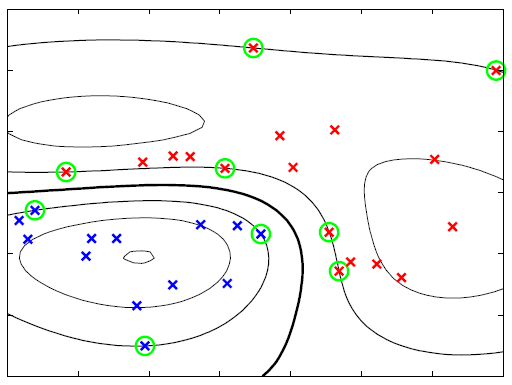
\includegraphics[width=\linewidth]{figures/SVMProd.png}\label{FigSVMProd}}
\end{figure}

\section{Disadvantages of Support Vector Machines}\label{PcSecIdea}
At first the \acs{SVM}, which is described as baseline classifier in section \ref{PcSecSVM}, provides a optimal solution through the convex optimization problem \cite[p. 325]{Bishop.2009}, but suffers from a few disadvantages.\newline
The \acs{SVM} is non probabilistic.
The problem is that the hard binary decisions which are made of the \acs{SVM} are not made to catch the uncertainty for predictions.
Furthermore, the probabilistic predictions are considered as crucial when posterior probabilities of a class assignment are adapted to varying class priors and asymmetric misclassification costs.\cite[p. 239-240]{Tipping.2001}\\
To solve this problem, there are some post processing methods developed to match the binary import to a probabilistic output.
However, this is considered as unreliable by \cite[p. 239-240]{Tipping.2001}. 
This uncertainty can be interpreted as Bayesian probability.\cite[p. 21]{Bishop.2009}\newline 
Second, the number of support vectors needed to create the margin of the decision boundary grows linearly with the size of the training set.
With that, the computational complexity and model complexity grows and does not lead to sparse models or fast computing.
As a consequence, some post-processing is suggested to reduce the complexity of the model.\cite{Chen.2009}\\
An example would be to find a set of 'reduced' vectors with $N_\mathcal{Z}$ entries, which are approximate the original set of support vectors $N_S$.
Note that these reduced vectors are no training samples and are not necessarily lying on the margin.
The goal is then to find the smallest $N_\mathcal{Z}$ with $N_\mathcal{Z} \ll N_S$ for that the loss in the generalisation performance is acceptable.
However, this approach is computational very expensive.\cite{Burges.1997}\\
Therefore the wanted reduction of computational complexity is maybe not yet achieved.\newline
Furthermore, the \ac{SVM} has several parameters, that needs to be tuned by cross-validation.
For example the $C$ parameter, explained in section \ref{PcSecSVM}, or the parameters for the kernel function for example the width of the Gaussian kernel, section \ref{EmSubSecKernel}.
Cross-validation is done by a grid search in a certain range.
For example evaluate the performance of the \ac{SVM} for $C={1,2,5,10,...,100,200}$ and select the parameter according to the best performance.\cite{Chen.2009}\newline
Finally, when it comes to the interpretation of the results, the \ac{SVM} provides a good interpretation of how the margin and the decision boundary is created.
However, the points which are considered as support vectors and therefore selected in the model, are not representing the actual data very well, because they are the closest points from one class to the other class.\cite[p. 326]{Bishop.2009}\newline
Here a key feature from the \ac{RVM} takes place. It creates a sparser model, in comparison with the \ac{SVM}, and provides a probabilistic estimate of the classes, where the relevance vectors are representing the data.\cite[p. 335-356]{Bishop.2009}\newline
This effect can be seen in figure \ref{FigRVMProbEst}.
One the right, the circled points are the relevance vectors of the model and on the right the posterior probability for the classes as colour gradient respectively.
\begin{figure}
	\centering
	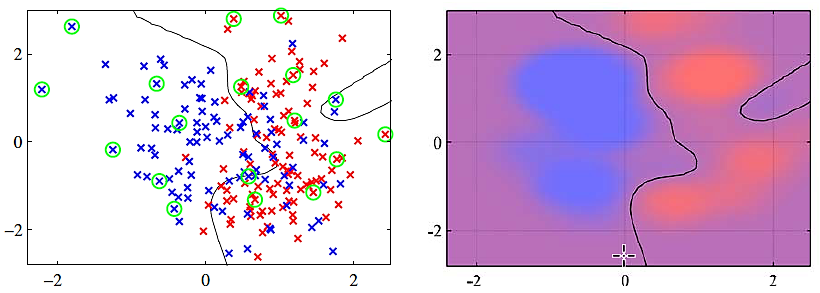
\includegraphics[width=.8\linewidth]{figures/RVMProbEst.png}
	\caption[Probabilitc Estimate of the RVM]{The probabilistic estimate of the \acs{RVM} on a synthetic dataset. The green circled points are relevance vectors.\cite[p. 356]{Bishop.2009}}
	\label{FigRVMProbEst}
\end{figure}

\section{Relevance Vector Machine}\label{PcSecRVM}
The \ac{RVM} is introduced by Tipping in the already noted work \cite{Tipping.2001}.
The key idea behind it is to create a classifier with a similar functional form to the \ac{SVM} with a probabilistic background. 
It uses a general Bayesian framework.\newline
The \acs{RVM} uses relevance vectors instead of support vectors.
It is found that for many weights the posterior distribution is sharply peaked around zero.
That means the probability for a certain weight for the training point is highest nearly the weight zero.
The training vectors with the corresponding remaining non-zero weights are called relevance vectors.
The weights representing the importance of a relevance vector.\cite[p. 213]{Tipping.2001}
Note that although in this thesis the same letter is used for the parameter $\mathbf{w}$, there is an important difference between them.
The \acs{SVM} defines with this parameter the hyperplane and the probabilistic vector machines are more prototypical vectors, which are representing the corresponding class in a probabilistic manner shown in figure \ref{FigRVMProbEst}.\cite[p. 222]{Tipping.2001}\newline
Another advantage of the \acs{RVM} against the \acs{SVM} is , that the kernel function for a \acs{SVM} has to satisfy Mercer's conditions.
The \ac{RVM} kernel does not have this constraint.\cite[p. 213]{Tipping.2001}\newline
Without going deeper in this, a kernel which satisfies the Mercer's conditions is positive semi-definite.\cite{Graepel.2002}
The complexity of the algorithm is $\mathcal{O}(M^3)$ with $M$ as number of basis functions and is also similar to the \ac{SVM}.\cite[p. 236-237]{Tipping.2001}\newline
The \ac{RVM} makes predictions for a new point $\mathbf{x}$ with equation \ref{EqRVMPred}.\cite[p. 211]{Tipping.2001}
\begin{equation}\label{EqRVMPred}
	\mathbf{t} = y(\mathbf{x};\mathbf{w}) = \sum_{i=1}^{N}\phi_i(\mathbf{x})w_i + w_0 = \boldsymbol{\Phi}(\mathbf{x})\mathbf{w} + w_0
\end{equation}
With the bias $w_0$ and basis function $\boldsymbol{\Phi}(\mathbf{x}) = (\phi(\mathbf{x_1}),\dots,\phi(\mathbf{x_n}))$.
The weight parameter has the form $\mathbf{w} = (w_1,\dots,w_N)^T$ and $\mathbf{T}={t_1,\dots,t_N}$ as function value.\\
In \eqref{EqRVMPred}, the bias is used to move the model out of the origin.
The corresponding label of a data point is the sign of the function value $\mathbf{t}$.
In general $t$ is the regression value. \cite[p. 662]{Theodoridis.2015} \newline
As a consequence, to being able to solve \eqref{EqRVMPred}, the weight $\mathbf{w}$ with size $N$ and $w_0$ has to be determined.
For the classification, the \acs{RVM} uses the Bayesian theorem in \eqref{EqBayesInfeRVM} do determine the weights $\mathbf{w}$. 
\begin{equation}\label{EqBayesInfeRVM}
	p( \mathbf{w}\vert \mathbf{t} ) \propto P(\mathbf{t}\vert \mathbf{w}) p(\mathbf{w} \vert \boldsymbol{\alpha})
\end{equation}
Note that the regression is varying from the classification solution.
The \ac{RVM} for classification gives the probability of a label for a point $\mathbf{x}$ by applying a logistic sigmoid function, with $y=y(\mathbf{x})$, which gives the probabilistic output:
\begin{equation}\label{EqLogSig}
	\sigma=1/(1+e^{-y}) 
\end{equation}
Furthermore, the logistic sigmoid function is combined with the Bernoulli distribution of $P(t\vert \mathbf{x})$ for the likelihood:
\begin{equation}\label{EqRVMLikelihood}
	P(\mathbf{t}\vert\mathbf{w})=\prod_{n=1}^{N}\sigma\{y(\mathbf{x}_n;\mathbf{w})\}^{t_n}[1-\sigma\{y(\mathbf{x}_n;\mathbf{w})\}]^{1-t_n}
\end{equation}
The Bernoulli distribution can be obtained from \cite[p. 685]{Bishop.2009} .
Additionally, the prior $p(\mathbf{w} \vert \boldsymbol{\alpha})$ is obtained by a zero-mean Gaussian:
\begin{equation}\label{EqRVMPrior}
	p(\mathbf{w} \vert \boldsymbol{\alpha}) = \prod_{i=0}^{N}\mathcal{N}(w_i\vert 0,a_i^{-1})
\end{equation}
With the inverse hyperparameter vector $\boldsymbol{\alpha}$ of size $N+1$ as the precision of the Gaussian.
At this point the parameter $w_0$ from \eqref{EqRVMPred} is determined.
The parameter $\boldsymbol{\alpha}$ itself is Gamma distributed.\cite[p. 214-215, 218-219]{Tipping.2001}\newline
An idea of a Gamma distribution and the Bernoulli distribution can be obtained from \cite[p.686-688]{Bishop.2009}.\newline
Because the integral of the Bayesian inference is intractable the following procedure is used to determine the parameters:
The algorithm is trained with the resulting Hessian Matrix from likelihood and prior of \ref{EqBayesInfeRVM}.
The most probable weights $\mathbf{w}_{MP}$ and the corresponding covariance matrix $\boldsymbol{\Sigma}$ are obtained from the mode of the posterior and the Hessian:
\begin{equation}
	\begin{split}
		\boldsymbol{\Sigma} = (\boldsymbol{\Phi}^T\mathbf{B}\boldsymbol{\Phi} + \mathbf{A})^{-1}\\
		w_{MP}=\boldsymbol{\Sigma}\Phi^T\mathbf{B}\mathbf{t} 
	\end{split}
\end{equation}
Where $\mathbf{A} = diag(\alpha_1,\dots,\alpha_N)$ and $\mathbf{B} = diag(\beta_1,\dots,\beta_N)$ with $\beta_n =\sigma\{y(\mathbf{x}_n)\}[1-\sigma\{y(\mathbf{x}_n)\}]$.
After the update of $\mathbf{w}_{MP}$ and $\boldsymbol{\Sigma}$ the hyperparameters are updated.
This is repeated until $\boldsymbol{\alpha}$ satisfies a stable convergence criteria.\cite[p. 219]{Tipping.2001}\newline
Although Tipping solved the problems of the \ac{SVM} with the \ac{RVM}, Chen et al. proposed that there are some concept problems left.\cite{Chen.2009}
These are discussed in the following sections, especially section \ref{PcSecWeights}.
\section{Probabilistic Classification Vector Machine}\label{PcSecAdvan}
In general, the \acf{PCVM} should provide a more stable solution, sparser model and better performance in comparison with the \acs{SVM} and \acs{RVM}.\cite{Chen.2009}\\
The \ac{PCVM} uses a latent variable model because of the assumption that the data is incomplete or latent.
Because of this and because the integral of the Bayesian Inference is in this case intractable, it uses an \ac{EM} algorithm, as it is a general solution to get a \ac{MAP} estimation of parameters based on latent variables.
Furthermore, the \acs{EM} algorithm optimises the parameters within, and therefore the \ac{PCVM} does not need cross-validation because the free model parameter is optimised within the algorithm.\cite{Chen.2009}\newline
An Attribute of the \acs{EM} algorithm is that it is likely to be trapped in local maxima and therefore finds no global solution.\cite{YiWang.2006}
Unlike to the \acs{SVM} which always can determine the global maxima, see section \ref{PcSecSVM}.\newline

\subsection{Model Specification}\label{PcSecCM}
The \acs{PCVM} is made for binary classification\cite{Chen.2009}, unlike the \acs{RVM}, which has a specification for multi class.\cite[p. 220]{Tipping.2001} But the ideas behind the two concepts are similar as we will see in the following.\\
In general, it makes predictions for a given test point $\mathbf{x}$ with the already known prediction function from \eqref{EqRVMPred} and \eqref{EqSVMPred}.\cite{Chen.2009}
As well as the \acs{RVM} in section \ref{PcSecRVM}, the \acs{PCVM} uses a link function to match the linear to a probabilistic output.
In the PCVM it is done with the probit link function defined in \ref{EqPcvmProbit}:\cite{Chen.2014}
\begin{equation}\label{EqPcvmProbit}
	\Psi(\mathbf{x}) = \int_{-\infty}^{x}N(t\vert 0,1)dt
\end{equation}
Where $\Psi$ is the Gaussian \ac{CDF}, with mean zero and variance one.\\
With a \ac{CDF} the probability for a new point x of a steady random variable X can be determined.
It is the integral of the density function and gives the probability $P(X \le x)$, which means the probability that X takes a value equals or less of x.\cite[p. 270]{Teschl.2014}\\
Therefore the probabilistic model after integrating the probit link function becomes:
\begin{equation}
	l(\mathbf{x};\mathbf{w};b) = \Psi\bigg(\sum_{i=1}^{N}w_i\phi_{i,\theta}(\mathbf{x}+b \bigg) = \Psi(\boldsymbol{\Phi}_\theta(\mathbf{x})\mathbf{w}+b)
\end{equation}
Where $\boldsymbol{\Phi(\mathbf{x})}_\theta=(\Phi_{1,\theta}(\mathbf{x}),\dots,\Phi_{N,\theta}(\mathbf{x}))$ and $\mathbf{w} = (w_1,\dots,w_N)^T$is the basis function vector with $N$ training data points.
$\theta$ is the parameter of the basis function. As the \ac{PCVM} uses the Gaussian kernel as basis function therefore the parameter $\theta$ is referred as the width of the kernel.\cite{Chen.2009}
The Gaussian kernel is described in the section \ref{EmSubSecKernel}.
\subsection{Prior over Weights}\label{PcSecWeights}
The three algorithms \acs{SVM}, \acs{RVM} and \acs{PCVM} are determining the weight parameter differently.\\
It is important for a stable solution that the sign of the weight $w_i$ of a data point $\mathbf{x}_i$ is equal to the corresponding classes $y_i \in\{-1,+1\}$.\cite{Chen.2009}\\
The \ac{SVM} ensures this by defining the weight vectors as $\mathbf{w} = \{v_1y_1,\dots,v_ny_n\}$, where $v_i$ are non negative Lagrange multipliers.
Therefore the same sign is guaranteed.\cite{Chen.2009}
But consider, that some of the data points which are not support vectors have $v_i=0$.\cite[p. 330]{Bishop.2009} \\
The \ac{RVM} estimates the weights according to equation \eqref{EqBayesInfeRVM}.
The likelihood is always positive because exponential function $e$ is always positive \cite[p. 355]{Hartmann.2015} and hence the logistic sigmoid link function is it.
Therefore the sign depends on the prior, which uses the zero-mean Gaussian over all weights and hence providing some problems.\\
It can happen that training errors occur with the use of the zero-mean Gaussian because the weight of a positive relevance vector can get a negative weight assigned and vice versa.
This may lead to an unstable result corresponding to nonreliable vectors.
As a consequence, the \acs{RVM} is more likely to overfit the noise in comparison with the \acs{SVM} and \acs{PCVM}, with the same selection of parameters.\cite{Chen.2009}\\
At this point the improvements of the \acs{PCVM} take place. 
Instead of the zero-mean Gaussian prior, it uses the zero-mean truncated Gaussian as prior. \cite{Chen.2009}
\begin{equation}\label{EqPcvmNtPrior}
	p(\mathbf{w} \vert \boldsymbol{\alpha}) = \sum_{i=1}^{N}p(w_i \vert \alpha_i) = \sum_{i=1}^{N}N_t(w_i \vert 0,\alpha_i^{-1})
\end{equation}
Here $N_t$ is the truncated Gaussian function with $\alpha$ as inverse variance.\\
With that, the relevance vector is always getting the proper signed weight attached.
Because for $y_i=+1$ the prior is selected from the right-truncated non-negative Gaussian and for $y_i=-1$ it is the left-truncated non-positive Gaussian.\cite{Chen.2009}\\
Now to avoid errors corresponding to noise or unreliable points the above is formulated in \eqref{EqPcvmWSel}.\cite{Chen.2009}
\begin{equation}\label{EqPcvmWSel}
	p(w_i \vert \alpha_i) =
	\begin{dcases*}
		2N(w_i \vert 0,\alpha_i^{-1} ),\>\>\>\>  if y_i w_i \ge 0\\
		0				,\>\>\>\>\>\>\>\>\>\>\>\>\>\>\>\>\>\>\>\>\>\>\>\>\>\>\>\> if y_i w_i<0
	\end{dcases*}
\end{equation}
With that, the \acs{PCVM} assigns for an unreliable point a zero weight, and therefore there it is no longer considers as relevance vector for the model.
The truncated Gaussian priors are illustrated in figure \ref{FigTruncGaus}.\newline
The bias $b$ which is referred as $w_0$ in \eqref{EqRVMPrior} is still determined with the zero-mean Gaussian:\cite{Chen.2009}
\begin{equation}\label{EqPcvmBPrior}
p(b \vert \beta) = N(b \vert 0, \beta^{-1})
\end{equation}
\begin{figure}
	\centering
	\floatbox[{\capbeside\thisfloatsetup{capbesideposition={right,top},capbesidewidth=6cm}}]{figure}[\FBwidth]
	{\caption[Truncated Gaussian Priors over Weights]{The truncated Gaussian priors over weights.On the left side the non positive left-truncated one in case of a negative class labels. On the right side the non negative right-runcated one for the positive class.\cite{Chen.2009}}}
	{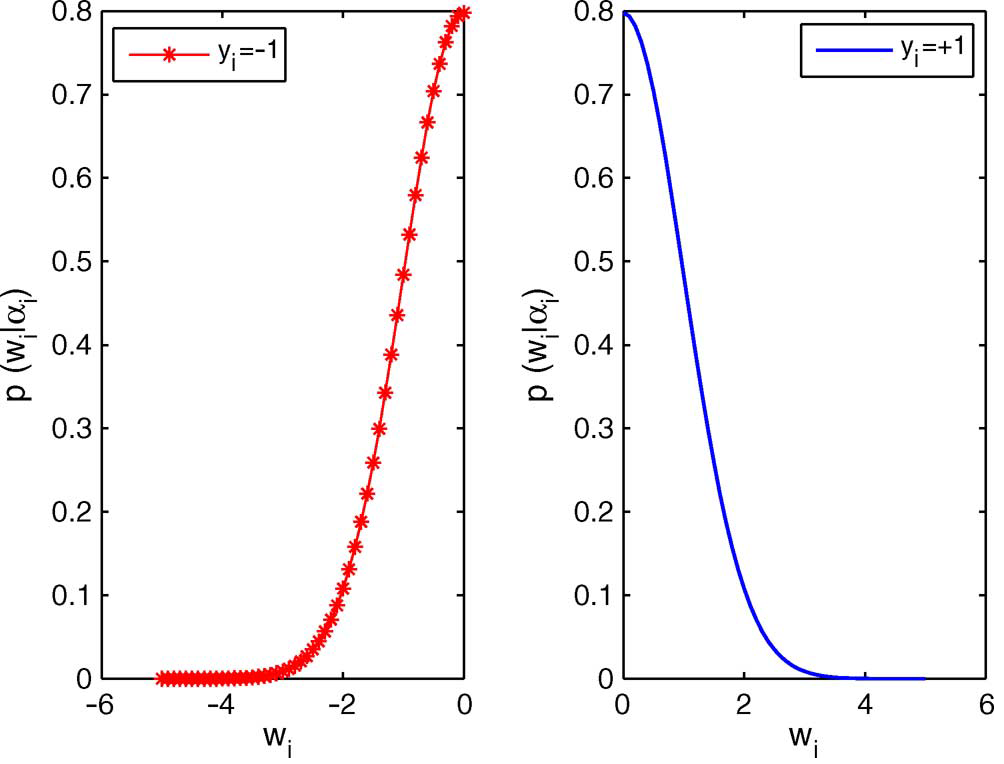
\includegraphics[width=\linewidth]{figures/TuncatedGaussian.png}\label{FigTruncGaus}}
\end{figure}
\subsection{Expectation Maximization Algorithm}\label{PcSecEM}
The \acs{PCVM} uses a simple latent variable model within the \acs{EM} algorithm.\cite{Chen.2009}
A latent variable can either be missing data or is unobservable.\cite[p. 276-277]{TrevorHastie.2009}
The latter is sometimes called hidden and can be for example class labels or parameters and has to be determined.\cite[p. 84]{Bishop.2009}
Hidden in this context means this variable can not be directly observed and his existence is implicit.\cite{Borsboom.}\\
The difference between a parameter and a latent variable in this thesis is that the parameter should be learned through the learning algorithm based on the data.
The latent variable is a part of the data which is not available (hidden) but is involved in the model.
Therefore the algorithm takes assumptions to deal with the uncertainty of this latent variables.\\
The standard probabilistic assumption is that the formulation in \eqref{EqRVMPred} is affected.
Therefore \eqref{EqRVMPred} can be reformulated as \eqref{EqPcvmRessNoise}.\cite{Chen.2009}
\begin{equation}\label{EqPcvmRessNoise}
	h_\theta (\mathbf{x}) = \boldsymbol{\Phi}_\theta(\mathbf{x}) \mathbf{w} + b +  \epsilon
\end{equation} 
With the $\theta$ parameter for the basis function and the bias $b$ instead of $w_0$.
The noise is distributed according to the standard Gaussian as $\epsilon \sim N(0,1)$.
Furthermore, because $\epsilon$ is unobservable thus latent, the $h_\theta(\mathbf{x})$ itself will be considered as latent variable.\cite{Chen.2009}\\
The \acs{PCVM} uses the probit link function, which is used for regression.\cite{Albert.1993}. It gives a variable $l = 1$, when the corresponding $h_\theta (\mathbf{x}) \ge 0$ and $l = 0$ for $h_\theta (\mathbf{x}) < 0$.\cite{Chen.2009}.
Therefore, to obtain the probit mode, the Gaussian \acs{CDF} is used.
\begin{equation}\label{EqProbitLinkProb}
	P(l=1\vert x,w,b) = p(\boldsymbol{\Phi}_\theta(\mathbf{x})\mathbf{w} + b + \epsilon \ge 0) = \Psi(\boldsymbol{\Phi}_\theta(\mathbf{x})\mathbf{w} +b)
\end{equation}
It states, given the data $\mathbf{x}$ and the parameter $\mathbf{w}$ and $b$, how likely is it that it belongs to the positive class.
To get the probability for the other class it is simply $P(l=0 \vert x,w,b) = 1-P(l=1\vert x,w,b)$.\cite{Chen.2009}\\
Revisiting \eqref{EqRVMPred}, we need to determine $\mathbf{w}$ for the model.
Again the Bayesian theorem is used to determine most probably parameter values.\cite{Chen.2009}\\
The prior for $\mathbf{w}$ is already obtain through \ref{EqPcvmNtPrior} and the bias is specified with \eqref{EqPcvmBPrior} as zero-mean Gaussian. Therefore only the likelihood has to be specified.
Taking the assumption that $h_\theta (\mathbf{x})$ is known, the Gaussian likelihood could be obtained with:\cite{Chen.2009}
\begin{equation}\label{EqPcGausLike}
\begin{gathered}
	p(\mathbf{H}_\theta(\mathbf{x})\vert w,b) = N(\mathbf{H}_\theta(\mathbf{x})\vert \mathbf{\Phi}_\theta(x)\mathbf{w}+b,1)\\
	= (2\pi)^{N/2}\exp\{-\frac{1}{2} \abs{\mathbf{H}_{\theta} - \mathbf{\Phi}_{\theta}\mathbf{w}+b\mathbf{I}}^2 \}
\end{gathered}
\end{equation}
With $\mathbf{H}_\theta(\mathbf{x}) = (h_\theta(\mathbf{x}_1),\dots,h_\theta(\mathbf{x}_N))^T$ and where $\mathbf{\Phi_\theta} = (\mathbf{\Phi}_\theta(\mathbf{x}_1)^T,\dots,\Phi_\theta(\mathbf{x}_N)^T)^T$ and $\mathbf{\Phi}_\theta(\mathbf{x_i}) = (\phi(\mathbf{x}_1,\mathbf{x}_i),\dots,(\phi(\mathbf{x}_N,\mathbf{x}_i))$ forming the kernel.
At this point it is important reintroduce a clear notation.
$\mathbf{\Phi}_\theta$ as kernel. Within this kernel $\mathbf{\Phi}(\mathbf{x}_i)$ is a row and $\mathbf{\Phi}_\theta(\mathbf{x})$ refers to the row corresponding to $\mathbf{x}$.\\
For the complete log-posterior of the parameters $\mathbf{w}$ and $b$ the corresponding parameters, $\alpha$ and $\beta$ are also considered as latent variables.
With that, there are three latent variables in the posterior.
Instead of the standard posterior, the $\log$ posterior is used and therefore has the form:\cite{Chen.2009}
\begin{equation}\label{EqPcvmInf}
\begin{gathered}
	\log p(\mathbf{w},b\vert \mathbf{y},\mathbf{H}_\theta,\alpha,\beta) \propto \log p(\mathbf{H}_\theta \vert \mathbf{w},b) + \log p(\mathbf{w}\vert \alpha) + \log p(b\vert \beta)\\
	\propto \mathbf{w}^T\mathbf{\Phi}_\theta^T(2\mathbf{H}_\theta - \mathbf{\Phi}\mathbf{w})+2b\mathbf{I}^T\mathbf{H}_\theta - 2b\mathbf{I}^T\mathbf{\Phi}_\theta - b^2N - \mathbf{w}^T\mathbf{Aw}-\beta b^2
\end{gathered}
\end{equation}
With that, we can proceed with the \acs{EM} algorithm.\cite{Chen.2009}\\
The \acs{EM} algorithm was originally introduced by Dempster et al. and is made for determining the maximum likelihood for incomplete data \cite{Dempster.1977}. 
Based on their work, many other applications are made to determine parameters.
For example Bishop used a \acs{EM} algorithm within the algorithm $k$-means cluster.\cite[p. 426-428]{Bishop.2009}
Furthermore, Hasti et al. using it in \cite[p. 272-276]{TrevorHastie.2009} for a two-component mixture model.\
Although Tipping never mentioned the use of the \acs{EM} algorithm in the \acs{RVM}, the procedure of it, explained in \ref{PcSecRVM} is similar.\cite[p. 233-234]{Tipping.2001}.
Furthermore, he introduced an Expectation-Maximisation Update approach for determining the parameters.\cite[. 235]{Tipping.2001} \newline
As the name says, it consists of two steps.
The algorithm has the $E$ and $M$ steps per iteration, and will repeat as long as a convergence criterion is reached or the maximum iteration is reached, which can be specified in algorithm \ref{PcSubSecAlgo}.
The first, the Expectation-Step finds expectations for the latent variables and furthermore an expectation for posterior of the parameters, which is referred as $\mathcal{Q}$ function.
In the case of the \acs{PCVM} it has the form:\cite{Chen.2009}
\begin{equation}\label{EqPcvmEStep}
\begin{gathered}
	\mathcal{Q}(\mathbf{w},b\vert \mathbf{w}^{old},b^{old}) = E_{\mathbf{H}_{\theta},\alpha,\beta}[\log p (\mathbf{w},b \vert \mathbf{y} ,\mathbf{H}_{\theta},\alpha,\beta) | y,\mathbf{w}^{old},b^{old}]\\
	= 2\mathbf{w}^T \mathbf{\Phi}_{\theta}^T \expB{\mathbf{H}}_\theta - \mathbf{w}^T \mathbf{\Phi}_{\theta}^T  \mathbf{\Phi}_{\theta} \mathbf{w} + 2b\mathbf{I}^T \expB{\mathbf{H}}_{\theta} -  b^2N + 2b\mathbf{I}^T \mathbf{\Phi}_\theta \mathbf{w}- \mathbf{w}^T\expB{\mathbf{A}}\mathbf{w} - \expB{\beta}b^2
\end{gathered}
\end{equation}
With $\mathbf{\expB{H}}_\theta =  E[\mathbf{H}_\theta \vert y, \mathbf{w}^{old}, b^{old}]$, $\mathbf{\expB{A}} = diag(E[\alpha_i|y_i,\mathbf{w}^{old},b^{old}])$ and $\expB{\beta}=E[\beta\vert y_i,\mathbf{w}^{old},b^{old}]$.
For details to the determination the expectation, see Appendix B in \cite{Chen.2009}.\\
This step relies on the 'old' latent variables and parameters from the previous iteration.
The next part in the iteration is the Maximization-Step.\cite{Chen.2009}\\
Revisiting \ref{EqPcvmEStep}, $\mathcal{Q}$ gives the expectation of the posterior distribution based on the current state of all variables and parameters. 
Therefore by analysing \ref{EqPcvmEStep}, the algorithm gives the most probable expectations for the posterior for the parameters with respect to the latent variables and the old parameters. \\
In this algorithm, the maximum is found by analysing the derivatives of the $\mathcal{Q}$ function with respect to $\mathbf{w}$, $b$ and $\theta$.
The latter is optimized because the Algorithm is designed to optimize his selectable parameter to avoid cross validation.\cite{Chen.2009}\\
A joint maximization of $\mathcal{Q}$ can not be done and therefore the parameters are optimized one after the other by set the derivatives to $\frac{\partial \mathcal{Q}}{\partial \mathbf{w}} = 0$ and $\frac{\partial \mathcal{Q}}{\partial b} = 0$ and solving the equation for $\mathbf{w}$ and $b$ respectively the update rules are obtained:\cite{Chen.2009}
\begin{equation}\label{EqPcvmUpdateW}
	\mathbf{w}_{new} = (\mathbf{\Phi}_\theta^T \mathbf{\Phi}_\theta + \mathbf{\expB{A}})^{-1} (\mathbf{\Phi}_\theta^T \expB{\mathbf{H}}_\theta - b\mathbf{\Phi}_\theta^T \mathbf{I})
\end{equation}
\begin{equation}\label{EqPcvmUpdateb}
	b^{new} = \frac{\mathbf{I}^T \expB{\mathbf{H}}_\theta - \mathbf{I}^T \mathbf{\Phi}_\theta \mathbf{w}}{\beta + N}
\end{equation}
With that the maximum is found and therefore the 'new' parameters for $\mathbf{w}^{old}$ and $b^{old}$ for \ref{EqPcvmEStep} are found for the next iteration.
The optimization for $\theta$ is done by a conjugate gradient algorithm\footnote{http://learning.eng.cam.ac.uk/carl/code/minimize/} which is done on basis of \eqref{EqPcvmDevTheta}.\cite{Chen.2009}
\begin{equation}\label{EqPcvmDevTheta}
	\frac{\partial \mathcal{Q}}{\partial \mathbf{\theta}_k } = 2 \sum_{i=1}^{N}\sum_{j=1}^{N} \bigg\{ (\mathbf{\Phi}_\theta \mathbf{w} - \expB{\mathbf{H}}_\theta) \mathbf{w}^T \odot (\frac{\partial\mathbf{\Phi}_\theta}{\partial \theta_k} ) \bigg\}_{(i,j)}
\end{equation}
With $\odot$ as Hadamard matrix multiplication as defined in \cite{CaroLopera.2012}.\newline
\subsection{Algorithm}\label{PcSubSecAlgo}
In the following the pseudo code of \acs{PCVM} is presented in algorithm \ref{PseudoCodePcvm}.
\begin{algorithm}[H]
	\caption{Probabilistic Classification Vector Machine}\label{PseudoCodePcvm}	
	\begin{algorithmic}[1]
		\Require $\mathbf{I}$ =\{\textbf{X,Y}\} = $\{(x_n,y_n)\}_{n=1}^{N}$ as $N$-sized training set;
		\textit{ker} as kernel type; The kernel parameter $\theta$; \textit{niter} as maximal number of iterations; \textit{threshold} as convergence criteria; \textbf{InitVector} as $N$-sized initialization vector.
		\Ensure Weight Vector $\mathbf{w}$, bias $b$ and the kernel parameter $\theta$.
		\State	[$\mathbf{w},b$] = initialize(\textbf{initVector});
		\State \textbf{nonZero} = determine\_nonZero\_Vector($\mathbf{w}$); 
		\For{$i=1$ to \textit{niter}}
			\State $\Phi$ = Calculate\_Kernel($\mathbf{X,Y}$,\textit{ker},$\theta$); 
			\State $\mathbf{w}^{new}$ = weight\_update($\mathbf{\Phi,w,Y,nonZero}$);  
			\State $b^{new}$ = bias\_update = bias\_update($\mathbf{\Phi},b,\mathbf{Y,nonZero}$);
			\State $\theta^{new}$ = parameter\_update($\mathbf{\Phi,X,Y},\mathit{ker},\theta,\mathbf{w}^{new},b^{new},\mathbf{nonZero}$);
			\State $\mathbf{nonZero}^{new}$ = determine\_nonZero\_Vector($\mathbf{w}^{new}$);
				\If{max(abs($\mathbf{w}^{new}-\mathbf{w}$)) $<$ \textit{threshold}}
					\State break;
				\Else
					\State continue;
				\EndIf
		\EndFor
	\end{algorithmic}
\end{algorithm}
\algcomment{Explanation of the Steps within the Algorithm.
	\begin{enumerate}[noitemsep]
		\item Line 1 and 2: (Random) initialization of the weight vector $\mathbf{w}$ with $N$-sized \textbf{initVector} and bias $b$. Determining non zero elements in $\mathbf{w}$ and save it as index to \textbf{nonZero}.
		\item Line 4: Calculate the kernel $\Phi$.
		\item Line 5 and 6: Update $\mathbf{w}$ and $b$ with \eqref{EqPcvmUpdateW} and \eqref{EqPcvmUpdateb} respectively.
		\item Line 7: Solve optimization problem based on \eqref{EqPcvmDevTheta}.
		\item Line 9-15: Determine the convergence by comparing the difference of $\mathbf{w}^{new}$ and $\mathbf{w}$ against the threshold. Break if convergence happens, otherwise continue.
	\end{enumerate}}\\
It can be seen in algorithm \ref{PseudoCodePcvm} that the convergence of the algorithm is only measured with the convergence behaviour of $\mathbf{w}$ and is set to $||{\mathbf{w}-\mathbf{w}^{old}}|| = 1.0e^{-3}$ in practice. 
The time complexity of the \acs{PCVM} is $\mathcal{O}(N^3)$, with N as the number of training points.\\
In practice the Cholesky decomposition is used for the matrix inversion. 
This has the computational complexity of $\mathcal{O}(M)^3$ and a memory complexity of $\mathcal{O}(M)^2$, where M is the number of non zero basis functions and is the overall complexity of the \acs{PCVM}.\cite{Chen.2009}\\
However, because of the sparsity of the prior, the \acs{PCVM} reduces the basis function from the initial start with $M = N$ to $M < N$.
In the best case it be even $M \ll N$.
An practical example of this reduction can be found in table \ref{BTableFTNev} in appendix \ref{appaB}. 
This table shows the number of vectors which are needed for the model. 
It can be seen that the \acs{PCVM} has a sparser model in comparison to the \acs{SVM} and has therefore less basis function.

\subsection{Hierachical Hyperpriors}\label{PcSubSecHierHyper}
In the section \ref{PcSecWeights} the priors are introduced with the $N$ sized parameter vector $\boldsymbol{\alpha }$ and $\beta$.
Although they are already defined, they can alternatively be controlled with hierarchical hyperparameters regarding the Bayesian Framework.
This means that hyperparameters are controlling the distribution of the prior. \cite[p. 71]{Bishop.2009}
Because these hyperparameters are controlled by a prior of another distribution, this prior is called hyperprior.\cite[.p 423]{Bishop.1995}\\
The \acs{PCVM} uses the gamma distribution for modelling the hyperprior:\cite{Chen.2009}
\begin{equation}\label{EqPcvmHyperParameter}
\begin{gathered}
		p(\boldsymbol{\alpha}) = \prod_{i=1}^{N}Gamma(\alpha_i \vert c,d)\\
		p(\beta) = Gamma(\beta\vert e,f)
\end{gathered}
\end{equation}	
With using the hyperparameters $c,d,e$ and $f$ the prior can be obtained by marginalizing out $\alpha_i$ in \ref{EqWPriorMa} and $\beta$ in \ref{EqBPriorMb}:\cite{Chen.2009}
\begin{equation}\label{EqWPriorMa}
	\begin{gathered}
		p(w_i \vert c,d) = \int_{0}^{\infty} p(w_i \vert \alpha_i)p(\alpha_i\vert ,c,d)d\alpha_i \\ 
		=\begin{dcases}
				\frac{2d^c\Gamma(c+\frac{1}{2})}{\sqrt{2\pi}\Gamma(c)}\bigg(\frac{w_i^2}{2}+d \bigg)^{-(c+\frac{1}{2})}, if y_iw_i \ge 0\\ 
				0, \>\>\>\>\>\>\>\>\>\>\>\>\>\>\>\>\>\>\>\>\>\>\>\>\>\>\>\>\>\>\>\>\>\>\>\>\>\>\>\>\>\>\>\>\>\>\>\>\>\>\>\> if y_i w_i<0
		\end{dcases}
	\end{gathered}
\end{equation}
\begin{equation}\label{EqBPriorMb}
	\begin{gathered}
		p(b\vert e,f) = \int_{0}^{\infty} p(b \vert \beta) p(\beta \vert e,f)d\beta \\
		=\frac{f^e\Gamma(e + \frac{1}{2})}{\sqrt{2\pi}\Gamma(e)}\bigg( \frac{b^2}{2}+f\bigg)^{-e+\frac{1}{2})}
	\end{gathered}
\end{equation}
Which form the hierarchical hyperprior.\cite{Chen.2014} These are equivalent to the truncated student-t prior over $\mathbf{w}$ and the student-t prior over b.\cite[p. 226]{Tipping.2001}\newline
This student-t prior is more sharply and peaked about zero than the Gaussian prior\cite{Chen.2009}, which can be seen in \cite[p. 688, 691-692]{Bishop.2009}.\newline
In practice the hyperparameters $c,d,e$ and $f$ are set to zero and therefore the prior of $\mathbf{w}$ can be formalized as in \ref{EqWPriorMwZero}.
\begin{equation}\label{EqWPriorMwZero}
	p(w_i) =
	=\begin{dcases}
	\frac{2\Gamma(\frac{1}{2})}{\sqrt{2\pi}\Gamma(0)}\bigg(\frac{w_i^2}{2} \bigg)^{-\frac{1}{2}}, if y_iw_i \ge 0\\ 
	0, \>\>\>\>\>\>\>\>\>\>\>\>\>\>\>\>\>\>\>\>\>\>\>\>\>\>\>\>\>\>\>\>\> if y_i w_i<0
	\end{dcases}
\end{equation}
The hierarchical hyperprior for $b$ can be obtained analogue to equation \eqref{EqWPriorMwZero}. This prior can be interpreted as Laplacian prior and leads to sparsity.\cite{Chen.2009} 
An idea of the multivariate Laplacian distribution can be obtained from \cite{Eltoft.2006}.
\subsection{Implementation Details}\label{PcSubSecImplementation}
In the last section of this chapter, some changes in the formulations are introduced to make the algorithm more stable in practice.
The Expectation of the latent variables for $\expB{\alpha_i}$ and $\expB{\beta}$ are calculated with:\cite{Chen.2009}
\begin{equation}\label{EqPcvmLatenHyp}
		\expB{\alpha}_i = \frac{c + \frac{1}{2}}{w_i^2 + d} \>\>\>\>\>\>\>\>\>\>\>\>\>\>\>
		\expB{\beta} = \frac{c + \frac{1}{2}}{b^2 + f}
\end{equation}
See Appendix B of \cite{Chen.2009} for details of the expectation derivation of $\expB{\alpha}_i$ and $\expB{\beta}$.\\
With that according to \ref{PcSubSecHierHyper} the hyperparameters are set to zero.
Because of the fact that $\alpha_i$ are inverse proportional to the square  $w_i$, the parameter vector can be rewritten as $\expB{A} = diag[(\sqrt{2}w_1)^{-2},\dots,(\sqrt{2}w_N)^{-2}]$.
As consequence the expectation changes to $\expB{\alpha_i} = (1/2w_i)$ and because of the sparse model many values of $w_i$ tends towards zero and therefore it may become unstable.\cite{Chen.2009}\\
Revisiting the weight may become very small and leads to large numbers in $\expB{\mathbf{A}}$. Therefore the matrix $\mathbf{M}=diag[\sqrt{2}w_1,\dots,\sqrt{2}w_N]$ with $(\mathbf{M}^{-1})^{-2}$ is used, which is suggested in \cite{Figueiredo.2003}.
This avoids the inversion of the elements $w_i$ at the update state (M-Step). This modification is applied to $b$ and $\mathbf{w}$ and therefore the equations from \ref{EqPcvmUpdateW} and \ref{EqPcvmUpdateb} changes to:\cite{Chen.2009}
\begin{equation}\label{EqPcvmStableUpdate}
	\begin{gathered}
	\mathbf{w}^{new} = \mathbf{M}(\mathbf{M \Phi}_\theta^T\mathbf{\Phi}_\theta\mathbf{M}+\mathbf{I}_n)^{-1} \mathbf{M}(\mathbf{\Phi}_\theta^T\expB{\mathbf{H}}_\theta - b \mathbf{\Phi}_\theta^T \mathbf{I}_N)\\
	b^{new} = t(1 + tNt)^{-1} t(\mathbf{I}^T\expB{H}_\theta-\mathbf{I}^T\mathbf{\Phi}_\theta\mathbf{w})
	\end{gathered}
\end{equation}
With the $N\times N$ identity matrix $\mathbf{I}$ and $t=\sqrt{2}|b|$.
Furthermore, the diagonal matrix elements of M are:
\begin{equation}\label{EqPcvmMDiag}
	m_i = \expB{\alpha_i}^{-1/2} = 
	\begin{dcases}
		\sqrt{2}w_i,\>\>\> if y_iw_i \ge 0 \\
		0, \>\>\>\>\>\>\>\>\>\>\> if y_iw_i < 0		
		\end{dcases}
\end{equation}
This changes should allow a stable numerical calculation.\\
However, this changes may not avoid the fact that some diagonal elements of $\expB{\mathbf{A}}$ in $(\mathbf{\Phi}_\theta\mathbf{\Phi}+\expB{\mathbf{A}})$ becoming very large and therefore the matrix becomes numerical singular.
This happens when $w_i$ tends towards zero.
To avoid this, the kernel column of the corresponding very small weight is deleted. \cite{Chen.2014}\newline
As already mention for the matrix inversion the Cholesky decomposition is used.\cite{Chen.2014} The Cholesky decomposition is considered as numerical stable.\cite[p. 101]{Press.2007}\\
Note that because of the zero-mean Gaussian assumption, i\,e. $N(0,1)$ the datasets for training and testing for the \acs{PCVM} has to be z-scored.
Refer to equation \eqref{EqZTrans} in section \ref{InSubSecTheta} for this.
\section{Conclusion}
Summarizing, Chen et al. have proposed the \acs{PCVM} as improvement to the \acs{SVM} and \acs{RVM}.
They have evaluated this statement, in a performance study on three synthetic datasets and 12 benchmark datasets.
They determined statistical significance with the 5x2 cv F test and the Friedman test.
The result of this study is that the \acs{PCVM} can outperform the \acs{RVM} and \acs{SVM}.
In fact the \acs{PCVM} has the same advantages over \ac{SVM} as the \acs{RVM} has and furthermore uses a more reasonable prior.\cite{Chen.2009}

\chapter{Transfer Learning}\label{Tl}
In this chapter, the technique of transfer learning will be introduced.
It can be considered as a large interpretation of related work.\\
This Chapter is organized as follows:    
First of all, we discuss some challenges of the traditional machine learning algorithms.
Furthermore, some real world and machine learning sample problems are discussed.\\
In the second section, the task transfer learning in the context of classification will be described.\\
There are various definitions of transfer learning in general.
Many of the solutions obtained in this chapter are made for different definitions.
Moreover, because of this the difficulty of the problem which is solved by the solutions may vary, see \ref{TlSecDef}.\\
Additionally, we will see how the difference in transfer learning is measured.\\
Furthermore, the settings of transfer learning will be introduced.
The settings implying the different setups to solve the transfer problem.\\
In the next section will introduce and explain the two main types of the transfer learning which describes the conditions of the feature space and probability distributions.
These types can be divided into approach categories.
Most of the discussed solutions are based on the formal ideas of a category.\\
The section, negative transfer deals with the problem that the provided transfer learning solutions are in fact worse than the baseline methods.
For details to kernels see section \ref{EmSubSecKernel}.

\section{Challenges of Machine Learning Algorithms}\label{TlSecChal}
The current state of 'traditional' machine learning algorithms is the assumption that training and test data existing in the same feature space and that they have the same distribution.
They are successfully learning patterns and predict events in the future.
However, it is not always possible to obtain training and test data, which matches in distribution or features space.
Reason for this may that training data, which has to be labelled, is expensive or difficult to achieve.\cite[p. 1]{Weiss.2016}\\
When it comes to supervised learning, the algorithms are designed in a way to learn from the pre-labelled data and hence it is crucial for this types of algorithms to have some.\cite[p. 6-7]{Theodoridis.2008}\\
In the 'traditional' manner, which applies to the most statistical models, to solve the problem of differences, they have to collect new training data for the new feature space or distribution of the test data and rebuild the model.\cite{Pan.2010}
Therefore, the good performance cannot be obtained, when the training and test data differs in feature space or distribution.
This is the reason, one has to find a classifier, which can be applied to the target domain, although it is trained on the source domain, which is the main motivation of Transfer Learning.\cite[p. 1.]{Weiss.2016}\\
A simple interpretation of Transfer Learning in the real world is given in the following:
Imaging two people, who want to learn piano.
One has never played any musical instrument before, while the second has previous collected knowledge on how to play music through experience with other instruments.
The latter will be able to learn the new instrument much faster than the first with no previous experience because he can transfer his general music knowledge to boost his learning of the new instrument.\cite[p. 1]{Weiss.2016}\\
When going back to machine learning, there are be more technical examples.
Consider the task of web document classification.
The goal is to classify web documents in predefined categories.
The training data in this example are university web pages, which are associated with a category by manual labelling.
If we want to classify our test data, which may not come from a university page and as a consequence the data features or distribution may be different, based on the structure or topics of the new web page.
Therefore, we can not directly apply the classifier trained on the university web page and assume a good category prediction rate on non-university web pages.
Instead, we have to collect new websites from the same type as of the test web pages, assign the category manually and finally learn a new model.
This process could be avoided if a classifier can transfer knowledge from one domain of pages into another web page domain.\cite{Pan.2010}\\
The last example is given from the topic of product reviews.
Consider the problem that a model needs to be learned, in a way that it can automatically classify positive and negative reviews on a product.
To create a source domain, one has to collect many reviews of the product and manually decide if it is positive or negative.
Then the model can be trained and can predict the sentiment of new reviews.
However, if the product changes, then the distribution of the review may change, and the traditionally learned classifier cannot be applied anymore.
Therefore, again one has to collect reviews manually and annotate them.
This can be a very expensive process, and therefore the learner should be adaptable that it can be learned on the source domain (one product category) and can help to learn the classification model (other product category).\cite{Pan.2010}

\section{Definition of Transfer Learning}\label{TlSecDef}
After more practical examples are given, the term transfer learning and associated keywords are defined in this section.\newline
In this thesis, a domain $\mathcal{D}$ is composed of a $D$-dimensional feature space $\mathcal{F}$ and a marginal probability distribution $P(\mathbf{X})$.
Formally, this means $\mathcal{D} = \{\mathcal{F},P(\mathbf{X})\}$ with $\mathbf{X} \in \mathcal{F}$.
In general, if two domains $\mathcal{X}$ and $\mathcal{Z}$ are different, then they have either different feature spaces or marginal distributions.
This can be expressed as $\mathcal{F_{Z}} \neq \mathcal{F_{X}} \vee P(x) \neq \textit{P}(z)$.\cite[. 542]{Aggarwal.2015}\\
A task $\mathcal{T}$ with a given domain D is put together with a label set $\mathcal{Y}$ and a classifier $f(\cdot)$, which is  $\mathcal{T} = \{\mathcal{Y},\textit{f}(\cdot)\}$ with $\mathbf{y} \in \mathcal{Y}$.
The function $f(\cdot)$ is a predictive function to make prediction for unseen, i.\,g. new data points $\mathbf{x}$.
From a probabilistic viewpoint we can interpret $f(x)$ as $P(y\mid x)$.
In other words given x how probable is it that label y is correctly assigned.\\
In classification, the number of varying labels will distinguish the classification problem.
The Binary classification problem for two labels, e.\,g. $\mathcal{Y} ={-1,+1}$ or discrete values, i.\,e. multiple classes, for example $\mathcal{Y}= \{1,2,..,N\}$ with $N$ classes.
In general two tasks $\mathcal{T_X}$ and $\mathcal{T_{Z}}$ are different if they have varying conditional probability distributions or label spaces, which means $\mathcal{Y_{X}} \neq \mathcal{Y_{Z}} \vee P(y\mid x) \neq P(y\mid z)$.\cite[p. 542]{Aggarwal.2015}\\ 
Note that in this thesis if we talk about transfer learning, then the training domain is denoted as $\mathcal{Z}$ and $\mathcal{X}$ represents the test domain.
For the binary case within transfer learning the following definitions are made:
Consider $\mathbf{Z} = \{(\mathbf{z}_i,y_{\mathcal{Z}_i})\}_{i=1}^{M}$ as source domain data where $\mathbf{z}_i \in \mathcal{X}_\mathcal{Z}$ as single observation and $y_{\mathcal{Z}_i} \in \mathcal{Y}_\mathcal{Z}$ is the corresponding class label, which forms the whole label vector $\mathbf{y}_\mathcal{Z}$.
Additional, the target domain data $\mathbf{X} = \{(\mathbf{x}_i,y_{\mathcal{X}_i})\}_{i=1}^{N}$.
Analogue, $\mathbf{x}_i$ is a single observation with $\mathbf{x}_i \in \mathcal{X}_\mathcal{X}$ and the corresponding class label $y_{\mathcal{X}_i} \in \mathcal{Y}_\mathcal{X}$, which is again summarized in $\mathbf{y}_\mathcal{X}$.\cite[p. 2]{Aggarwal.2015}\\
Note that we are doing the assumption here that our problem has by default more than one dimension and therefore we write a single observation as a vector of features.
The whole data is therefore represented as a matrix.
\begin{mDef}[Transfer Learning]\label{DefTl}
	Given a source domain $\mathcal{Z}$ and learning task $\mathcal{T}_\mathcal{Z}$, a target domain $\mathcal{X}$ and learning task $\mathcal{T}_\mathcal{X}$, transfer learning aims to help improve the learning of the target predictive function $f_\mathcal{X}(\cdot)$ in $\mathcal{X}$ using the knowledge in $\mathcal{Z}$ and $\mathcal{T}_\mathcal{Z}$, where $\mathcal{Z} \neq \mathcal{X}$, or $\mathcal{T}_\mathcal{Z} \neq \mathcal{T}_\mathcal{X}$.\cite[p. 542]{Aggarwal.2015}
\end{mDef}
Summarizing, our problem consist of $\mathcal{Z}=\{\mathcal{X}_\mathcal{Z},P(\mathbf{Z})\}$ and $\mathcal{T_Z}=\{\mathcal{Y_Z},f_\mathcal{Z}(\mathbf{Z})\}$ with $f_\mathcal{Z}(\mathbf{Z}) = P(\mathbf{y}_\mathcal{Z}|\mathbf{Z})$ and $f_\mathcal{X}(\mathbf{X}) = P(\mathbf{y}_\mathcal{X}|\mathbf{X})$, respectively. 
If we consider that the training and testing domain are equal and their learning tasks are the same, we step back to the traditional machine learning problem.\\
According to our challenges from section \ref{TlSecChal}, the definition can be explained with the help of the web document classification example.
The example can be divided into two cases:
In case one, if two domains are different, which means that $\mathcal{Z} \neq \mathcal{X}$ as above, then they differ in either the feature space $\mathcal{X_Z}, \neq \mathcal{X_X}$ or in their marginal probability distribution $P(\mathbf{Z}) \neq P(\mathbf{X})$.
Going back to the web document example, the first would imply that the language of the two documents is different.
The second could be caused by the fact that the documents focusing on different topics, which would be lead to different terms.\cite{Pan.2010}\\
The second case is that the tasks are different, which implies $\mathcal{T_Z} \neq \mathcal{T_X}$ and furthermore can divided into that they rather differ in the label space $\mathcal{Y_Z} \neq \mathcal{Y_X}$ or the conditional probability of the two tasks are different with $P(\mathbf{y}_\mathcal{Z}\vert \mathbf{Z}) \neq P(\mathbf{y}_\mathcal{X}\vert \mathbf{X})$.
In practice, the first would imply that the source task has only two categories, which results in a binary classification problem, although the second task has more than two labels and is, therefore, a multi-class problem.
The second case could be based on the fact that source and target documents are divided into very unbalanced user-defined classes.
Finally, if there exists a any relationship between the feature spaces of the two domains, then they are \textit{related}.\cite{Pan.2010}\\
Note that in the context of transfer learning the term \ac{DA} may appear.
Based on the discussion in \cite{Pan.2011}, the following definition can be extracted.
\begin{mDef}[Domain Adaptation]\label{DefDa}
	Given a source domain $\mathcal{Z}=\{\mathcal{X}_\mathcal{Z},P(\mathbf{Z})\}$ and learning task $\mathcal{T_Z}=\{\mathcal{Y_Z},f_\mathcal{Z}(\mathbf{Z})\}$ with $f_\mathcal{Z}(\mathbf{Z}) = P(\mathbf{y}_\mathcal{Z}|\mathbf{Z})$ and a target domain $\mathcal{X}=\{\mathcal{X}_\mathcal{X},P(\mathbf{X})\}$ and learning task $\mathcal{T_X}=\{\mathcal{Y_X},f_\mathcal{X}(\mathbf{X})\}$ with $f_\mathcal{X}(\mathbf{X}) = P(\mathbf{y}_\mathcal{X}|\mathbf{X})$. Let $\mathcal{T_Z} = \mathcal{T_X}$ and the domains $\mathcal{Z} \neq \mathcal{Z}$ in a way that $\mathcal{X}_\mathcal{Z} = \mathcal{X}_\mathcal{X}$ and $P(\mathbf{Z}) \neq P(\mathbf{X})$, domain adaptation aims to help improve the learning of the target predictive function $f_\mathcal{X}(\cdot)$ in $\mathcal{X}$ using the knowledge in $\mathcal{Z}$.
\end{mDef}
This is related to covariance shift problem.\cite{Pan.2011}
It assumes that the domain data generation is made in a way that the sampling, which the data is based on, is $P(\mathbf{y}\vert \mathbf{X})P(\mathbf{X})$.
Furthermore, the marginal distribution $P(\mathbf{X})$ changes through the domain shift that the marginal distribution for data sampling of the source and target data are different. As a consequence, the distributions may be different.\cite[p. 8-9]{QuinoneroCandela.2009}\\
In practice, we can observe that the key challenge of \acl{DA} methods is to focus on aligning the differences in the marginal distribution, which can be observed in \cite{Pan.2011}, \cite{Long.}, \cite{Fernando.} and \cite{Arnold.2007}, which describe by \cite{Pan.2011} too.

\section{Measurement of Difference}\label{TlSecMeasure}
From the previous examples \ref{TlSecChal} and definitions \ref{TlSecDef}, it seems that the domains are different.
This difference needs to be determined to classify the amount of transfer which is done.
In this thesis, it is measured with the \ac{MMD} and \ac{KLD}.
Note that they only consider the differences in the marginal domain distributions.
Another, point worth to mention is that the methods, which we will introduce later on, are based on these measures.
For example the \acl{TCA} and the \acl{JDA} solutions are using the \acs{MMD} in the optimization problem.
On the other hand, the authors of TrAdaBoost using the \acs{KLD} to determine the difference in domains, to measure the quality of the transfer-algorithm.

\subsection{Maximum Mean Discrepancy}\label{TlSubSecMMD}
First, the \acl{MMD} is a non-parametric function to measure the difference of two \ac{IID} samples $\mathbf{X}$ and $\mathbf{Y}$ drawn from p and q respectively introduced by \cite[p. 724-728]{Gretton.2012}.
Two samples of a random variable are independent, if a current sample is not influenced by any previous samples and will not influence following samples.
Identically  distributed, as the name says, requires that the random variables having the same distribution.\cite[p. 7-8]{Czado.2011}\\
The \acs{MMD} is based on samples drawn from two distributions.
It measures the distance between the expectations of two samples, $\textbf{X}=\{x_1,...x_M\}$ and $\textbf{Y}=\{y_1,...y_M\}$
in a \ac{RKHS} $\mathcal{H}$.
Assuming that $\mathbf{X} \sim p$ and $\mathbf{Y} \sim q$.
Furthermore, if $\mathcal{H}$ is a Hilbert space, then the mapping function is defined as $f(x) = \langle f,\phi(x) \rangle_\mathcal{H}$ with $\phi(x) = k(x,\cdot)$ as positive semi-definite kernel.
Note that a \ac{PSD} kernel, has only non negative eigenvalues.\cite[p. 30]{Scholkopf.2001}
Finally, the \acs{MMD} and his empirical estimation is defined as \eqref{EqMMdExp} and \eqref{EqMMdExpEm}:\cite[p. 726-727]{Gretton.2012}
\begin{equation}\label{EqMMdExp}
MMD[\mathcal{F},p,q]^2:=\big[sup_{\|f\|_\mathcal{H} \le 1 }(E_{x\sim p}[f(x)] - E_{y\sim q}[f(y)])\big]^2
\end{equation}
\begin{equation}\label{EqMMdExpEm}
MMD_e[X,Y]:= \abs{\frac{1}{M}\sum_{i=1}^{M}f(x_i) - \frac{1}{N}\sum_{i=1}^{M}f(y_i)}_{\mathcal{H}}
\end{equation}
Where $f:\mathcal{X} \to \mathbb{R}$ is a member of the function class $\mathcal{F}$.\\ This means that considering the \acs{RKHS} $f(x)$ and $f(y)$ are based on the same $\phi(\cdot)$, i.\,e. kernel function for any $\mathbf{x,y} \in \mathbb{R}$.\cite[p. 36]{Scholkopf.2001}\\
Note that the empirical \acs{MMD} is biased.
If p and q both are equal probability distributions, respectively $p = q$, then the \ac{MMD}\textsubscript{e} = 0.\cite[p. 726-727]{Gretton.2012}\\
The \acs{MMD} is symmetric after it takes the absolute value, as shown in \eqref{EqMMdExpEm}.\\
Another advantage of \eqref{EqMMdExpEm} is that it can be calculated based on samples.
Unlike the following Kullback-Leibler Divergence where the density has to be estimated before, the \acs{KLD} can be calculated.\cite{Long.2015}\\
The code for the \acs{MMD} estimation can be obtained from the website of Gatsby Computational Neuroscience Unit\footnote{\url{http://www.gatsby.ucl.ac.uk/~gretton/mmd/mmd.htm}}, which uses the standard Gaussian kernel for feature mapping.

\subsection{Kullback-Leibler Divergence}\label{TlSubSecKLD}
The \acl{KLD} is also named Kullback-Leibler-Risk.
It needs two probability distributions f and g of a random Variable X.
For discrete variables $x_i, i=1,..,m$ with $p_i=f(x_i)$ and $q_i=g(x_i)$ as probabilities, respectively the \acs{KLD} is calculated as:
\begin{equation}
KL(g\mid f) = \sum_{i=1}^{m}p_i\log\frac{p_i}{q_i}
\end{equation} 
For continues variables the \ac{KLD} is computed:
\begin{equation}
KL(g\mid f) = \int f(x)log\frac{f(x)}{g(x)} dx
\end{equation}
For all f and g it is $KL(g\mid f) \ge 0$. Next $KL(f\mid f) = 0$ and finally, if $KL(g\mid f) = 0$, then $f = g$, which implies that the two distribution are nearly the same.
Note that the \acs{KLD} is not symmetric and as a consequence the  \cite[p.5-7]{Commenges.}\\
Because the density has to be estimated, the \acs{KLD} in this thesis will be determined by a Bayesian method approach, which is described in the supplementary material of \cite{Berkes.2011}.
The source code for the \acs{KLD} estimation can be found at GitHub\footnote{\url{https://github.com/pberkes/neuro-kl}}.

\section{Settings of Transfer Learning}\label{DefTlSecSett} %
In this section, the different settings of transfer learning are proposed.
There are various settings of the transfer learning definition, which specifies the composition of domains and tasks and how they are related to each other.
Therefore, each setting has his requirements on how labelled data in the source and target domain is available.
In general, the settings could be summarized with 'What to transfer?' and 'How to transfer?'.
The various settings are related to some traditional machine learning task.\cite{Pan.2010}\\
As we will see in the following, the definitions of homogeneous (\ref{TlSecHomo}) and heterogeneous (\ref{TlSecHetero}) transfer learning and the definitions of the settings will overlap.\cite[p. 5-6]{Weiss.2016}\\
In general, we will stick to the definitions of homogeneous and heterogeneous, because these are more general in comparison with the settings.
Therefore, the settings are used to formulate the categories of the transfer learning methods more precisely.
Additionally, but more importantly, we want to focus on the fact, whether labelled or unlabeled target data are required for the knowledge transfer.
The methods will be explained within the section of homogeneous and heterogeneous transfer learning.
The relationship is shown in figure \ref{FigSettingsTransferLearning}.
\begin{figure}
	\centering
	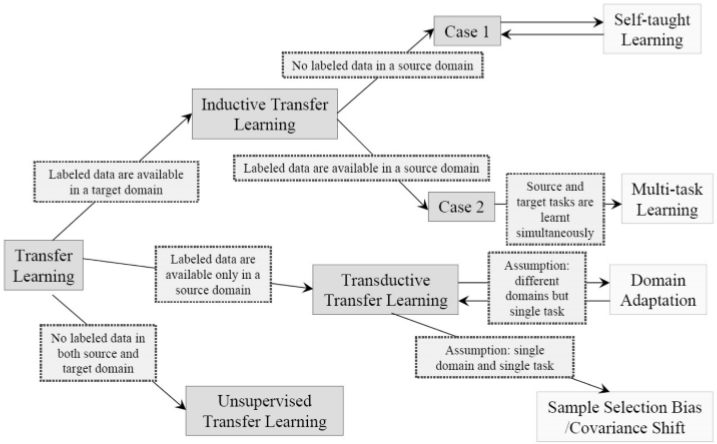
\includegraphics[width=.8\linewidth]{figures/SettingsTransferLearning.png}
	\caption[Settings of Transfer Learning]{The various settings of transfer learning approaches and there relation to traditional machine learning problems.\cite{Pan.2010}}
	\label{FigSettingsTransferLearning}
\end{figure}

\subsection{Inductive Transfer Learning}\label{TlSubSecInduc}
The setting \ac{ITL} takes the assumption that the target task and the source task are different regardless of whether the source and target domains are different or not.
Methods of this setting requiring some labelled test data to \textit{induce} a predictive model $f_\mathcal{X}(\mathbf{X})$ for the training domain.\cite{Pan.2010}
Therefore Pan et al. formulated the following definitions.
\begin{mDef}[Inductive Transfer learning {\cite{Pan.2010}}]\label{DefITL}
	 Given a source domain $\mathcal{Z}$ and a learning task $\mathcal{T_Z}$, a target domain $\mathcal{X}$ and a learning task $\mathcal{T_X}$, inductive transfer learning aims to help improve the learning of the target predictive function $f_\mathcal{X}(\cdot)$ in $\mathcal{X}$ using the knowledge in $\mathcal{Z}$ and $\mathcal{T_Z}$, where $\mathcal{T_Z} \neq \mathcal{T_X}$, while some labeled target domain data is available.
\end{mDef} 
With this in mind, there are in fact two special cases to consider.
The first one tries to achieve high performance in the target task by requiring not only some labelled test data but lots of labelled training data.
This is related to the multi-task learning approach where a learner tries to learn both domains, the source and target domain simultaneously.\cite{Pan.2010}\\
In the second case, there are no labelled source data at all available.
The goal is similar to the self-thought learning setting.
The challenge of self-thought learning is information from the source domain can not be applied to the target because they are not the same and therefore can not be used directly.
Summarizing, because the source data can not be used directly, we have to find are parts of the data which can be combined with a few labelled target data to reach the goal.\cite{Pan.2010}\\
In the section \ref{TlSubSecInstance}, we will give an example of an instance based approach, based on the inductive transfer learning setting.
Note that this solution tries to aligning the marginal distributions with some labelled data, which is little different to the original definition of inductive learning.

\subsection{Transductive Transfer Learning}\label{TlSubSecTrans}
The \ac{TTL} setting assumes that the tasks of the two domains are the same, but the source and target domains are different.
Furthermore, it requires a lot of labelled data in the source domain and assumes no labelled data in the target domain and has the requirement that some target data is available at training time.\cite{Pan.2010}
The formal definition is made with:
\begin{mDef}[Transductive Transfer Learning {\cite{Pan.2010}}]\label{DefTTL}
	 Given a source domain $\mathcal{Z}$ and a corresponding learning task $\mathcal{T_Z}$, a target domain $\mathcal{X}$ and a corresponding learning task $\mathcal{T_X}$, transductive transfer learning aims to improve the learning of the target predictive function $f_\mathcal{X}(\cdot)$ using the knowledge in $\mathcal{Z}$ and $\mathcal{T_Z}$, where $\mathcal{Z} \neq \mathcal{X}$ and $\mathcal{T_Z} = \mathcal{T_X}$.In addition, some unlabeled target domain data must be available at training time.
\end{mDef}
The term \textit{transductive} has several meanings.
In traditional machine learning, it means that \underline{all} target domain data has to be available at training time and as a consequence, the learned model cannot be reused with new, i.\,e. unseen data.
However, this can be relaxed, which the result that in the transfer learning topic \textit{transductive} means that the task must be the same and only \textit{some} unlabeled target has to be available at training time.\cite{Pan.2010}\\
The transductive setting can be divided into two special cases:
The feature spaces between the source and target data are different with $\mathcal{Z} \neq \mathcal{X}$.
This is related to the definition of heterogeneous transfer learning from \ref{TlSecHetero}.
The second case is that the feature spaces are the same, but the marginal probability distributions differ, i.\,e. $P(\mathbf{Z}) \neq P(\mathbf{X})$.\cite{Pan.2010}\\
In this case, the transductive transfer learning is related to the domain adaptation task from \ref{DefDa}.
An example of transductive transfer learning method is given in \cite{Wang.2008}.
In this, they cluster the unlabeled target data for pseudo label generation and using a custom dimension reduction with the clustered target data and the labelled source data to create a subspace.
Summarizing, because the two domains are different, transductive transfer learning aims to improve the learning by using the source data and task in combination with a few unlabeled target data.

\subsection{Unsupervised Transfer Learning}\label{TlSubSecUnsuper}
The last one, the unsupervised transfer learning section, which is obvious not part of the category supervised learning, but will be described for completeness.
It assumes that in both domains no labeled data is available.
Furthermore, the task of the source and target data are different.
In comparison with the supervised learning transfer learning methods, the goal is not to find labels for the target data but solving clustering, dimensionally reduction and density estimation.\cite{Pan.2010}
Finally, we can give the following definition.
\begin{mDef}[Unsupervised Transfer Learning {\cite{Pan.2010}}]\label{DefUTL}
	 Given a source domain $\mathcal{Z}$ with a learning task $\mathcal{T_Z}$, a target domain $\mathcal{X}$ and a corresponding learning task $\mathcal{T_X}$, unsupervised transfer learning aims to help improve the learning of the target predictive function $f_\mathcal{X}(\cdot)$ in $\mathcal{X}$ using the knowledge in $\mathcal{Z}$ and $\mathcal{T_Z}$, where $\mathcal{T_Z} \neq \mathcal{T_X}$ and $\mathcal{Y_Z}$ and $\mathcal{Y_X}$ are not observable.
\end{mDef}
Note that the predictive function $f_\mathcal{X}(\cdot)$ aims for example to find the cluster centres.
An example for Unsupervised transfer learning methods can be given from section \ref{TlSubSecHomoSymFeature} when the corresponding learner will be replaced with an unsupervised learning algorithm.
Examples are discussed in section \ref{TlSubSecHomoSymFeature}.
Summarizing, this setting aims to improve the respective tasks by the use of the source data or task.
This is, in fact, similar to the inductive transfer learning setting from section \ref{TlSubSecInduc}.\cite{Pan.2010}

\section{Homogeneous Transfer Learning}\label{TlSecHomo}
In this section, the homogeneous transfer learning approach will be introduced.
In general, it has the assumption that the feature spaces are equal and the conditional or marginal distributions of the domains are different.
There are three main goals of homogeneous transfer learning.
The first is one is to align the marginal distribution difference.
The second is to correct the difference in the conditional probability distributions, and the last one tries to align both, the marginal and conditional distribution difference.\cite[p. 6]{Weiss.2016}
This is formalised in the same way as the previous definition, which is influenced by the formulation of Pan et al. from \cite{Pan.2010}.
\begin{mDef}[Homogeneous Transfer Learning]\label{DefHomogeneous}
	Given a source domain $\mathcal{Z}$ and learning task $\mathcal{T_Z}$, a target domain $\mathcal{X}$ and learning task $\mathcal{T_T}$, homogeneous transfer learning aims to help improve the learning of the target predictive function $f_\mathcal{T}(\cdot)$ in $\mathcal{X}$ using the knowledge in $\mathcal{Z}$ and $\mathcal{T_Z}$, where $\mathcal{X_Z} = \mathcal{X_X}$ and $\mathcal{Y_Z} =\mathcal{Y_X} $, but $P(\mathbf{Z}) \neq P(\mathbf{X})$ and/or $P(\mathbf{y_\mathcal{Z}}\vert \mathbf{Z}) \neq P(\mathbf{y_\mathcal{X}}\vert \mathbf{X})$.\cite[p. 4]{Weiss.2016}
\end{mDef}
If the differences only exit in the marginal distribution, then we can build another relation to \acl{DA} from definition \ref{DefDa}.
Refer to section \ref{TlSecChal}, for examples on why the distribution can be different.\cite[p. 6-7]{Weiss.2016}\\ 
The homogeneous transfer learning category can be split up in five general approaches:
Instance-transfer, symmetric-feature transfer, asymmetric-feature transfer, parameter transfer and relational-knowledge transfer.
These approaches are sometimes called categories of information transfer.
They give a general understanding of how the methods are trying to align the differences.\cite[p. 6-7]{Weiss.2016}
Unlike the previous definitions, settings and explanations, which describing the problem and only giving an abstract solution with the predictive function.
\subsection{Instance-transfer}\label{TlSubSecInstance}
The instance transfer method tries to full fill the goal of aligning the marginal distribution by reweighting some source data.
This reweighted data is then directly used with target data for training.
It seems that these type of algorithm works best when the conditional probability is the same in source and target domain \cite[p. 6]{Weiss.2016}\\
In the following, we will present such an Instance transfer algorithm.
The so-called \textit{TrAdaBoost} which is proposed by Dai et al.\cite{Pan.2010}\\
\subsubsection{TrAdaBoost}
The TrAdaBoost\footnote{\url{https://github.com/LinZhineng/transfer-learning/tree/master/tradaboost}} algorithm extends the boosting-based learning algorithm.
The Algorithm follows the instance transfer definition and assumes that the marginal probability distribution are different, but the conditional probability distribution are the same.\cite{Dai.}
It is originally proposed as two class solution, but there are extension like MsTrAdaBoost for multi-class problems.\cite{Huang.2012}\\
The main goal is to reuse some source data in the target domain.
The source data is in general considered as out-dated.
It uses a small amount of labelled target data, considered as new data, which is called same-distribution training data.
Therefore, and because of definition \ref{DefITL}, the method has an inductive setting.
This new data is then used to help to vote on the usefulness of the old training data.\cite{Dai.}\\
The filtering boosts the part of the data which is not too far away from the same-distribution training data.
The training data in general is called diff distribution-training data.
The voted part of the data is used to make the knowledge transfer.
Furthermore, the same-distribution training data and the diff-distribution training data are forming the new source data for the training.
In the corresponding article, the weighted-\acs{SVM} is used as the underlying learner.
It is rather crucial that the learner has some weighting function because the filtering is done with weighting.\cite{Dai.}\\
The TrAdaBoost algorithm has two free parameters, which is the number of iterations and the initial value of the weight vector.
Suppose the number of fixed iterations is $T$ and the unlabeled target dataset $\mathbf{X}$.
Consider $\mathbf{Z}_D$ as diff-distribution training dataset with labels of size $N$ and the same-distribution data (from the target data) with labels $\mathbf{Z}_S$ has $M$ points.
This forms the complete training set $\mathbf{Z}=\mathbf{Z}_D\cup \mathbf{Z}_S$, with $N+M$ entries and $\mathbf{\mathbf{Z}}=\{(\mathbf{z}_i,y_i))\}$, where $y_i$ is the label for the ith-data point with $y\in {0,1}$ and $x_i$ with \cite{Dai.}:
\begin{equation*}
	\mathbf{z}_i = \begin{dcases}
						\mathbf{z}_i^D, \>\>\>\> i = 1,\dots,N\\
						\mathbf{z}_i^S, \>\>\>\> i = N +1,\dots,N+M
			  	   \end{dcases}
\end{equation*}
In every iteration, the learner is trained with this training set and predicts for the training $\mathbf{Z}$, and the unlabeled target dataset $\mathbf{X}$.
Note that the label for $\mathbf{Z}_S$ is predicted, too.\cite{Dai.}\\
At this point the filtering takes place:
If a diff-distribution data point is mistakenly predicted, then it may be caused by the difference of this instance to the same-distribution training data.
When this is the case, the \textit{TrAdaBoost} algorithm reduces the weight for this data point, and therefore this point will affect the learning process less than in the current iteration.
This is done via updating the weight vector $\mathbf{w}^t=\{w_1^t,\dots,w_{N+M}^t\}$ in the $t$-th iteration with \cite{Dai.}:
\begin{equation}\label{EqTrAdaWeighting}
	w_i^t+1=\begin{dcases}
				w_i^t\beta^{\vert h_t(\mathbf{z}_i )-y_i\vert}, \>\>\>\>\>\> 1\le i \le N \\
				w_i^t\beta_t^{-\vert h_t(\mathbf{z}_i )-y_i\vert}, \>\>\> N+1\le i \le N+M
			 \end{dcases}
\end{equation}
Where $ h_t(\mathbf{x}_i )$ is the predicted label for the $i$-th data point.
Furthermore, the different betas are set to $\beta_t = \epsilon_t / (1-\epsilon_t)$, where $\epsilon_t$ is a weighted error function and $\beta= 1 / 1 + \sqrt{2\ln n/T}$.
Note that $\epsilon_t$ function value is required to be less than 0.5.\\
The $\beta$, which is multiplied with the weight for the training data, is bound by $\beta^{\vert h_t(\mathbf{x}_i )-y_i\vert} \in (0,1]$.
After the $T$ iteration, the algorithm creates the final hypothesis of the labels based on the previous iterations.
Note that only steps which are in the range of $\{\lceil T /2 \rceil,\dots,T\}$ are considered.\cite{Dai.}\\
The error bound of the \textit{TrAdaBoost} are similar to the underlying \textit{AdaBoost}.
Furthermore, the error rate of the same-distribution data for the final hypothesis (final label assignment based on the T iterations) can be upper bounded with.
\begin{equation}
	\epsilon \le 2^{\lceil T / 2\rceil} \prod_{t=\lceil T / 2\rceil}^{T} \sqrt{\epsilon_t(1-\epsilon_t)}
\end{equation}
At this point, the required $\epsilon_t < 0.5$ becomes important.
If so, then the final error will be increasingly smaller after each iteration.\cite{Dai.}

\subsection{Symmetric-Feature-Transfer}\label{TlSubSecHomoSymFeature}
The solutions, which implementing the symmetric feature transfer are trying to find a common latent subspace for source and target domain, with the goal to reduce the marginal distribution differences.
In the subspace, they should preserve the underlying structure of the data, which can be any relation in between the data.
An example of a symmetric feature space transfer method is \ac{TCA}, which will be discussed in the following.\cite[p. 6]{Weiss.2016}
\subsubsection{Transfer Component Analysis}
The \acs{TCA} method is presented by Pan et al. in \cite{Pan.2011}\footnote{\url{https://github.com/LinZhineng/transfer-learning/tree/master/tca}}.
The authors proposed \acs{TCA} to support classifier for unsupervised and semi-supervised learning.\cite{Pan.2011}
However, the resulting kernel and the transformation matrix can be used to train a kernel based learner like the \acs{SVM}, which is in fact supervised.
It has the assumption, which makes it a homogeneous transfer method that the feature space is the same, the conditional probabilities are similar, but the marginal probability distribution are different.
Furthermore they assume that there exists a feature transformation $\phi$, which can align the differences, i.\,e. $P(\phi(\mathbf{Z})) \approx(\phi(\mathbf{X}))$ and preserve $P(\mathbf{y}_\mathcal{Z}\vert \phi(\mathbf{Z}))\approx P(\mathbf{y}_\mathcal{X}\vert \phi(\mathbf{X}))$.\cite{Pan.2011}\\
In the following we will see that \acs{TCA} requires target data in the training process and is therefore transductive.\\
In general there may exits underlying data structures and relationships in between them.
Some of them do cause the distribution difference, and some of them are the reason for relations between the source and target domain.
The part of the data which causes the relation is called \textit{transfer component} and should be found to preserve structure but at the same time aligning the differences.\cite{Pan.2011}\\
Consider $\mathbf{K}$ as a cross-domain kernel, as a composition of the source and target domain, in the embedded subspace which has the form:\cite{Pan.2011}
\begin{equation}\label{EqTCAKernel}
\mathbf{K} = 
	\begin{bmatrix}
	K_{\mathcal{Z}}\>\>\>\> K_{\mathcal{ZX}} \\
	K_{\mathcal{XZ}}\>\>\>\> K_{\mathcal{XX}}
	\end{bmatrix}
\end{equation}
Where $\mathbf{K} \in \mathbb{R}$ with size $N\times N = (N_\mathcal{Z} + N_\mathcal{X}) \times (N_\mathcal{Z}+ N_\mathcal{X})$.
This is the kernel over all data points and should be learned in a way that the marginal distribution in the subspace is aligned and the data variance (preserve data structure) is maximized.
For that the \acs{MMD} from section \ref{TlSubSecMMD} is rewritten as $tr(\mathbf{KM})$.
Where $\mathbf{M}$ is the \acs{MMD} matrix as:\cite{Pan.2011}
\begin{equation}\label{EqTCAMMD}
(M)_{ij}= \begin{dcases}
\frac{1}{N_\mathcal{Z}^2},\>\>\> \mathbf{x_i},\mathbf{x_j} \in \mathcal{Z}\\
\frac{1}{N_\mathcal{X}^2},\>\>\> \mathbf{x_i},\mathbf{x_j} \in \mathcal{X}\\
\frac{-1}{N_\mathcal{Z}N_\mathcal{X}},\>\>\> otherwise
\end{dcases}
\end{equation}
This is, in fact, the same transformation matrix for integrating \acs{MMD} as it is done by an asymmetric approach described in section \ref{TlSubSecHomoAsymFeature}.
The objective function of the \acs{TCA}, uses the \ac{MMDE} from Pans previous work from\cite{Pan.2008}. The following optimization problem is designed to align the differences of the distributions but maximizes the subspace variance:\cite{Pan.2011}
\begin{equation}\label{EqTCAReducedOpt}
\begin{gathered}
\min_{\mathbf{W}}  tr(\mathbf{W}^T\mathbf{KMKW}) + \lambda tr(\mathbf{W}^T\mathbf{W})\\
s.t. \mathbf{W}^T\mathbf{KHKW} = \mathbf{I}_{N \times N}
\end{gathered}
\end{equation}
With this, the \acs{MMDE} is simply the extensions of the \acl{MMD} with a regularization term, which can be seen on the right side of equation \eqref{EqTCAReducedOpt}.\cite{Pan.2011}\\
The parameter $\lambda \ge 0$ is a trade off parameter and the matrix $\mathbf{W} \in \mathbb{R}^{N\times L}$ does the subspace transformation.\cite{Pan.2011},\\
Note the the centering matrix $\mathbf{H} = \mathbf{I}_{N\times N} - (1/N)\mathbf{1}_{(N\times N)})$ in the constrains. Because of the centering transformation the maximized variance matrix $\mathbf{W}^T\mathbf{KHKW}$ should be persevered as identity matrix.\\
However, this seems that the kernel from equation \eqref{EqTCAKernel} is expensive to calculate via a \ac{SDP}.\cite{Pan.2011}\\
A \acs{SDP} is an extension of a linear optimisation problem, where the non-negative constrained is replaced with $\mathbf{K}\succeq 0$, which is the \acs{PSD} attribute of the Matrix. Additionally, the vector space for linear problems $\mathbb{R}^N$ is replaced with the vector space of symmetric $N\times N$ matrices based on the linear transformation of matrices.\cite{Gartner.2012}\\
For determining $\mathbf{W}$, they are ended up by formulating the optimization problem as eigenvalue problem.
By finding the largest $L$ eigenvectors with $(\mathbf{KMK}+\lambda \mathbf{I})^{-1} \mathbf{KHK}$, the subspace kernel $\mathbf{K}$ can be calculated, or the source and target data can be reduced with $\mathbf{W} \in \mathbb{R}^{N\times L}$.
The computational complexity is given by $\mathcal{O}(L(N_\mathcal{Z}+N_\mathcal{X})^2)$, where again $L$ is the number of eigenvectors.\cite{Pan.2011}
\subsubsection{Geodesic Flow Kernel}
\begin{figure}[t]
	\centering
	\floatbox[{\capbeside\thisfloatsetup{capbesideposition={right,top},capbesidewidth=5cm}}]{figure}[\FBwidth]
	{\caption[Summary of Geodesic Flow Kernel Approach]{The geodesic flow with the start and endpoints from source and target data and the induced kernel.\cite{Gong.}}}
	{\includegraphics[width=\linewidth]{figures/GFKApproach.png}\label{FigGFKApproach}}
\end{figure}
Another symmetric feature transfer method is the \ac{GFK} and is proposed by Gong et al. in \cite{Gong.}\footnote{\url{http://www-scf.usc.edu/~boqinggo/domain\_adaptation/GFK\_v1.zip}}.
Following definition of homogeneous methods and similar to \acs{TCA}, the \acl{GFK} is trying to lower the marginal distribution differences.\cite[p. 13]{Weiss.2016}\\
Furthermore, it is calimed as unsupervised transfer learning method, but because the results of this method is, in fact, a kernel, it can be trained with a kernel machine.\cite{Gong.}
Again because it needs target data in the learning process, it will be considered as inductive transfer learning method.\\
The idea of \acs{GFK} can be summarized in the following steps:
The source and the target data has to be embedded in a Grassmann manifold.
Consider a subspace $\mathcal{P} \in \mathbb{R}^{N \times d}$ with $N$ observations (dimensionality of the data) and $d$ is the feature space dimension.
Then the collection of the $d$ dimensional subspaces are forming the Grassmannian $\mathbb{G}(d, N)$ in the original $N$ dimensional feature space.\cite{Gong.}\\
Next, construct a geodesic flow and merge source (start) and target (end) data as points on the flow.
Proceed by integrating an infinite number of subspaces from start to end along the flow $\boldsymbol{\Phi}(t)$.\cite{Gong.}\\
After that, the raw features $\mathbf{x}$ are projected into the subspaces, which makes them infinite dimensional feature vectors $\mathbf{z}^\infty \in \mathcal{H}^\infty$.
The inner product will be applied over the vectors $\mathbf{z}^\infty$ to define a kernel function, which can be computed in the original feature space(kernel trick).
The kernel in the space $\mathcal{H}^\infty$ should then encapsulate the underlying difference and commonness of the source and target data.\cite{Gong.} The approach is summarised in figure \ref{FigGFKApproach}\\
For more details please have a look in the thesis \cite[p. 45;110-113]{Gong.2015} and the article \cite{Gong.}.
\subsection{Asymmetric-Feature-Transfer}\label{TlSubSecHomoAsymFeature}
The asymmetric feature transfer learning approach tries to transform the source domain data in the target (subspace) domain.
This should be done in a way that the transformed source data will match the target distribution.
In comparison to the symmetric feature transfer approaches, there will be no shared subspace, but only the target space.
In the following, the \ac{JDA} algorithm is described to give an idea of an asymmetric approach.\cite[p. 6; 10]{Weiss.2016}
\subsubsection{Joint Distribution Adaptation}
The \acl{JDA} algorithm tries to not only solve the marginal probability distribution but the conditional probability distribution, too.
This solution is proposed by Long et al. in \cite{Long.}.\footnote{\url{http://ise.thss.tsinghua.edu.cn/~mlong/doc/joint-distribution-adaptation-iccv13.zip}}\\
Because it solves the probabilistic differences between the domains, it can be considered as transductive setting, with the need for unlabeled target data.\\
The primary goal is to alter the joint distribution by a feature transformation in a way that the joint expectations of the source and target features are matched between the domains.
However, this solution for this problem is assumed as non-trivial.\cite{Long.}\\
They approximate it by searching an adaptation matrix $\mathbf{A} \in \mathbb{R}^{K \times N_\mathcal{X} }$, which can transform any new data in the subspace and is, in fact, an orthogonal transformation matrix.
Furthermore, the embedded data matrix $\mathbf{Z} \in \mathbb{R}^{N\mathcal{Z}\times K}$ is searched to transform the already existing data in the subspace.\cite{Long.}\\
This approach consists of the four steps, which are feature transformation, marginal distribution adaptation, conditional distribution adaptation and solving the resulting optimization problem.\cite{Long.}\\
Revisiting our transfer learning definition, source and target data can be represented as data matrix $T = [\mathbf{Z};\mathbf{X}] \in \mathbf{R}^{N\times M}$ where $N = N_\mathcal{Z}+N_\mathcal{X}$, with the number of source and target data respectively.
In fact, the optimization problem to solve the marginal differences are very similar to the \acs{TCA} solution from equation \eqref{EqTCAReducedOpt}.\cite{Pan.2011}\\
It seems that adopting the conditional probability distribution is a kind of bigger problem.
Since the goal is to be able to solve the transfer problem without labelled target data the $P(\mathbf{y}_\mathcal{X}\vert \mathbf{X})$ cannot be directly modeled or estimated with some statistics like it is done by the marginal adaptation.\cite{Long.}\\
Because of this, they applied a pseudo label technique.
This is done by applying a base classifier, e.\,g. \acs{SVM} to predict the not 'final' class labels for the target domain, which are the pseudo labels.
Since $P(\mathbf{y}_\mathcal{X}\vert \mathbf{X})$ is unknown, the class conditional probability functions in form of $P(\mathbf{X}\vert \mathbf{y}_\mathcal{X}=c)$(true class labels) and $P(\mathbf{X}\vert \mathbf{y}_\mathcal{X}=c)$(pseudo labels) are matched.
Here $c$ represents the classes of the label space $\mathcal{Y}$, i.\,e. $c\in{1,\dots,C}$ for $C$ labels.\cite{Long.}\\
By incorporating the class conditional distribution in the \acl{MMD}, not the sample means, but the distance between the class conditional distributions are measured:\cite{Long.}
\begin{equation}\label{EqJDAConditionalOpt}
\bigg|\bigg| \frac{1}{N_\mathcal{Z}^{(c)}} \sum_{\mathbf{x}_i \in \mathcal{Z}^{(c)}}^{N_\mathcal{Z}^{(c)}}\mathbf{A}\mathbf{x}_i^T- \frac{1}{N_\mathcal{X}^{(c)}} \sum_{\mathbf{x}_j \in \mathcal{X}^{(c)}}^{N_\mathcal{X}^{(c)}}\mathbf{A}\mathbf{x}_j^T \bigg|\bigg|^2 = \min_{\mathbf{A}^T\mathbf{A}} tr(\mathbf{A}\mathbf{X}^T\mathbf{M}_c\mathbf{X}\mathbf{A}^T)
\end{equation}
With  $\mathcal{Z}^{(c)}$ as the set of examples belonging to class $c$ in the source data, where the points are having the true class labels and $N_\mathcal{Z}^{(c)} = \vert\mathcal{Z}^{(c)}\vert$ is the size of the set.
The same applies to the target domain but with pseudo labels in $\mathcal{X}^{(c)}$ and size $N_\mathcal{X}^{(c)} = \vert\mathcal{X}^{(c)}\vert$.
The elements of the $\mathbf{M}_c$ with the use of the class labels are computed by: \cite{Long.}
\begin{equation}\label{EqJDAMMDPseudoMatrix}
(M_c)_{ij}= \begin{dcases}
\frac{1}{N_\mathcal{Z}^{(c)} N_\mathcal{Z}^{(c)} },\>\>\> \mathbf{x_i},\mathbf{x_i} \in \mathcal{Z}^{(c)} \\
\frac{1}{N_\mathcal{X}^{(c)}  N_\mathcal{X}^{(c)}  },\>\>\> \mathbf{x_i},\mathbf{x_i} \in \mathcal{X}^{(c)} \\
\frac{-1}{N_\mathcal{Z} ^{(c)} N_\mathcal{X} ^{(c)} }, \begin{cases}
\mathbf{x_i} \in \mathcal{Z}^{(c)}, \mathbf{x_j} \in \mathcal{X}^{(c)}\\
\mathbf{x_j} \in \mathcal{Z}^{(c)}, \mathbf{x_i} \in \mathcal{X}^{(c)}\\
\end{cases}\\
0,\>\>\>\>\>\>\>\> otherwise
\end{dcases}
\end{equation}
Note that because of the differences in the domains the most pseudo labels are incorrect, but it seems that in combination with the modified \acs{MMD}, it helps to draw the distribution closer together in the subspace.\cite{Long.}\\
Incorporating, they class conditional \acs{MMD} the final \acs{JDA} optimization problem is given with:\cite{Long.}
\begin{equation}\label{EqJDAMergeOpt}
\min_{\mathbf{A}\mathbf{X}^T\mathbf{M}_c\mathbf{X}\mathbf{A}^T=\mathbf{I}} \sum_{c=0}^{C} tr(\mathbf{A}\mathbf{X}^T\mathbf{M}_c\mathbf{X}\mathbf{A}^T) + \lambda \Vert\mathbf{A}\Vert^2_F
\end{equation}
Where $\lambda$ is again the regulation parameter to guarantee a distinct function for the optimization problem.\\
By analyzing this problem, they showed that solving equation \eqref{EqJDAMergeOpt} is equal by solving the eigenvalue problem of $\mathbf{X}^T\mathbf{HX}\mathbf{A}^T\boldsymbol{\Phi}$ where $\boldsymbol{\Phi} = diag(\phi_1,\dots,\phi_n)$ are the Lagrange multiplier. By finding the $K$ smallest eigenvectors for the eigenproblem of equation the transformation matrix $\mathbf{A}$ can be obtained. The embedded matrix $\mathbf{Z}$ can be obtained with $\mathbf{Z} = \mathbf{A}\mathbf{X}^T$.\cite{Long.}\\
For details to the algorithm, please refer to \cite{Long.}.
The \acs{JDA} complexity for $T\le 50$ as the number of iterations until convergence and the subspace bases with $K\le 500$ the computational complexity is given by $\mathcal{O}(TKM^2+TCN^2+TMN)$.\cite{Long.}
\subsection{Parameter-Transfer}\label{TlSubSecPara}
The third approach, the parameter transfer aims to transfer knowledge through shared parameters from source and target domains.
This is achieved by creating multiple source models, combining them and reweight them to create an improved target learner.
One approach in this category is based \ac{MMKT}.\cite[p. 7-8]{Weiss.2016}
\subsubsection{Multi Model Knowledge Transfer}
The \acs{MMKT} approach is proposed by Tommasi et al. in \cite{Tommasi.}.
They are using the \ac{LS-SVM} in combination with a discriminative method to transfer knowledge from previously learned models based on the source data and transferring it to the target data.
Note that the term models may confusing, which we will se in the following.
Furthermore, they want a classifier, which can be trained only on few training examples and being able to learn more only from few data than the standard \acs{LS-SVM} does.
The transfer knowledge method is adopted from his previous work in \cite{Tommasi.2009}.\\
Note that this method does not try to explicit minimise the distribution differences, as per definition of the homogeneous transfer learning from \ref{DefHomogeneous}.
Again, consider a labeled source dataset with $\{\mathbf{z},{y_i}\}_{i=1}^{N}$, where $y_i \in \mathcal{Y_Z} =\{1,-1\}$.
Furthermore, the feature mapping function $\phi(\cdot)$, which maps the features in the infinite space and the inducing kernel function $\mathbf{K}(\mathbf{x},\mathbf{x}')=\phi(\mathbf{x})^T\phi(\mathbf{x}')$.
Suppose that we have prior knowledge from $K$ classes (not models, but in following we will call it models), which are already trained.
This knowledge is represented with the hyperplane parameter, i.\,e. $\mathbf{w}'_j, j = \{1,\dots,K\}$, for each class.\cite{Tommasi.}\\
With that Tommasi et al. assuming that the transfer happens when the constraints of the hyperplane of the new class $K+1$ are set in a manner that it is close to the already trained classes of $K$.
Keeping this in mind, the optimization problem for the \acs{LS-SVM} can be extended to a model for multi knowledge transfer:\cite{Tommasi.}
\begin{equation}\label{EqMMKTOpt}
		\min_{\mathbf{w},b} \frac{1}{2}\Vert\mathbf{w}-\sum_{j=1}^{K}\beta_j\mathbf{w}_j'\Vert^2 + \frac{C}{2}\sum_{i=1}^{N}\zeta_i[y_i-\mathbf{w}\phi(\mathbf{x}_i)-b]^2
\end{equation}
Where $\mathbf{w}$ is searched model parameter and $C$ as free cost parameter. With $\mathbf{w}'_j$ as a parameter for the already trained model of $K$ models and $\zeta_i$ as a parameter for weighting, which helps to balance the contribution of positive and negative examples in the training data in equation \eqref{EqMMKTOpt}.
It is determined with the following chase:\cite{Tommasi.}
\begin{equation}\label{EqMMKTZeta}
	\zeta_i = \begin{cases}
			\frac{N}{2N^+}, \>\>\>\> y_i = +1,\\
			\frac{N}{2N^-}, \>\>\>\> y_i = -1
	\end{cases}
\end{equation} 
Where $N^+$ and $N^-$ representing the number of positive and negative examples of the source data, respectively.
Furthermore, the optimal solutions for $\mathbf{w}$ is now found with:\cite{Tommasi.}
\begin{equation}
	\mathbf{w} = \sum_{j=1}^{K}\beta_j\mathbf{w}_j'+\sum_{i=1}^{N}\alpha_i\phi(\mathbf{x}_i)
\end{equation}
In this the $\mathbf{w_j}'$ is weighted through $\beta_j$.
Because of the reformulated optimization problem the optimal determination of $\boldsymbol{\alpha}$ and $b$ can be expressed as:\cite{Tommasi.}
\begin{equation}\label{EqMMKTParaEst}
\begin{bmatrix}
\mathbf{K}+\frac{1}{C}\mathbf{W} \>\>\>\> \mathbf{1}\\
\mathbf{1}^T \>\>\>\>\>\>\>\>\>\>\>\>\>\> 0
\end{bmatrix}
\begin{bmatrix}
\boldsymbol{\alpha}\\
b
\end{bmatrix}
= 
\begin{bmatrix}
\mathbf{y} \\
0
\end{bmatrix}
\end{equation}
Where $\mathbf{W} = diag\{\zeta_1^{-1},\dots\zeta_N^{-1}\}$ with $\zeta_i$ as defined as \eqref{EqMMKTZeta}.\\
The $\beta_j \in (0,1)$ parameter forms $\boldsymbol{\beta} = \{\beta_1,\dots,\beta_K \}$ for controlling the degree of closeness of the new model to the $j$-th model.
Note that $\boldsymbol{\beta}$ has to be choose in the unitary ball and therefore has to be $\Vert\boldsymbol{\beta}\Vert_2\le 1$ (in the $L_2$-space).
This term is necessary to avoid overfitting problems, which happens when the number of models in comparison with the training data is large.
Furthermore, it is possible with the new model to find the optimal classes for knowledge transfer automatically.
Hence, an optimal value for $\boldsymbol{\beta}$ has to be found.\cite{Tommasi.}\\
In this method the error of the \acs{LS-SVM} is quantified with the \ac{LOO}-Error.\cite{Tommasi.}\\
The 'classical' definition of the \acs{LOO}-Error is, as the name says, leaves one data point out and creates a new 'dataset' on which a model is trained.
After that the error is calculated and is repeated as long as not all data points are already leaved out.
From the resulting errors the mean is calculated, this forms the \acl{LOO}-Error.\cite[p.74-76]{Evgeniou.2004}\\
They have incorporated this error with the \acs{LS-SVM} optimization problem and obtained the  loss function for the new approach:\cite{Tommasi.}
\begin{equation}
loss(y_i,\tilde{y}_i)= \zeta_i max[1-y_i\tilde{y}_i,0] = max \bigg[y_i\zeta_i\bigg({\mathbf{G}^{-1}_{ii}} - \sum_{j=1}^{k}\beta_j \frac{\alpha_{i(j)}'}{\mathbf{G}^{-1}_{ii}}\bigg),0\bigg]
\end{equation}
Note that $\mathbf{G}_{ii}$ and in this context means, the dataset without the $i$-th data point is applied.
Furthermore, $\tilde{y}_i$ are the \acs{LOO} predictions and $\alpha_i =\mathbf{G}_{ii}^{-1} = [\hat{y}_1^j,\dots,\hat{y}_{i-1}^j,\\\hat{y}_{i+1}^j,\dots,\hat{y}_N^j,0]^T$, with $\hat{y}_i^= \mathbf{w}'_j+\phi(x_i)$.\\
With that, the convex 'global' loss function over all models can be formulated with respect to the constrain $\Vert\boldsymbol{\beta}\Vert_2\le 1$.
This will find the optimal $\beta$'s.
In practice, the in the optimisation process is implemented with a project sub-gradient descent algorithm.\cite{Tommasi.}
The computational complexity of the algorithm is $\mathcal{O}(N^3+KN^2)$, with $N$ data points and $K$ classes, i.\,e. prior models.
\subsection{Relational-Knowledge-Transfer}\label{TlSubSecRelation}
The relational knowledge transfer aim to find some relationship between the source and target data.\cite[p. 7]{Weiss.2016}
Because the Transfer Kernel learning algorithm from section \ref{InSecTrans} finds this relationship in the eigenvalues of source and training data, we could assign this category to the method.
The details of the algorithm are discussed in this chapter because, the \acl{PCTKVM} is based on it.

\section{Heterogeneous Transfer Learning}\label{TlSecHetero}
In this section, we discuss the heterogeneous transfer learning category.
In contrast to the homogeneous transfer learning, in general, it has the assumption that the marginal distribution of the feature spaces are equal, but the feature spaces or the label space are not equal.\cite[p. 4]{Weiss.2016}\\
Keeping this in mind, the goal of the heterogeneous transfer learning methods is to align the differences in the source and target feature space.
If the marginal distribution of the domains is not the same, then further aligning steps via domain adaptation or homogeneous transfer must be done.
\cite[p. 6]{Weiss.2016}\\
We can again give the formal definition with:
\begin{mDef}[Heterogeneous Transfer Learning]
	Given a source domain $\mathcal{Z}$ and learning task $\mathcal{T_Z}$, a target domain $\mathcal{X}$ and learning task $\mathcal{T_T}$, heterogeneous transfer learning aims to help improve the learning of the target predictive function $f_\mathcal{T}(\cdot)$ in $\mathcal{X}$ using the knowledge in $\mathcal{Z}$ and $\mathcal{T_Z}$, where $P(\mathbf{Z}) = P(\mathbf{X})$, but $\mathcal{X_Z} \neq \mathcal{X_X}$ and $\mathcal{Y_Z} \neq \mathcal{Y_X} $.\cite[p. 4]{Weiss.2016}
\end{mDef}
Because the examples in challenges, section \ref{TlSecChal}, may not covering the heterogeneous definition, we will give an example in the following.
Imagine a machine learning application of software module defect classification, where a learner is trained to predict whether a software module works well or is defect prone.
Furthermore, there exists a metric for every software module, which measures, e.\,g. some performance criteria.
This forms the feature space.
If the model is trained on one software with the metric $\mathcal{X_Z}$ which has $M$ metrics and the prediction should be done for a different software which is reviewed on metric $\mathcal{X_X}$ and $N$ metrics, then it is a heterogeneous transfer problem.\cite[p 3-4]{Weiss.2016}\\
Again, there is a distinction between asymmetric and symmetric feature space transformations.
The first approach category aims to transfer the source domain in the target domain to align the differences.
Solutions from the second category, are trying to find a common latent feature space where the differences of the feature spaces are aligned.\cite[p. 19]{Weiss.2016}\\
However, because this work focuses on supervised homogeneous transfer, we will not go into more detail about the heterogeneous transfer categories, but present an example in the following to get an idea of how it works.\\
\subsubsection{Text to Image Transfer}
The \acs{TTI} method is presented by Qi et al. in \cite{Qi.2011}.
It is considered as symmetric transfer, and it can be regarded as domain depended image classification with a text extension and is, therefore, no general solution.\cite[p. 22]{Weiss.2016}
This is caused by the fact that \ac{TTI} transforms both the text data (source domain) and image data (target domain) into a latent feature space called \textit{topic space}, as we will see in the following.\\
However, first, the general motivation of the authors is explained.
Note that in the previous transfer learning methods the source and target domains, where separated by learning the source domain and evaluating at the target domain.
This is not the case with \acs{TTI} because source and target are just symbolic for two domains, which should be merged (transformed), to improve the accuracy in the arget domain.
However, the method requires target domain data.\cite{Qi.2011}\\
In general, image classification suffers from a few problems.
For example, the semantic gap between image datasets and labels are often higher than by text sets.
This is caused by the fact that text features to labels are often better to interpret in comparison with image features to labels.\cite{Qi.2011}\\
There are various websites and social networks, which have images linked to the text.
This text can be used to increase the amount of target data (images) when this text can be transformed and used for image classification.
They are using these co-occurrences (Image linked to a text; text is linked to a category) to build a semantic bridge from text to images.
This bridge can further be used to transfer semantic of text into images.\cite{Qi.2011}\\
Revisiting the previous notation from \ref{TlSecDef}, we can formulate the source (text) domain as $\mathcal{Z}$, where the samples are $\mathbf{Z} \in \mathbb{R}^{N_S\times A}$ or a single document as $\mathbf{z_i}\in \mathbb{R}^A$, with $A$ as a number of feature space dimensions.
Furthermore the target (image) domain as $\mathcal{X}$, with sample matrix $\mathbf{X} \in \mathbb{R}^{N_X\times B}$ or a single image with $\mathbf{x_i}\in\mathbb{R}^B$.
However, with the have the assumption, that the size of images set is much smaller than the size of the text set.\cite{Qi.2011}\\
The linkage through the co-occurrence of text and image is then formalized with $\mathcal{C} = \big\{\big( \mathbf{\expP{z}}_k,\mathbf{\expP{x}}_l,c( \mathbf{\expP{z}}_k,\mathbf{\expP{x}}_l) \big)\big\}$.
This means that $\mathbf{\expP{z}}_k$ is the corresponding text feature vector to an image feature vector $\mathbf{\expP{x}}_l$.
Note that in the following $c(\cdot)$ is abbreviated with $c_{k,l}$.
Through the linkage function, they build a semantic bridge from text to image.\cite{Qi.2011}\\
The so called \textit{translator} function with $T : \mathbb{R}^A \times \mathbb{R}^B \to \mathbb{R}$ weights the linkage strength between a document and image.
Now the label for an image is found with:\cite{Qi.2011}
\begin{equation}
	f_T (\mathbf{x}) = \sum_{i=1}^{N_S} y_i T(\mathbf{z}_i,\mathbf{x})
\end{equation}
Where $y_i$ is the text document label and     $f_T (\mathbf{x})$ provides the label depending on the sign.\\
The objective proposed by Qi et al. is to learn the function $T$, which maximizes the classification accuracy or rather minimizes a loss function. However, they determine $T$ by finding a transformation matrix to transfer text and images in the $P$ dimensional topic space. This means that they aggregate the data into the least $P$ topics, where the linkage strength of image and text co-occurrence is weighted. The extended $T$ function has the form of:\cite{Qi.2011}
\begin{equation}
T(\mathbf{z}_i\mathbf{x}_j) = \langle \mathbf{W}_\mathcal{Z}\mathbf{z}_i,\mathbf{W}_\mathcal{X}\mathbf{x}_i\rangle = \mathbf{z}_i \mathbf{W}_\mathcal{Z}\mathbf{W}_\mathcal{X}^T\mathbf{x}_i^T = \mathbf{z}_i\mathbf{S}\mathbf{x}_i^T 
\end{equation}
With $\mathbf{S} = \mathbf{W}_\mathcal{Z}\mathbf{W}_\mathcal{X}^T$ and size $A \times B$ and $\mathbf{W}_\mathcal{Z}$ and $\mathbf{W}_\mathcal{X}$ are the transformation matrices respectively.
In the following it is sufficient to just learn $\mathbf{S}$ rather than the transformation matrices and has to be determined in order to minimize the loss function for the prediction accuracy. This is done by the following minimization problem:
\begin{equation}\label{EqTTIGeneralOpt}
\min_{S} \gamma \sum_{j=1}^{N_T}\mathit{l}\big( y_j \cdot f_T(\mathbf{x}_j) \big) + \lambda \sum_{C}  \chi \big( c_{k,l} \cdot T(\mathbf{\expP{z}}_k,\mathbf{\expP{x}}_l)\big) + \Vert \mathbf{S}\Vert_\Sigma
\end{equation}
Note that $y_j$, in this case, is the image label.
The parameter $\gamma$ and $\lambda$ controlling the relative importance of the auxiliary data and the co-occurrence data respectively.
Furthermore, $C$ is the number of weighted co-occurrences.\\
With equation \eqref{EqTTIGeneralOpt} the general performance of the translation process is measured and can be divided into three parts.\\
The first is the empirical loss of the prediction, based on the function $f_T$.\cite{Qi.2011}
For the loss, they use the logistic loss function with $l = \log\{1+\exp(-z) \}$.\\
The second is sum over the $C$ weighted co-occurrences $c_{k,l}$ with a monotonic exponential decreasing function $\chi = \exp(-z)$.
They pretend with this choice, the optimization problem is closed-form and is easy to optimize.\\
The last term is for regulating the learning of the translator for an improved generalization ability.
They incorporating the Frobenius norm, which can be found here \cite{Ma.1994}, and the trace norm, for example defined in \cite{Rennie.2005}, to formulate a regularization term:\cite{Qi.2011}
\begin{equation}\label{EqTTITrace}
\Vert \mathbf{S}\Vert_\Sigma = \inf_{\mathbf{S} = \mathbf{W}_\mathcal{Z} \mathbf{W}_\mathcal{X}^T} \frac{1}{2}\bigg(\Vert\mathbf{W}_\mathcal{Z}\Vert_F^2 + \Vert\mathbf{W}_\mathcal{X}\Vert_F^2 \bigg) = \Omega(T)
\end{equation}
Where $\Vert \cdot \Vert_F^2$ is the Frobenius norm and $\Vert \mathbf{S}\Vert_\Sigma$ the trace norm.\\
With that, they found that the trace norm of $\mathbf{S}$ is a convex function and can be computed by a \acl{SDP}.
They argue that by minimizing equation \eqref{EqTTIGeneralOpt}, the found $\mathbf{S}$ will give a minimum of topics, used to explain the correspondence between text and image.
For finding the optimum, they used a proximal gradient method to find an approximation of the optimal solution.
For further information about the algorithm, the reader may consider \cite{Qi.2011}.

\section{Negative Transfer}\label{TlSecNeg}
A major key assumption of transfer learning is that the source and target domains are related to each other.
This is pointed out in the examples from section \ref{TlSecChal}.\\
If this assumption, however, does not hold and the domains may not relate, then the transfer learning solution can impact the performance of the underlying classifier for the target data in a negative way.\cite[p. 29]{Weiss.2016}\\
The problem is that all methods take the assumption that a relation exists, but there is no current way to determine whether a relationship exists or not.\cite[p. 1672]{Taylor.2009}
This is also shown in the dataset description in chapter \ref{EmChap}, where the datasets are designed in a way that the domains are related to each other.
However, as pointed out in the chapter, this selection of datasets is common in transfer learning community and may not consider the fact of negative transfer.
However, the negative transfer is a phenomenon that exits, which is seen in the results of sections \ref{EmSecOneData} and \ref{EmSecMulDa}, where the transfer learning methods are worse than the baseline classifier.

\section{Conclusion}
It is again worth to mention that there are not only many relationships among the definitions, but in the solutions too, refer to section \ref{TlSecHomo}.
Weiss et al. pointed out that there are many inconsistencies in the definition of transfer learning.\cite[p. 5-6]{Weiss.2016}
However, fair enough, many of the definitions are useful to distinguish how the transfer is done.
For example, is labeled target data or any target data at all needed, or how much source data has to be available, for the transfer.
In our opinion, this is crucial information to know, because it changes on how datasets have to be prepared, to make a comparison among different solutions.
Furthermore, one has to additional manual label target data before an inductive solution can be used.
Therefore the mentioned definition of inductive transfer \ref{DefITL} and transductive transfer \ref{DefTTL} are solid extension to the homogeneous \ref{TlSecHomo} and heterogeneous \ref{TlSecHetero} transfer learning definitions.\\
In contrast to the mentioned survey papers of \cite{Weiss.2016} and \cite{Pan.2010}, we choose to dive into the transfer learning methods in detail, to get an idea of how the general problem is formulated.
Furthermore, the process of how they get a solution for the problem is described, instead of giving a high-level description.
This seems reasonable, because of the already pointed out relations among the solutions, which does not omit the need for further research, give a generalized understanding of how the transfer problem can be solved.\\
Another point worth mention is that the provided solutions are proposed to support only certain learning approaches and varying between supervised, semi-supervised and unsupervised.
However, as seen in this chapter, the output of the solutions is often a kernel, transformation or embedding matrices, which can be used with any kernel-based algorithm.
Nevertheless, to be careful, for example from \cite{Long.}, \cite{Long.2015} \cite{Gong.} appears that their solutions can be easily applied to any standard classifier.\\
In practice, a classifier may have dependencies in their algorithm, and the integration is a more challenging problem.
This is might the reason that in \cite{Gong.}, they are using their implementation of $k$-nearest neighbor or that only the LibSVM, which supports pre-calculated kernels, is utilized in the corresponding articles of a transfer learning solution. 
Therefore the integration into a kernel machine may need further investigation.
In this chapter are various transfer learning definitions and methods discussed.
\chapter{Integration of Transfer Learning}\label{In}
In this chapter, two versions of the \ac{PCTKVM} are proposed.
The \acs{PCTKVM} which handles the $\theta$ as a fixed parameter and the \acs{PCTKVM}\textsubscript{$\theta$Est}, which does a theta estimation.
The extensions 'TK' to original term \acs{PCVM} should indicate the new Kernel approach to address the transfer learning problem.
As already mentioned in \ref{Tl} there are various solutions to solve the transfer learning problem.
Revisiting section \ref{TlSecHomo}, the homogeneous transfer learning problem can be summarized in four approaches: Instance-Transfer, Symmetric-Feature-Transfer, Asymmetric-Feature-Transfer, and Relational-Knowledge-Transfer.\newline
However, Long et al. in \cite{Long.2015} proposed the transfer kernel learning as another approach-category.
Nevertheless, the relational knowledge approach, transfers information through relationships between the source and target data, the \acs{TKL} approach suits well in this category.
Furthermore, because it needs target data for the learning process and according to the definition of transductive transfer learning, it can be categorized as transductive transfer setting.\\
The main idea of it is to approximate the kernel of the training set with the kernel of the test set via the Nyström kernel approximation.\cite{Long.2015}
On the other hand \cite{Schleif.2015}, proposed a \acs{PCVM} with linear costs which is also achieved via the Nyström approximation.
Therefore it seems reasonable, to integrate another interpretation of the Nyström approximation into the \acs{PCVM}.\\
Another advantage is that \acs{TKL} is very simple when it comes to dataset usage.
According to \ref{TlSecDef} there are transfer learning solutions which need pre-labeled test data.
As we will see in the following, the \acs{TKL} using only the training and test dataset as it is to compute the transfer kernel and therefore has an 'easy' handling.\newline
However, before going into the approach itself, the underlying technique should be discussed.
See section \ref{EmSubSecKernel} for details to kernels and the Gram matrix.
\section{Nyström Approximation}\label{InSecNysMeth}
The main Problem by computing eigenvalues and eigenvectors is that optimal eigenvalue decomposition has a time complexity of $\mathcal{O}(N^3)$ and alternative approaches must be found.
The Nyström Method was originally made for solving the eigenvalue equation, which can be seen in equation \eqref{EqEigsEq}.\cite{Zhang.2008}\\
It is done by selecting $N$ randomly observations (rows/columns) without replacement of $\mathbf{K}$ for calculating the approximation.\cite{Williams.2000}
Considering a symmetric positive semi definite kernel $k(\mathbf{z},\mathbf{x})$ which satisfies Mercers Theorem, then $\mathbf{K}$ has the following properties and can be represented as:\cite{Williams.2000}
\begin{equation}\label{EqKernelRep}
	k(\mathbf{z},\mathbf{x}) = \sum_{i=1}^{D}\lambda_i\phi_i(\mathbf{z})\phi_i(\mathbf{x}) 
\end{equation}
With $D < \infty$ as the number of feature space dimensions and $\lambda_1 \ge \lambda_2\ge\dots\ge0$ as the sorted eigenvalues and $\phi_i$ as eigenfunctions.
As consequence of Mercer follows that  $\lambda_i$ and $\phi_i$ have to satisfy the eigenvalue equations:
 \begin{equation}\label{EqEigsEq}
	\int_{i=1}^{D} k(\mathbf{x},\mathbf{z})\phi_i(\mathbf{z})p(\mathbf{z})d\mathbf{x} = \lambda_i\phi_i(\mathbf{x})
\end{equation}
With $p(\mathbf{z})$ as the probability density of the input vector $\mathbf{z}$.
Furthermore, the orthogonality conditions are satisfied with:\cite[p. 59]{Scholkopf.2001}
\begin{equation}\label{EqEigsOrt}
	\int \phi_i(\mathbf{z})\phi_j(\mathbf{z})p(\mathbf{z})d\mathbf{z} = \delta
\end{equation}
If a kernel defined above is given, then an empirical estimate can be done by, drawing an identical and independently sample ${\mathbf{z}_1,\dots,z_N}$ from $p(\mathbf{z})$.
The integral can be rewritten as an empirical estimate:\cite{Williams.2000}
\begin{equation}\label{EqEigsEmp}
	\sum_{k=1}^{N}\frac{k(\mathbf{x},\mathbf{z}_k)\phi_i(\mathbf{z}_k)}{N} \approx \lambda_i\phi_i(\mathbf{x})
\end{equation}
Where $N$ is the number of used observation from the kernel and the $N$ eigenfunctions are still orthogonal.
If we consider the N columns from $\mathbf{K} \in \mathbb{R}^{K\times K}$ as separate kernel matrix $\mathbf{K}^{(N)}$ with size $N\times N$ and elements $K_{ij}^{(N)}=K(\mathbf{z_i,z_j})$ for $i,j=1,\dots,N$, then we can use this for the eigenvalue problem of this (smaller) kernel:\cite{Williams.2000}
\begin{equation}\label{EqEigsProb}
	\mathbf{K}^{(N)}\mathbf{U}^{(N)} = \mathbf{U}^{(N)}\mathbf{\Lambda}^{(N)}
\end{equation} 
With $\mathbf{U}^{(N)} \in \mathbb{R}^{N\times N}$ as eigenvectors and $\boldsymbol{\Lambda}^{(N)}$ as a diagonal matrix with the eigenvalues for the small kernel with $\lambda_1^{(N)}\ge\lambda_2^{(N)}\ge\dots\lambda_N^{(N)} \ge0$.
If we consider points within the kernel $K^{(N)}$, then $\mathbf{x}$ can be replaced with $\mathbf{z}_j$.
Furthermore, matching \eqref{EqEigsProb} against \eqref{EqEigsEmp} then the following approximation can be obtained:\cite{Williams.2000}
\begin{equation}\label{EqEigsFuncAprox}
	\phi_i(\mathbf{z}_j) \approx \sqrt{N}U_{ij}^{(N)}
\end{equation}
Finally, by using $\phi_i(x_k)$ in \eqref{EqEigsEmp} the approximation for the any eigenvector or eigenvalues can be given by:
\begin{equation}\label{EqEigsValAprox}
	\phi_i(\mathbf{x})\approx\frac{\sqrt{N}}{\lambda_i^{(N)}}\sum_{k=1}^{N}k(\mathbf{x},\mathbf{z_k})U_{k,i}^{(N)}, \>\>\>\>\> \lambda_i \approx \frac{\lambda_i^{(N)}}{N}
\end{equation}
With this, the $i$-th eigenfunctions and eigenvalues can be approximated by calculating the sample kernel.\cite{Williams.2000}
As a consequence the eigenfunctions and eigenvalues of the whole kernel can be approximated.
\subsection{Nyström Kernel Learning}\label{InSubSecNyKerneLearning}
Willams and Seeger extended the work of Nyström to speed up kernel machines.
The problem with kernel-based predictors, e.\,g., \acs{SVM}, is similar to the eigenvalue decomposition problem from section \ref{InSecNysMeth}
It requires the computational complexity of $\mathcal{O}(N^3$) in the worst case, with $N$ as the number of training examples, to find a solution.\cite{Williams.2000}\\
With the Nyström approximation, the complexity for predictors can be bound by $\mathcal{O}(M^3N)$ with using a smaller system with size $M$, where $M<N$.\cite{Williams.2000}\\	
Now the goal is to create a low-rank approximation Matrix $\tilde{\mathbf{K}}$ of the original $N\times N$ kernel matrix $\mathbf{K}$.
Revisiting section \ref{InSecNysMeth}, using the technique of Nyström, a kernel $\mathbf{K}$ which satisfies Mercer's theorem is needed.\cite{Williams.2000}
Furthermore, we draw $M$ \acs{IID} samples of $\mathbf{K}$ and therefore we can rewrite the symmetric kernel according to:\cite{Nemtsov.2016}
\begin{equation}\label{EqNystKernelParts}
	\mathbf{K} = 
	\begin{bmatrix}
		 \mathbf{K}_{M,M}\>\>\>\> \mathbf{K}_{M,N-M} \\
		 \mathbf{K}_{N-M,M}\>\>\>\> \mathbf{K}_{N-M,N-M}
	\end{bmatrix}
\end{equation}
Where $\mathbf{K}_{M,M}$ is the sample matrix and $\mathbf{K}_{N-M,M}$ is the submatrix of $\mathbf{K}$, which is the kernel of the sample, and the rest of the data $\mathbf{K}_{N-M,N-M}$.
Because $\mathbf{K}$ is symmetric $\mathbf{K}_{N-M,M} = (\mathbf{K}_{M,N-M})^T$.
Furthermore, $\mathbf{K}_{N-M,N-M}$ is the part of the kernel which is not sampled or 'used' for the approximation, as we will see.\\
Motivated by the general eigenvalue problem, which can be obtained from \cite[p. 221]{Hartmann.2015} and shown in \eqref{EqEigsProb}, a kernel can be approximated through another kernel $\tilde{\mathbf{K}} = \tilde{\mathbf{U}}\tilde{\mathbf{\Lambda}}\tilde{\mathbf{U}}^T=\sum_{i=1}^{p}\tilde{\lambda}_i^{(N)}\tilde{\mathbf{u}}_i^{(N)}(\tilde{\mathbf{u}}_i^{(N)})^T$.\cite{Williams.2000}
With the approximated eigenvalues and eigenvectors as $\tilde{\lambda}_i^{(N)}$ and $\tilde{\mathbf{u}}_i^{(N)}$ respectively.\\
Therefore, we proceed with the equations to approximate the eigenvalues and eigenvectors.
By applying the equations of \eqref{EqEigsFuncAprox} and \eqref{EqEigsValAprox}, the approximation is based on the eigenvalues and eigenvectors of the sample matrix can be made with:\cite{Zhang.2008}
\begin{equation}\label{EqNystEigsApprox}
	\begin{gathered}
			\tilde{\lambda}_i^{(N)} = \frac{N}{M}\lambda_i^{(M)} \>\>\>\>\> \sim \>\>\>\>\> \boldsymbol{\Lambda}^{(N)} =\frac{N}{M}\boldsymbol{\Lambda}^{(M)}\\
			\tilde{\mathbf{u}}_i^{(N)} = \sqrt{\frac{M}{N}}\frac{1}{\lambda_i^{(M)}}\mathbf{K}_{N,M}\mathbf{u}_i^{(M)}\>\>\>\>\> \sim \>\>\>\>\> \mathbf{U}^{(N)} = \sqrt{\frac{M}{N}}\mathbf{K}_{N,M}\mathbf{U}^{(M)}(\boldsymbol{\Lambda}^{(N)})^T
	\end{gathered}
\end{equation}
With $i=1,\dots,N$ and $u_i^{(M)}$ and $\lambda_i^{(M)}$ from the eigenproblem (Eq. \eqref{EqEigsProb}).
After obtaining the approximated eigenvalues and vectors, the full approximated kernel can be restored:\cite{Williams.2000}\cite{Zhang.2008}
\begin{equation}\label{EqNystKernelEigsApprox}
	\tilde{\mathbf{K}} = \bigg(\sqrt{\frac{M}{N}}\mathbf{K}_{N,M}\mathbf{U}^{(M)}(\boldsymbol{\Lambda}^{(N)})\bigg)\bigg(\frac{N}{M}\boldsymbol{\Lambda}^{(M)}\bigg)\bigg(\sqrt{\frac{M}{N}}\mathbf{K}_{N,M}\mathbf{U}^{(M)}(\boldsymbol{\Lambda}^{(N)})\bigg)^T 
\end{equation}
With the use of $\tilde{\mathbf{K}} = \tilde{\mathbf{U}}\tilde{\mathbf{\Lambda}}\tilde{\mathbf{U}}^T$ in equation \eqref{EqNystEigsApprox} the approximation can be rewritten as:
\begin{equation}\label{EqNystKernelApprox}
		\tilde{\mathbf{K}} = \mathbf{K}_{N,M}(\mathbf{K}_{M,M})^{-1}\mathbf{K}_{M,N}
\end{equation}
From \eqref{EqNystKernelApprox} one can see that the kernel approximation can fully be made by the sample matrix and the submatrix $K_{N-M, N}$ of the 'original' kernel.\cite{Williams.2000}\\
The error bound of the Nyström Kernel approximation is $E_{Nys}=||\mathbf{K}-\tilde{\mathbf{K}}||$.\cite{He.2017}
This error can be minimized by choosing the samples carefully and a reasonable amount of it.
If the original Kernel $\mathbf{K}$ has to rank $M$ and the samples are linearly independent columns from the kernel, then the approximation is exact.
As a consequence, from above choosing only $P$ samples with $P< M$ the error rises the fewer columns are chosen.\cite{Williams.2000}\\
The problem with choosing (sampling) columns/rows is that we usually do not know which columns are linearly independent.
Therefore, some sampling methods or approximations were made in the past to make this sampling more deterministic.
For example, \cite{Kumar.2012}, which tries to find good samples through various sampling techniques, or \cite{Li.2015}, where the authors are drawing a large sample but approximate the submatrices with \ac{SVD}.\\
To summarize the Nyström Kernel approximation, first, we select $P$ of $N$ 'good' samples from the data reorganizing the kernel according to \eqref{EqNystKernelParts}.
At this point, we have two options:
First calculating the kernel just for the $\mathbf{K}_{M, M}$ and the submatrix ${K}_{N-M, M}$, continuing with approximate the eigenvectors and eigenvalues and finally calculating the approximated kernel $\tilde{\mathbf{K}}$ \eqref{EqNystKernelEigsApprox}.
Second calculate the approximation directly from the kernel as shown in equation \eqref{EqNystKernelApprox}. Note that the second approach needs a matrix inversion, which should be considered for the use with large datasets.
\section{Domain Invariant Kernel Learning}\label{InSecTrans}
The \ac{TKL} approach is made by Long et al. in  \cite{Long.2015}\footnote{\url{http://ise.thss.tsinghua.edu.cn/~mlong/doc/transfer-kernel-learning-tkde15.zip}}.
They are interpreting the kernel approximation from a different point of view.
The main idea is to see the train dataset-matrix, which has to be approximated, regarding Nyström, which will be approximated by the test dataset. Proceed by finding eigenvalues in a way that the difference between the approximation and ground truth train kernel will be minimal. This forms a domain invariant kernel for transfer learning.\cite{Long.2015}
The principal process is shown in figure \ref{FigTKLApp}.\newline 
From the above consider $\mathbf{z}$ as $\mathbf{Z}=\{\mathbf{z}_1,\dots,\mathbf{z}_{N}\}$ as training dataset which is sampled from $p(\mathbf{Z})$ within training domain $\mathcal{Z}$ and $\mathbf{x}$ as $\mathbf{X}=\{\mathbf{x}_1,\dots,\mathbf{x}_{M}\}$ as test dataset sampled from $p(\mathbf{X})$ within the test domain $\mathcal{X}$.
The definitions are based on \ref{TlSecDef}.
The associated kernels are $\mathbf{K}_\mathcal{Z}$ for training and $\mathbf{K}_\mathcal{X}$ for testing.\\
A fundamental insight of the \acs{RKHS} is that any \ac{PSD} kernel can be reconstructed based on the eigensystem of it. Furthermore, any new datasets can be incorporated into a kernel.\cite{Long.2015}\\
This means given a kernel $\mathbf{K}_\mathcal{X}$ of the dataset, using only the eigensystem $\{\lambda_i,\phi_i(\mathbf{x})\}$ the kernel can be evaluated by any new data point $\mathbf{z}$ and finally generating the kernel $\mathbf{K}_\mathcal{Z}$.
Again we could approximate the needed training kernel through:\cite{Long.2015}
\begin{equation}\label{EqTrainTestApprox}
	\mathbf{K}_\mathcal{Z} \simeq \mathbf{U}_\mathcal{Z}\boldsymbol{\Lambda}_\mathcal{X} \mathbf{U}_\mathcal{Z}^T = \mathbf{K}_\mathcal{ZX}\mathbf{K}_\mathcal{X}^{-1}\mathbf{K}_\mathcal{XZ}
\end{equation}
Where $\mathbf{U}_\mathcal{Z}$ as eigenvectors of the training kernel, $\boldsymbol{\Lambda}_\mathcal{X}$ as eigenvalues of the target kernel and $\mathbf{K}_\mathcal{ZX} = \mathbf{K}_\mathcal{ZX}^T$.
This is, in fact, a rewritten version of \eqref{EqNystKernelApprox}.\\
However, there might be a major problem.
Regarding two feature spaces, especially when it comes to transfer learning, where we have taken in section \ref{TlSecDef} the assumption that test and training feature spaces following different probability distributions.
This means that $P(\mathbf{Z})\neq P(\mathbf{X})$ and as a consequence the error of the approximation from \eqref{EqTrainTestApprox} can be arbitrarily large.\cite{Long.2015}\\
However, to align the distribution difference is one goal of transfer learning.
The main improvement which is done by Long et al. is to tackle this problem and to learn the domain invariant approximated kernel $\mathbf{\expP{K}}_{\mathcal{A}}$.\cite{Long.2015}
\begin{figure}
	\centering
	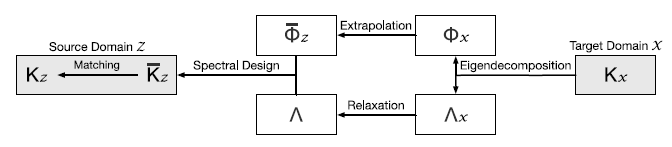
\includegraphics[width=.8\linewidth]{figures/ProcessTKL.png}
	\caption[Tranfer Kernel Learning Process]{The Process of the Domain Invariant Kernel learning. It illustrates the relaxation of eigenvalues and extrapolation of eigenvectors. \cite{Long.2015}}
	\label{FigTKLApp}
\end{figure}
\subsection{Learning Approach}\label{InSubSecLearnApp}
From a 'kernel' point of view aligning the distribution of data, where the kernel is based on, can be formulated as $P(\phi(\mathbf{z})) \simeq P(\phi(\mathbf{x}))$.\cite{Long.2015}
However, the kernel-induced feature map cannot be explicitly represented and therefore the handling of distributions in the corresponding Hilbert space is difficult.\cite{KaiZhang.2013}\\
Therefore Long et al. take the assumption that it is sufficient that $\mathbf{K}_\mathcal{Z} \simeq \mathbf{K}_\mathcal{X}$.
However, there is another problem coming up with it, because it can not be assumed that the training and test sets are equal, which means that the size of the kernels is not equal, i.\,g. $\mathbf{K}_\mathcal{Z} \in \mathbb{R}^{N\times N}$ and $\mathbf{K}_\mathcal{X} \in \mathbb{R}^{M\times M}$ with $N \neq M$.
Therefore the extrapolated source kernel $\expP{\mathbf{K}}_\mathcal{Z} \in \mathbb{R}^{N\times N}$, by using the eigensystem of the target kernel $\mathbf{K}_\mathcal{X}$. The kernel  $\expP{\mathbf{K}}_\mathcal{Z} $ will be compared to the actual training kernel $\mathbf{K}_\mathcal{Z}$.\cite{Long.2015}\\
For clarifying the terms, Long et al. proposed the term extrapolated instead of approximation regarding the Nyström approximation.\cite{Long.2015}
In this thesis, we will stick to the proposed notation to coincide.\\
The task is now to learn this extrapolated kernel, which is done step by step by first \textit{extrapolate} the eigenvectors with:\cite{Long.2015}
\begin{equation}\label{EqExtraEigs}
	\expP{\mathbf{U}}_\mathcal{Z} \simeq \mathbf{K}_\mathcal{ZX}\mathbf{U}_\mathcal{X} \boldsymbol{\Lambda}_\mathcal{X}^{-1}
\end{equation}
According to Nyström, the eigenvalues $\boldsymbol{\Lambda}_\mathcal{X}$ of the test kernel are indispensable.
However, in this approach, a \textit{relaxation} of the eigenvalues is done by considering the eigenvalues as learnable parameters $\boldsymbol{\Lambda} = diag[\lambda_1,\dots,\lambda_{M}]$.
Therefore the kernel extrapolation can be expressed as:\cite{Long.2015}
\begin{equation}
	\expP{\mathbf{K}}_\mathcal{Z} = \expP{\mathbf{U}}_\mathcal{Z} \boldsymbol{\Lambda} \expP{\mathbf{U}}_\mathcal{Z}^T
\end{equation}
With that $\boldsymbol{\Lambda}$ does not necessarily reduce the distribution difference and has to be well chosen.
This approach should preserve the original structure of the test domain while remaining flexible to solve the difference in distribution.
Another point of view is that the kernel is extrapolated from the target data but evaluated by the training data.\cite{Long.2015}\\
To construct the new kernel, Long et al. using the key knowledge from spectral kernel design:
It states that a kernel which is generated from the eigensystem of another positive semi-definite kernel, then the produced kernel will positive semi-definite itself.\cite{KaiZhang.2013}.
Therefore it seems reasonable to set $\lambda \ge 0$ to guarantee a \acs{PSD} kernel.
The error of the approximation $\expP{\mathbf{K}}_\mathcal{Z}$ to the original ground truth kernel $\mathbf{K}_\mathcal{Z}$ is determined using the squared loss, which is presented in the following:\cite{Long.2015}
\begin{equation}\label{EqTKLSquareErrorLoss}
	\begin{gathered}
		\min_{\boldsymbol{\Lambda}} || \expP{\mathbf{K}}_\mathcal{Z} - \mathbf{K}_\mathcal{Z}||^2_F = || \expP{\mathbf{U}}_\mathcal{Z} \boldsymbol{\Lambda}  \expP{\mathbf{U}}_\mathcal{Z}^T - \mathbf{K}_\mathcal{Z} ||^2_F \\
		\lambda_i \ge \zeta \lambda_{i+1}, i = 1,\dots,M-1 \\
		\lambda_i \ge 0,  i = 0,\dots,M
	\end{gathered}
\end{equation}
With $\zeta \ge 1$ is the eigenspectrum dumping factor since the eigenspectrum is power-law distributed and therefore $\zeta$ should produce larger eigenvectors.
With this, they should contribute more to the knowledge process.\cite{Long.2015}
\subsection{Learning Algorithm}\label{InSubSecLearnAlgo}
In the section above, we defined the squared error loss function for the \acs{TKL} approach.
In this subsection, we will introduce the resulting optimization problem and the \acs{TKL} algorithm in general.\\
The learning problem is convex and therefore will always find the global minimum.
Furthermore, it is a \ac{QP} with linear constraints which can be solved for example by the build in MatLab package \textit{quadprog}.
The squared loss function from \eqref{EqTKLSquareErrorLoss} is reformulated in a general matrix format and is expressed as:\cite{Long.}
\begin{equation}\label{EqTklQP}
	\begin{gathered}
		\min_{\boldsymbol{\lambda}} \boldsymbol{\lambda}^T \mathbf{Q} \boldsymbol{\lambda} - 2\mathbf{r}^T\boldsymbol{\lambda}\\
		\mathbf{C}\boldsymbol{\lambda} \ge 0 \\
		\boldsymbol{\lambda} \ge 0 \\
	\end{gathered}
\end{equation}
The inequalities representing the linear constraints.
The coefficient matrix $\mathbf{Q}$, $r$ and the constraint matrix C are defined as:
\begin{equation}\label{EqTklQPCons}
		\begin{gathered}
			\mathbf{Q} = (\expP{\mathbf{U}}_\mathcal{Z} \expP{\mathbf{U}}_\mathcal{Z}^T)\odot (\expP{\mathbf{U}}_\mathcal{Z}^T \expP{\mathbf{U}}_\mathcal{Z})\\
			r = diag[\expP{\mathbf{U}}_\mathcal{Z}^T \mathbf{K}_\mathcal{Z} \expP{\mathbf{U}}_\mathcal{Z}]\\
			\mathbf{C} = \mathbf{I} - \zeta \mathbf{I}
		\end{gathered}
\end{equation}
Where $\mathbf{I} \in \mathbb{R}^{M\times M}$ as the identity matrix and $\odot$ as Hadamard multiplication.
Note that the eigenspectrum dumping factor $\zeta$ is the only free parameter which needs to be tuned because the $\boldsymbol{\Lambda}$ is learned within the optimization problem.\\
Finally, similar to equation \ref{EqNystKernelParts}, we can reconstruct the 'joint' Kernel:\cite{Long.}
\begin{equation}\label{EqTKLKernel}
	\expP{\mathbf{K}}_\mathcal{A} = 
	\begin{bmatrix}
	 \expP{\mathbf{U}}_\mathcal{Z} \boldsymbol{\Lambda} \expP{\mathbf{U}}_\mathcal{Z}^T \>\>\>\> \expP{\mathbf{U}}_\mathcal{Z} \boldsymbol{\Lambda} \mathbf{U}_\mathcal{X}^T \\
	 \mathbf{U}_\mathcal{X} \boldsymbol{\Lambda} \expP{\mathbf{U}}_\mathcal{Z}^T \>\>\>\> \mathbf{U}_\mathcal{X} \boldsymbol{\Lambda} \mathbf{U}_\mathcal{X}^T 
	\end{bmatrix}
	= 	 \expP{\mathbf{U}}_\mathcal{A} \boldsymbol{\Lambda} \expP{\mathbf{U}}_\mathcal{A}^T 
\end{equation}
Where $\mathcal{A}= \mathbf{Z} \cup \mathbf{X}$ as one dataset for two domains.
Therefore it forms the eigenvector matrix $ \expP{\mathbf{U}}_\mathcal{A} =[ \expP{\mathbf{U}}_\mathcal{A};\>  \mathbf{U}_\mathcal{X}]$, which are the extrapolated eigenvectors of the whole dataset.\newline
The complete \acs{TKL} algorithm is summarized in algorithm \ref{PseudoCodeTKL}.\cite{Long.2015}
\begin{algorithm}
	\caption{Transfer Kernel Learning Algorithm}\label{PseudoCodeTKL}	
	\begin{algorithmic}[1]
		\Require Input Data $\mathbf{I} = [\mathbf{Z};\mathbf{X}]$; kernel(-type) $k$; eigenspectrum dumping factor $\zeta$.
		\Ensure Domain invariant kernel $\expP{\mathbf{K}}_\mathcal{A}$.
		\State Compute the kernel parts $\mathbf{K}_\mathcal{Z}$, $\mathbf{K}_\mathcal{X}$ and $\mathbf{K}_\mathcal{ZX}$ with $k$.
		\State Eigendecompose of $\mathbf{K}_\mathcal{X}$ for $\{\mathbf{\Lambda}_\mathcal{X}, \mathbf{U}_\mathcal{X}\}$ like \eqref{EqEigsProb}.
		\State Extrapolate for source eigensystem  $\expP{\mathbf{U}}_\mathcal{Z}$ with \eqref{EqExtraEigs}.
		\State Solve the \acs{QP} for eigenspectrum $\mathbf{\Lambda}$ with \eqref{EqTklQP}.
		\State Merge results and return it as \eqref{EqTKLKernel}.
	\end{algorithmic}
\end{algorithm}
The underlying kernel which is calculated in the first row of algorithm \ref{PseudoCodeTKL} is the Gaussian Kernel from \eqref{EqRBFAKernel}.\\
The process of getting the \acs{TKL} kernel is shown in figure \ref{FigKernelComparison}. In \ref{FigGaussianKernel}, in the upper left, the source set is visible.
This means that the source and target dataset is separable from each other.
After creating the \acs{TKL} kernel in \ref{FigTKLKernel}, the differences are slightly aligned.\\
The error of the approximation of the \acl{TKL} algorithm is $E_{TKL} = \Vert \expP{\mathbf{U}}_\mathcal{Z} \boldsymbol{\Lambda}\expP{\mathbf{U}}_\mathcal{Z}^T - \mathbf{K}_\mathcal{Z}\Vert$.
Furthermore, the approximation error of the Nyström kernel is bound by $E_{NystKer} = \Vert \mathbf{K}_{\mathcal{ZX}} \mathbf{K}_{\mathcal{X}}^{-1}\mathbf{K}_{\mathcal{XZ}}\Vert$.
Based on these errors, if $\boldsymbol{\Lambda} = \boldsymbol{\Lambda}_\mathcal{X}$, then the errors of $E_{NystKer}$ and $E_{TKL}$ are equal. 
However, because the $\boldsymbol{\Lambda}$ is a free parameter and the approximation error is directly minimized, the error of the \acs{TKL} approximation is bound by $E_{TKL}\le E_{NystKer}$.\cite{Long.}\\
In many real-world problems, the eigenvalues are following the power law distribution.
This means that there a few large eigenvalues and many small, in comparison with the large, eigenvalues.\cite{Mihail.2002}
Therefore it is considered as unnecessary to use the whole eigenspectrum and just compute the $R$ largest eigenvalues.
This is used to speed up the computation because the problem is greatly reduced.
The number of eigenvectors is therefore fixed to $R=min(500,M)$ and the eigenvectors can be reduced to $\expP{\mathbf{U}}_\mathcal{Z} \in \mathbb{R}^{R\times R}$ or $\mathbf{\lambda} \in \mathbb{R}^{R\times M}$.\cite{Long.}\\
The complexity of the \acs{TKL} algorithm can be given with $\mathcal{O}((D+R)(N+M)^2)$, where $R$ denotes the number of used eigenvectors, $D$ refers to the kernel.\cite{Long.}
\begin{figure}
	\centering
	\begin{subfigure}{.5\textwidth}
		\centering
		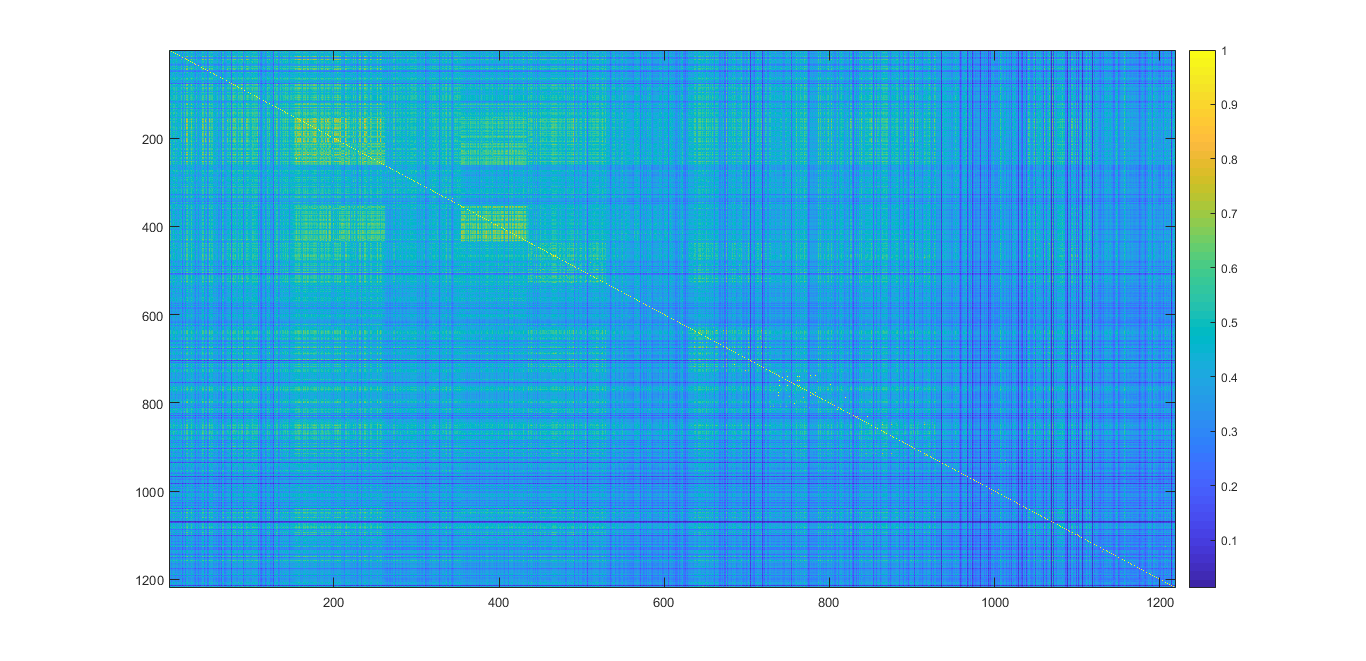
\includegraphics[width=1\linewidth]{figures/GaussianKernelIMG.png}
		\caption{Gaussian Kernel\label{FigGaussianKernel}}
	\end{subfigure}%
	\begin{subfigure}{.5\textwidth}
		\centering
		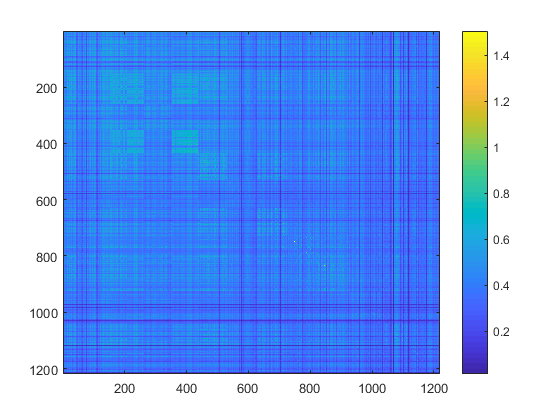
\includegraphics[width=1\linewidth]{figures/TKLKernelIMG.png}
		\caption{\acs{TKL} Kernel\label{FigTKLKernel}}
	\end{subfigure}
	\caption[Scatter Plot of TKL and Gaussian Kernel]{The scatter plot of the Gaussian and the \acs{TKL} kernel. On the left side the Gaussian kernel is shown. On the right, the \acs{TKL} kernel is shown. Is is observable that the differences of source and target sets are slightly aligned. It is based on the image set\label{FigKernelComparison}}
\end{figure}
\section{PCTKVM Algorithm}\label{InSecAlgo}
In this section, the \acl{PCTKVM} algorithm will be discussed in detail.
As shown above, we have obtained our transfer learning kernel with algorithm \ref{PseudoCodeTKL}.
According to \cite{Long.2015} the new kernel can be feed to any kernel machine.
This means that we can train the regular \acf{PCVM} with our new kernel.
To train it we are using the extrapolated training kernel which is.
\begin{equation}
	\expP{\mathbf{K}}_\mathcal{Z} = \expP{\mathbf{U}}_\mathcal{Z}\mathbf{\Lambda}\expP{\mathbf{U}}_\mathcal{Z}^T
\end{equation}
However, simply using it in algorithm \ref{PseudoCodePcvm} has some disadvantages.
Revisiting the \acs{PCVM} algorithm the kernel is recalculated in every iteration based on the optimized theta from the previous iteration.
As a consequence, we have to recalculate the entire transfer kernel too.
With the complexity of the \acs{PCVM} which is $\mathcal{O}(B^3)$ with $B$ as a number of basis functions.
We consider the worst case and substitute the number of basis function with the number of training samples $N$, which results in $\mathcal{O}(N^3)$.
The complexity of the \acs{TKL} is $\mathcal{O}((D+R)(N+M)^2)$, combining the two, we would end up with a computational complexity of $\mathcal{O}(N^3(D+R)(N+M)^2)$.
This may be resulting in a long computational time.
In fact, the question is, whether we explicitly need the theta optimization in every iteration or not.
However, one advantage of the \acs{PCVM} was, to optimize the parameters within and therefore omit the need for cross-validation.
Furthermore, the performance of the \acs{PCTKVM} depends a lot from the quality of the theta, which can be seen in figure \ref{FigPerfomanceTheta}.
To keep this advantage and the performance up, a new approach must be found.
One approach could be to optimize the theta in not every iteration.
However, this seems to be no good solution, because we have observed that the theta is just dangling around the initial value, where we optimized the theta in every 5 or 10 iterations and nevertheless was leading in our tests to a worse performance, rather than just use a fixed value for theta.
The latter option would be to set the theta to a fixed value and omit the theta optimization completely.
Fair enough we can observe a good performance, which can be seen in section \ref{EmChap}.
Furthermore, we could obtain the complexity of $\mathcal{O}(N^3+(D+R)(N+M)^2)$.
If we consider $D$ and $R$ as constant and by multiplying out, we obtain $\mathcal{O}(N^3+M^2)$ for the \acs{PCTKVM} with a fixed theta.
\begin{figure}
	\centering
	\floatbox[{\capbeside\thisfloatsetup{capbesideposition={right,top},capbesidewidth=6.5cm}}]{figure}[\FBwidth]
	{\caption[Perfomance in Dependence of Theta]{The performance of the \acs{PCTKVM} algorithm for different thetas shown as accuracy in \%, evaluated at the Reuters dataset.}}
	{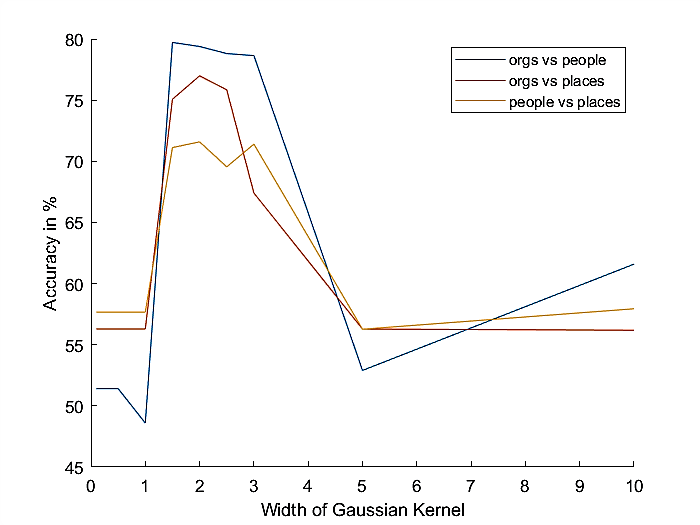
\includegraphics[width=\linewidth]{figures/PerformanceGaussianKernel.png}\label{FigPerfomanceTheta}}
\end{figure}
\FloatBarrier
\subsection{Theta Estimation}\label{InSubSecTheta}
Another, more deterministic but heuristic, approach to obtain a theta is presented by Kitayama in \cite{Kitayama.2011} and is discussed in the following.\\
It is important to notice that is just a simple estimation and therefore the optimal theta may not be found with this approach.\\
The width of the Gaussian kernel can play an important role not only for the \acs{PCVM} but many other algorithms.
Defining a 'good' value for the width leads to a more useful function which is observable in figure \ref{FigGaussianWidthRegression}.\cite{Kitayama.2011}
In this the black dots representing the data, the dashed lines are the Gaussian kernel, and the solid lines represent the regression.
In  \ref{FigSmallWidth} the width is set to 0.5 and in \ref{FigLargeWidth} it is set to 1.\newline
They are claiming in general that solving the theta via an optimization problem is very time-consuming.
The reason for this is because the optimization problem is depending on the data function, which can give a very large amount of variables and purposed a simpler algorithm to find a good $\theta$.\cite{Kitayama.2011}\\
First, they use a scaling technique to scale every dimension to an equal range.
Consider $K = N + M$ as the number of all samples with $D$ dimensions.
In the approach, they using a \textit{Min-Max} Normalization to do it.\cite{Kitayama.2011}
\begin{equation}
	x_j = \frac{x_j - x_j^L}{x_j^U-x_j^L} \times s, \>\>\> i=1,\dots,D 
\end{equation}
Where $x_j^L$ is the lower bound and $x_j^U$ is the upper bound of value and $s=\alpha\times s \alpha \ge 0$.
The $s$ is the abort criterion, but not needed in our approach.
The author's recommendation is to set alpha to 1.1.
Moreover, in every iteration of the algorithm, the dimension are rescaled.\\
However, in general, the training and test data for the \acs{PCVM} must be z-scored, as discussed in section \ref{Pc}.
Therefore it seems reasonable to replace the scaling technique from \textit{Min-Max} to the z-score:\cite{Mohamad.2013}.
\begin{equation}\label{EqZTrans}
x_{ij} = Z(x_{ij}) = \frac{x_{ij}-\mean{x}_j}{\sigma_j},\>\>\> i=1,\dots,K \>\>\> j=1,\dots,D
\end{equation}
Where $\mean{x}_j$ is the mean and $\sigma_j$ is the standard deviation in every dimension.\\
Furthermore, because after one run of z-score the mean is 0 and the standard deviation is 1.\cite{Mohamad.2013}
Revisiting \eqref{EqZTrans} with this, we obtain $x_{ij} = Z(x_{ij}) = \frac{x_{ij}}{1}$ after the first run, which is the same for every following iteration.
With this change, we omitted the need for further iteration and can calculate the width in one iteration.\\
After the z-score is applied, and the dimensions are equally scaled they originally continue with determining the distance.\cite{Kitayama.2011}
\begin{equation}\label{EqMaxDist}
	\theta_i = \frac{d_{i,max}}{\sqrt{K}\sqrt[K]{K-1}}, i=1,\dots,K
\end{equation}
Where $d_{j,max}$ is the maximum distance between the $i$-th data point and another data point.
Moreover, $\theta_i$ is the width for the $i$-th Gaussian kernel in every row.\\
This is the main improvement in comparison with other approaches to determine the width because for example $\theta =\frac{d_{max}}{\sqrt[K]{KD}}$ can only be applied to uniform distributed data.
However, with \eqref{EqMaxDist} the distance can be applied to non-uniform distributed data too, which is mostly the case in real-world problems.\cite{Kitayama.2011}\newline
Finally, we set our width to the smallest maximal distance found in \eqref{EqMaxDist}.
The estimate can be summarized in the following steps based on \cite{Kitayama.2011}:
\begin{enumerate}[label=\bfseries Step \arabic*:,leftmargin=*,labelindent=1em]
	\item Rescale data using z-score from \eqref{EqZTrans}
	\item Calculate the distance matrix
	\item Find maximum distance for $K$ data points using \eqref{EqMaxDist}
	\item Find the minimum distance for every training data with $\displaystyle\theta_{min}=\min_{1 \le i \le K}\theta_i$ and return $\theta_{min}$
\end{enumerate}
\begin{figure}
	\centering
	\begin{subfigure}{.5\textwidth}
		\centering
		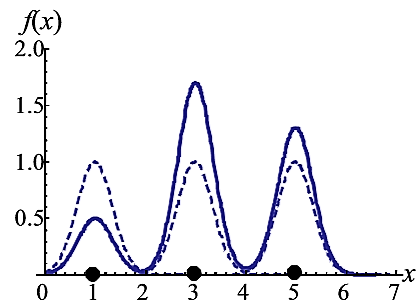
\includegraphics[width=1\linewidth]{figures/GaussianWidthSmall.png}
		\caption{Small Value \label{FigSmallWidth}}
	\end{subfigure}%
	\begin{subfigure}{.5\textwidth}
		\centering
		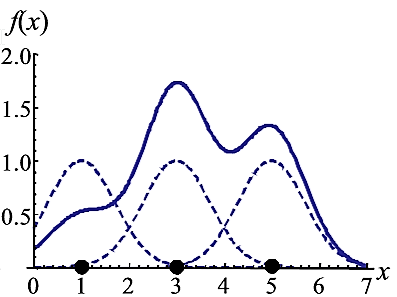
\includegraphics[width=1\linewidth]{figures/GaussianWidthLarge.png}
		\caption{Large Value \label{FigLargeWidth}}
	\end{subfigure}
	\caption[Effect of width in Gaussian Kernel for Regression]{The Effect of regression concerning the width of the Gaussian kernel.\cite{Kitayama.2011}}
	\label{FigGaussianWidthRegression}
\end{figure}
\FloatBarrier
To calculate the distance in practice, we are using a dissimilarity matrix $\mathbf{D}_{K,K}$.
This matrix employs the Euclidean distance with $d_{i,j}=||x_i-x_j||^2, \forall i,j \in \mathbf{D}$ as dissimilarity measure.
This matrix is symmetric and is zero on the diagonal.\cite[p. 22,299]{Gentle.2007}\newline
Because the Gaussian kernel is used in this approach, the dissimilarity matrix is already involved in the computational complexity.
Therefore, this matrix has just to be calculated once and can be reused in the theta estimation and the Gaussian kernel.
Another important thing to notice is that the data is already z-scored in the preparation and therefore there is no need to do it twice.
With this, we just search the maximum distance with the built-in MatLab function \textit{min()} and can proceed with \eqref{EqMaxDist} in Step 3.
In the tests, we are using the whole dataset including training and testing.\\
Although we can reduce the complexity with a clever implementation, the complexity discussion is based on the worst case involving all steps to compute.
The computational complexity of calculating the dissimilarly matrix is $\mathcal{O}(K^2)$.\cite{Kobti.2007}
Furthermore, finding a maximum in $K$ rows with $D$ values can be solved in $\mathcal{O}(KD)$.
Because the dissimilarity matrix is symmetric the complexity changes to $\mathcal{O}(N^2)$ and multiplying a scalar to $K$ elements costs $\mathcal{O}(K)$, which can be summarized in $\mathcal{O}(K^2+K)=\mathcal{O}K^2)$.
Again finding a minimum within the theta array from step four takes $\mathcal{O}(K)$.
Summarizing, we can obtain the complexity of the theta estimation with $\mathcal{O}(K^2)$.
Note that in practice, we have no insight into the built-in MatLab function, which algorithm or implementation is used.
Because of this, the performance may be better for finding a minimum.
Furthermore, we observed for small datasets, that the theta would be large, which will eventually lead to a worse performance, see section \ref{EmSecDaDes} and table \ref{TableThetaEst}.
\subsection{Training Algorithm}\label{InSubSecTraining}
With the results from the previous section, \acs{PCTKVM} is presented in algorithm \ref{PseudoCodePCTKVM}.
\begin{algorithm}
	\caption{Probabilistic Classification Transfer Kernel Vector Machine (Short)}\label{PseudoCodePCTKVM}	
	\begin{algorithmic}[1]
		\Require Input Data $\mathbf{K} = [\mathbf{Z};\mathbf{X}]$ as $N$ sized training and $M$ sized text set; $\mathbf{Y}$ as $N$ sized training label vector; kernel(-type) \textit{ker}; eigenspectrum dumping factor $\zeta$; $\theta$ as kernel parameter; \textit{niter} as maximal number of iterations; \textit{threshold} $\tau$ as convergence criteria; \textbf{InitVector} as $N$-sized initialization vector.
		\Ensure Weight Vector $\mathbf{w}$; bias $b$, kernel parameter $\theta$; transfer kernel $\expP{\mathbf{K}}_\mathcal{A}$.
		\State $\mathbf{D}$ = calculate\_Dissimilarity\_Matrix($\mathbf{K}$);
		\State $\theta$ = theta\_Estimation($\mathbf{D}$);  \Comment{According to section \eqref{InSubSecTheta} (optional)}
		\State $\expP{\mathbf{K}}_\mathcal{A}$ = transfer\_Kernel\_Learning($\mathbf{D}$,\textit{ker},$\theta$,$\zeta$); \Comment{According to \eqref{InSecTrans}}
		\State [$\mathbf{w}$,$b$] = pcvm\_Training($\expP{\mathbf{K}}_\mathcal{Z}$,\textbf{InitVector},\textit{niter},$\tau$); \Comment{Algorithm \eqref{PseudoCodePcvm}}
	\end{algorithmic}
\end{algorithm}
Note that the complete algorithm which involves every detail is found in appendix \ref{appac}. As already discussed, we are reusing the dissimilarity matrix. Therefore, the function parameters of \textit{transfer\_kernel\_Learning($\mathbf{D},\cdot$)} from algorithm \ref{PseudoCodeTKL} changing from using the raw data to using the dissimilarity matrix.  
We observed in practice that the kernel is for some $\theta$, not \acs{PSD} anymore, although he is in theory.\cite{Long.2015}
We assume that there is some issue in the floating point multiplication for small numbers in MatLab and therefore added the regularization term $eps\mathbf{I}_{K\times K}$ to the kernel, which solved the problem.\\
As it can be seen the \acs{PCTKVM} the number of free parameters remains the same because the $\theta$ is estimated, only the eigenspectrum dumping factor $\zeta$ is left.
Furthermore, we obtain by, combining the complexity of the theta estimation with the complexities of \acs{PCVM} and \acs{TKL}, the same complexity as already discussed, which is $\mathcal{O}(N^3+M^2)$.
This is achieved by reusing the dissimilarity matrix for the parameter estimation and the kernel function.
This statement can be validated in practice with table \ref{TableMeanTimeRank}, which shows that the \acs{PCTKVM} version with fixed theta and the algorithm with estimation need a similar time.
\subsection{Prediction}\label{InSubSecPrediction}
Additionally, we can make predictions based on the provided prediction function of the \acs{PCVM} with the use of $\expP{\mathbf{K}}_\mathcal{XZ} = \mathbf{U}_\mathcal{X}\mathbf{\Lambda}\expP{\mathbf{U}}_\mathcal{Z}^T$ as the kernel.
When it comes to the \acs{SVM}, the kernel has size $N\times M$ is used for the prediction according to the support vectors.
The prediction function for the \acs{SVM} from section \ref{PcSecSVM} has the form $\mathbf{y} = \expP{\mathbf{K}}_\mathcal{XZ}(\mathbf{\alpha}\odot\mathbf{y}_\mathbf{Z})+b$, where $\mathbf{\alpha}$ are the Lagrange multipliers.\cite{Long.2015}\newline
However, because of the sparsity of the \acs{PCVM}, the kernel size is greatly reduced as discussed in section \ref{Pc}.
If we consider that our model has $B$ non-zero weight vectors with $B\ll N$ and because the \acs{PCVM} uses only kernel rows/columns corresponding to the non-zero weight vector index, then our final kernel $\expP{\mathbf{K}}_\mathcal{KX}$ for prediction has size $(B\times M)$.
Therefore the prediction function of the \acs{PCTKVM} has the form:
\begin{equation}
\mathbf{y} = \expP{\mathbf{K}}_\mathcal{KX}\mathbf{w}+b
\end{equation}
Finally, the class label is obtained from the sign of the elements $y_i$ of the test label vector $\mathbf{y}_\mathcal{X}$ which has size $M$.
The probabilistic output is calculated with the probit link function as the \acs{PCVM} does it in equation \ref{EqPcGausLike}.

\subsection{Extensions}\label{InSubSecExt}
In the course of this work, because the Image dataset has more than two classes, there was the need to implement a multi-class option for the \acs{PCVM}, \acs{PCTKVM} and \acs{PCTKVM}\textsubscript{$\theta$Est}.\\
In general, there are many approaches to solve a multi-class problem for vector machines.\cite[p. 113]{Abe.2010}
According to the LibSVM documentation\footnote{\url{http://www.csie.ntu.edu.tw/~cjlin/libsvm/faq.html\#f419}}, for the LibSVM Library, two approaches are considered: The one vs. all and the one vs. one approach.
In the following, we will discuss the advantages and disadvantages for these two ideas and explain how it is integrated into the \acs{PCVM}.\\
The first is the one vs. rest approach.
Note that in the literature, the term one vs. all appears instead of one vs. rest.
If we consider $C$ classes, then the classifier would be trained with one class against the $C-1$ remaining classes.
This approach will have $C$ iteration, and in every iteration, another class is trained against each class.
The label assignment for one class is done in one iteration only.
However, this will lead to large unclassifiable regions in the feature space.\cite[p. 114-116]{Abe.2010}\newline
Therefore the second approach, one vs. one is implemented.
With this, we split up the labels in the different classes and train the classifier with every class against the others.
Again, if we take $C$, different classes, then our number of iteration is $I=C(C-1)/2$.
Furthermore, the unclassifiable region in comparison with the one vs. rest approach is smaller.
For the prediction, we do $I$ iterations again and predict the whole dataset with two classes.\cite[p. 127-128]{Abe.2010}\newline
In the implementation consider a test set with size $M$.
Then our label matrix $\mathbf{Y}$ and the probabilistic output matrix $\mathbf{P}$ has size $M\times K$.\\
We choose then the final label for the returning label vector $\mathbf{y}$ by counting the number of occurrences of a label for a data point.
The data point is then assigned to the label which the classifier has assigned the most.
In case of a tie the smaller class label, in terms of whole numbers, is assigned, according to the MatLab \textit{mode}\footnote{\url{https://de.mathworks.com/help/matlab/ref/mode.html}} function.
This is rather unconventional because it is likely to be a random selection, but in our tests, the results are the better as to assign the class label according to the biggest probability given from $\mathbf{P}$.\\
To determine a final probability output for a final label decision with concerning a data point, the algorithm calculates the mean of the probabilistic output for the runs where the label is equal to the final label is assigned.\\
The number of relevance vectors is determined by counting all unique vectors, which are used during the $K$ iterations.

\section{Conclusion}\label{InSecCon}
In this chapter, we successfully integrated transfer learning in the \acs{PCVM}.
We successfully integrated a proposed transfer learning method in the \acs{PCVM}, which forms the \acs{PCTKVM}.
Furthermore, we solved the problem that the algorithm will be slow through the theta optimization by adopting a simple theta estimation and adjust it to the needs of the \acs{PCVM}.
Because it uses unlabeled target data, the algorithm is transductive and solves the transfer problem with a relational-knowledge approach regarding homogeneous transfer learning.\\
Additionally, we extend the \acs{PCVM} and \acs{PCTKVM} to being able to solve multi-class problems via the one vs. one approach.
The MatLab source code of the \acs{PCTKVM} and \acs{PCTKVM}\textsubscript{$\theta$Est} can be obtained from Github\footnote{\url{https://github.com/ChristophRaab/pctkvm.git}}.
Furthermore, the reader can find the complete code written for this thesis, including all tests, in the repository.

\chapter{Benchmark Study}\label{EmChap}
In this chapter, the preparations and the result of the study are described.
With this, the used datasets to determine the performance are defined, and the set of transfer learning classifiers with the corresponding parameters are appointed.\\
Furthermore, the used statistical methods in the study are introduced, and the statistics are shown and discussed.
This study is split up in three parts of statistics.
The first part is a basic descriptive statistics to give an overview of the general performance of the classifiers.
This is followed by the comparison of classifiers over one dataset and finally over multiple datasets.
With that, all datasets described in this thesis are tested.\\
The procedure and selection of statistics are mainly adopted from \cite{Chen.2009} and \cite{Long.2015}.
The main reason for this is to guarantee a fair comparison of the \acs{PCVM}, \acs{PCTKVM} and the \acs{TKL} method as wrapper algorithm for the \acs{SVM}.\\
On first sight, it may be strange to compare first the difference between single datasets and proceed with an overall test.
This is made because of two analytic reasons. First, the study has two different kinds of datasets (image and text) and many subcategories and subsets.
With the single test, it can be determined if there is a significant difference between the performance of classifiers and datasets.
When it comes to a real-world scenario, the choice of a classifier may depend on his strengths and weaknesses to solve a task on a specific kind of dataset.
With this listing of the performance may one can choose more precisely which classifier he chooses for the job. At least for text documents and images.\\
On the other hand from the scientific point of view, the comparison over all used datasets and the results in performance giving the most useful insights.\\
Note that in this chapter for clarity only the aggregated results are shown. The complete results are shown in appendix \ref{appaB}.

\section{Dataset Description}\label{EmSecDaDes}
The study consists of 18 benchmark datasets.
Three of them are text-based from Reuters-21578\footnote{\url{http://www.daviddlewis.com/resources/testcollections/reuters21578}} and the remaining twelve are images from Caltech-256\footnote{\url{http://www.vision.caltech.edu/Image\_Datasets/Caltech256/}} and Office.
Note that the datasets are not extracted from the raw data, but rather used from others with a pre-processing state.
The corresponding articles, which are use this version of datasets are \cite{Gong.} and \cite{Long.2015}.
\\
This 18 sets are well known in the area of domain adaptation and transfer learning and for example used in 
\cite{Long.2015}\cite{Gong.}\cite{Fernando.}\cite{Long.}\cite{Dai.}\cite{Quattoni.} and discussed in \cite{Pan.2010}.\\
A crucial characteristic of the datasets is that the domains for training and testing are different but related.
This relation exists because the train and test classes have the same top category or source.
The classes themselves are subcategories or subsets.\cite{JingGao.2008}\\
The relation will be clear in the separate sections for the datasets respectively.

\subsection{Text Dataset}\label{EmSubSecText}
The Reuters-21578 collection appeared on the Reuters news-wire in 1987.
The documents were assembled with categories by personnel from Reuters Ltd. and \ac{CGI}.
Reuters and \acs{CGI} published the documents for research purposes.\cite{DavidD.Lewis.2004}\\
It is a frequently used text collection to evaluate the performance of text categorization techniques.
The collection is segmented in five top categories and many subcategories.
For testing classifiers, the task is to evaluate on three big categories \textit{orgs}, \textit{people} and \textit{places}. 
In the last subcategory, all documents about the USA are removed.
This makes the categories nearly even because more than a half of the documents are in the USA subcategory. 
Furthermore, some pre-processing is done at the collection.\cite{WenyuanDai.2007}\\
First, all letters are converted to lower case, and the words are stemmed using the Porter stemmer.
This stemmer removes the suffixes form the terms.\cite{Porter.1997} 
Furthermore, stopwords are removed. With the \ac{DF} Threshold, the numbers of features are cut down.
To apply the \acs{DF} Threshold the number of documents in which a certain term occurs has to be count.
Each term which is less than a previously set threshold is removed from the feature space.\cite{Yang.1997}
The Threshold parameter is set to three with the goal to speed up the classification process.
Finally, \ac{TFIDF} is applied for feature generation.
The \acs{TFIDF} value is used to train the classifiers.
The \acs{TFIDF} is a measure of how well a term characterizes a document.
It takes the frequency of a term in a document times the inverse document frequency which is the number of occurrences of this term in all documents. \cite[p. 26]{Leskovec.2014}\\
For the domain adaptation purpose, six datasets were generated from Reuters-21578:
\textit{orgs vs. places}, \textit{orgs vs. people}, \textit{people vs. places}, \textit{places vs. orgs}, \textit{people vs. places} and \textit{places vs. people}.
The labels are created by assigning orgs for example as positive class and people as the negative class.
Furthermore, the two labels are split by its subcategories to create the training and test sets.\cite{WenyuanDai.2007}\\
In table \ref{TableSumReuters} the dataset with its features, observations, labels and the corresponding divergences, \acs{KLD} and \ac{MMD}, are shown.
The divergences are defined in Section \ref{TlSubSecKLD}. \\
To get an overview of the distribution and its transfer learning purpose the \textit{orgs vs. people} dataset is shown in Figure \ref{FigOrgVsPeoplePlot}.
\begin{table}[]
	\centering
	\resizebox{\textwidth}{!}{%
	\begin{tabular}{c|cccc|c|c}
		Top Category     & \#Examples 1 & \#Examples 2 & \#Features       & \# Labels      & \ac{KLD} & \ac{MMD}\\ \hline
		Orgs vs. People   & 1237                  & 1208                  & \multirow{3}{*}{4771} &	\multirow{3}{*}{2} & 0.4570  &   0.0410  \\
		Orgs vs. Places   & 1208                  & 1016                  &                       &	 					& 0.7420  &  	0.0455 \\
		People vs. Places & 1016                  & 1208                  &                       &						 &  0.6690 &	0.0421   
	\end{tabular}}
	\caption[Overview of key values of Reuters-21578 dataset]{Overview of the key figures of the Reuters-21578 dataset	\label{TableSumReuters}}
\end{table}


\begin{figure}
	\centering
	\begin{subfigure}{.5\textwidth}
		\centering
		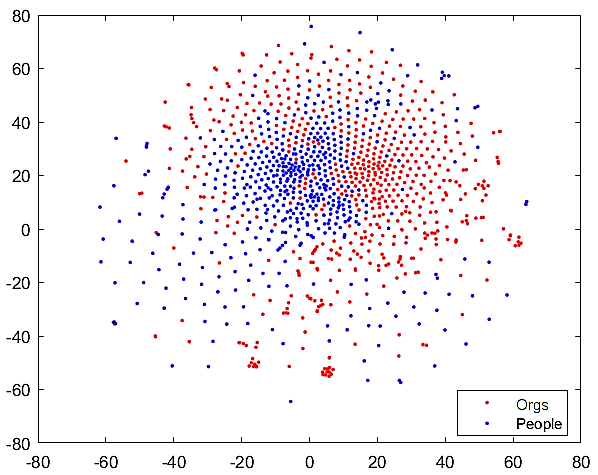
\includegraphics[width=1\linewidth]{figures/Plot_Train_OP_1.png}
		\caption{Training Set\label{FigOPSub1}}
	\end{subfigure}%
	\begin{subfigure}{.5\textwidth}
		\centering
		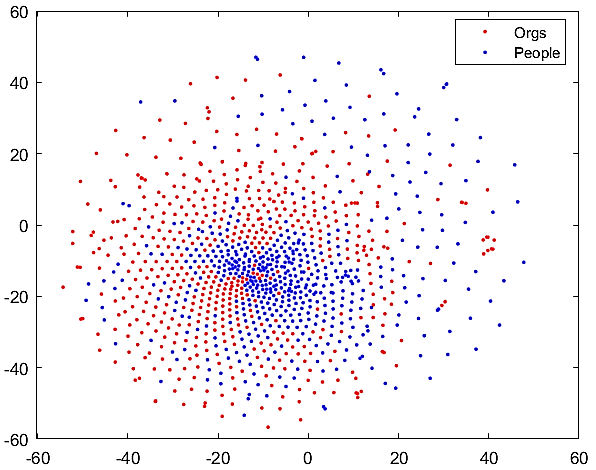
\includegraphics[width=1\linewidth]{figures/Plot_Test_OP_1.png}
		\caption{Test Set\label{FigOPSub2}}
	\end{subfigure}
	\caption[Plot of Orgs vs. People Dataset]{The plot of the \textit{Orgs vs. People} dataset. One the left hand is the training set, and on the right, the test set is shown. The dimension is reduced with t-SNE to two dimensions. The \acs{KLD} to the original Dataset is 2.233 and 2.464 	\label{FigOrgVsPeoplePlot}}
\end{figure}

\subsection{Image Dataset}\label{EmSubSecIm}
\begin{table}[]
	\centering
	\resizebox{\textwidth}{!}{%
		\begin{tabular}{c|cccc|c|c} 		Name    			& \#Examples 1			& \#Examples 2 	 	   & \#Features       	   & \# Labels      		& \ac{KLD} & \ac{MMD}\\ \hline
			Caltech vs. Amazon  	& \multirow{3}{*}{1123} & 958                  & \multirow{3}{*}{800} &	\multirow{3}{*}{10} & 1.2062   & 0.0449  \\
			Caltech	vs. DSLR 	&                	 	& 295                  &                      &	 					& 1.1418   & 0.0654 \\
			Caltech vs. Webcam 	&                  		& 157                  &                      &						& 1.1567   & 0.0852 	
	\end{tabular}}
	\caption[Overview of key values of Image dataset]{Overview of the key figures of the Image dataset}
	\label{TableSumImage}
\end{table}
The image dataset has two main Parts. 
The first one which is named \textit{office} in this thesis and is collected and created from \cite{Saenko.2010}.
This contains various images from three different sources which are forming the four datasets.
One are images taken from the web downloaded from the online merchant's \textit{amazon} (Name in Dataset).
Originally 31 categories, which are different types of products, with an average of 90 images are captured.
The objects are typically shown from a canonical viewpoint.\\
A canonical viewpoint is a certain view of an object in a certain rotation, which is considered as 'good' to recognize the object correctly. \cite{Edelman.1991}\\
The second consists of images that are captured with a digital SLR camera (\textit{dslr}).
The conditions should be realistic environments (\textit{office}) and natural lighting.
The resolution of the images is high with low noise.
With that 31 object categories within five different objects are taken.
An object contains on average three images, taken from various viewpoints.
This makes a total of 423 images.\cite{Saenko.2010}\\
The image dataset has two main Parts. 
The first one which is named \textit{office} in this thesis and is collected and created from \cite{Saenko.2010}.
This contains various images from three different sources which are the different datasets respectively.
One are images taken from the web, downloaded from the online merchants \textit{amazon} (Name in Dataset).
It has originally 31 categories, which are different types of products, with an average of 90 images are captured.
The objects are typically shown from a canonical viewpoint.\cite{Saenko.2010}\\
The last set of images are from a \textit{webcam}.
Images are taken from this, with a low resolution with a high noise. The purpose of this is to simulate sensors that are similar to robotic sensors.
It has the same 31 categories with five objects per category and a total of 795 images. \\
The second main part of this dataset is from \cite{GregGriffin.} and is called \textit{Caltech-256}. In comparison with the other image collections, the \textit{Caltech-256} dataset is much larger.
It has an average of 119 images per category in 257 categories with a total of 30607 images.
They are crawled from Google and PicSearch but duplicates are deleted.\cite{GregGriffin.}\\
The \ac{SIFT} approach transforms images into scale-invariant coordinates relative to local features which are 'summarized' in key point descriptors.\cite{Lowe.2004}
With this images with over 15 similar \acs{SIFT} descriptors are removed.
The images are sorted in a category itself by the amount of how good this one represents the category.
The Range goes from "Good: A clear example of the visual category" to "Not Applicable: Not an example of the object category.\cite[p.3]{GregGriffin.}\\
To get an overall collection of the four image sets which are considered as domains, categories with the same description are taken.
From the 31 and 256 categories ten similar categories are extracted:
backpack, touring-bike, calculator, head-phones, computer-keyboard, laptop-101, computer-monitor, computer-mouse, coffee-mug and video-projector.
They are the class labels from one to ten. 
With this, a classifier should be trained on the training domain and should be able to classify the test image to the corresponding image category.
The final feature extraction is done with \ac{SURF} and encoded with 800-bin histograms.
Finally, the twelve sets are designed to be trained and tested against each other by the ten labels.\cite{Gong.} \\
The \ac{SURF} Algorithm uses integral images for images convolutions and uses existing detectors and descriptors and reduced the used methods to the essentials. \cite{vanBay.2006} 
In figure \ref{FigExampleImages} there are some example images taken from the four datasets of the category computer monitor. 
As in \ref{EmSubSecText}, some key figures from the dataset are pointed out in table \ref{TableSumImage}.
Note that for clarity, not the twelve datasets are shown, but rather only the 'caltech vs. others'.
The remaining sets should be similar.
\begin{figure}[]
	\centering
	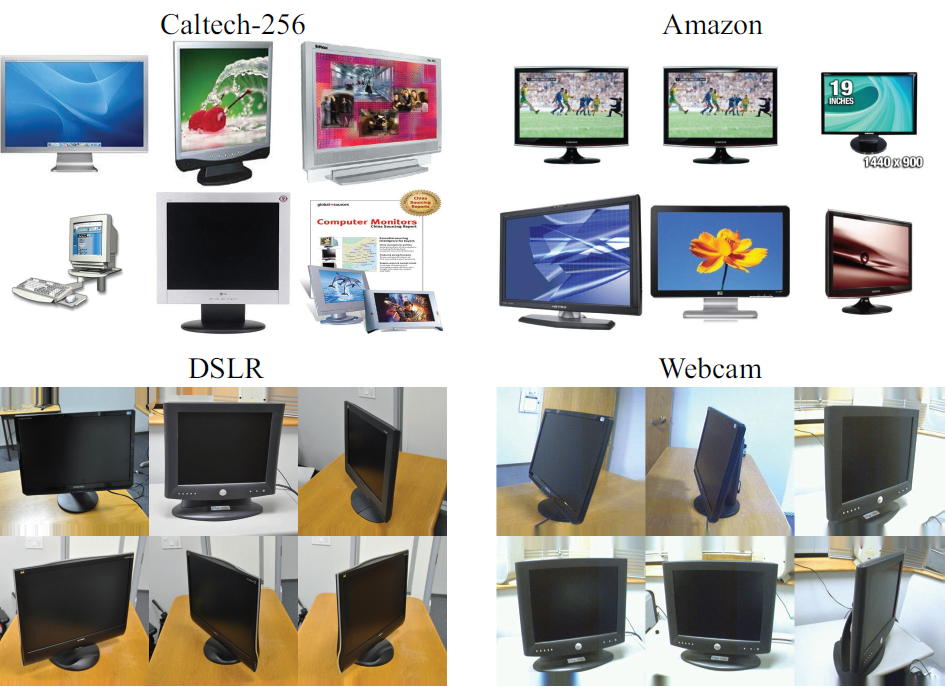
\includegraphics[width=.8\linewidth]{figures/ExampleImages.png}
	\caption[Example from Image Dataset]{Examples Images from the four Image Datasets Caltech10, Amazon, DSLR, Webcam. \cite{Gong.}}
	\label{FigExampleImages}
\end{figure}
\section{Study Procedure and Settings}\label{EmSecStudy}
In this part, the data sampling, parameters and the used kernels are introduced.
Every transfer learning method, which is used in the study is already introduced in chapter \ref{Tl}.
Note that for a fair comparison the heterogeneous methods are not included in the study because they solve a different problem from the \acs{PCTKVM}, which is described above in section \ref{TlSecHetero}.
The basic task in this study is classification with data from the same feature space.\\
The \ac{SVM} and the \acl{PCVM} are the baseline classifier in this study.
The \acs{PCVM} is described in section\ref{Pc}.\\

\subsection{Data Sampling}\label{EmSubSecDataS}
The samples for testing the classifiers are drawn with five times two-fold cross-validation manner.
However, to obtain the differences from training- to test-set and the resulting transfer learning attributes, a sample is not drawn from the dataset as one, but rather obtaining the different domains and draw from one only for training or testing.
This means for example, the two image sets \textit{amazon} and \textit{webcam} are not merged.
Furthermore, the comparability of this study with another study would be lost.
The training set is sampled from \textit{amazon} and the test is from \textit{webcam}.
This is a suggested standard method for cross-validation in transfer learning.\cite{Gong.}
Furthermore, the datasets are normalized via z-scored.
This can be obtained from equation \ref{EqZTrans} in section \ref{InSubSecTheta}.
\subsection{Kernel}\label{EmSubSecKernel}
A kernel in this work is a symmetric matrix, in the following $\mathbf{K}$, which has to be positive semi-definite and therefore satisfies the Mercer conditions and integrates a similarity (dissimilarity) measure.
It is an inner product of $N$ training patterns, represented as vectors, which is a $N \times N$ matrix:
\begin{equation}
	\mathbf{K}(\mathbf{x},\mathbf{x'}) = \phi(\mathbf{x})^T\phi(\mathbf{x'})
\end{equation}
With $\phi(\cdot)$ as explicit feature mapping function.
Because of its symmetry $\mathbf{K}(\mathbf{x},\mathbf{x'})=\mathbf{K}(\mathbf{x'},\mathbf{x})$.
In its simplest form, the linear kernel, the function becomes $\phi(\mathbf{x}) = \mathbf{x}$ which results in the simple vector dot product $\mathbf{x}\mathbf{x}^T$ as similarity measure. There are various kernels and techniques to construct it. For example, if one replaces the inner product with some metric, e.\,g., Euclidean distance, then the kernel functions are referred as basis- instead of feature mapping functions.\cite[p. 291-296, 329]{Bishop.2009}\\
In this study almost all kernel machines are using a modified version of the \ac{RBF}- or Gaussian-Kernel.
The 'well known' kernel can be obtained from \cite[p. 17]{Vert.2004} and has the form:
\begin{equation}\label{EqRBFOriginalKernel}
	k(\mathbf{x},\mathbf{x}') = \exp\frac{d(\mathbf{x},\mathbf{x}')^2}{2\sigma^2}
\end{equation}
Where $d$ is the Euclidean distance and sigma is the width of the Gaussian kernel.\\
The used one is suggested from \cite{Duan.2012} and 'replaces' the $\sigma$ parameter with $\frac{1}{A}$ and $A$ as median over the samples: 
\begin{equation}\label{EqRBFAKernel}
	k(\mathbf{x},\mathbf{x'}) = \exp(-\frac{1}{A}\abs{\mathbf{x}-\mathbf{x'}}^2)
\end{equation} 
Note $\gamma = \frac{1}{A}$ is a used abbreviation in \cite{Long.2015}.
There are two classifiers with different kernels.
First, the \acs{GFK} uses the implementation of an own supervised $k$ nearest neighbor approach which can be obtained from the website of the author \ref{TlSubSecHomoSymFeature}.
Second, the \acs{PCVM}, because in the cross-validation state for determining the parameters, the performance drops dramatically with the use of \eqref{EqRBFAKernel}.
Therefore the \acs{PCVM} uses the proposed \acs{RBF}-Kernel from \cite{Chen.2009}. 
\begin{equation}\label{RBFKernelPCVM}
k(\mathbf{x},\mathbf{x'}) = \exp(-\frac{\abs{\mathbf{x}-\mathbf{x'}}^2}{\sigma^2})
\end{equation}
The rest is trained with the suggested one from \eqref{EqRBFAKernel}, although they are used to train with \eqref{EqRBFAKernel}, which is obtained by the source code from the methods.
However, the \acs{TKL} approaches are using it initially.
This is done to compare the pure transfer performance, as independent as possible.

\subsection{Parameters}
The cost Parameter $C$ of the \acs{SVM}, which controls the trade-off between margin and the ability to adapt the decision boundary to points near to it, is set to 10. \cite[p. 421-422]{TrevorHastie.2009}
Finally, the LibSVM implementation which can work with pre-calculated kernels is used. The kernel is described above in section\ref{EmSubSecKernel}.\\
The PCVM as baseline Classifiers has only one parameter $\theta$, which is set to 1 for both sets.
Furthermore, \textit{niter} is set to 600 because we observed that the \acs{PCVM} often terminates somewhere between 500-600 iterations. The threshold is set to 0.001.\\
The parameters for the transfer learning methods are partly obtained from the corresponding papers or with cross-validation. 
The \acs{PCTKVM} and \acs{TKL} algorithms are mainly using the eigenvalue dumping factor $\xi$ which is set to two for the text datasets and 1.1 for the image datasets.\cite{Long.2015}
Furthermore, the \acs{PCTKVM} uses the new kernel with $\gamma=\frac{\sigma}{A}$ in \eqref{EqRBFAKernel}.
Because of that, there is another parameter $\sigma$ which is set to two for the text sets and one for the image datasets.
When it comes to the sigma estimation for \acs{PCTKVM}\textsubscript{$\theta$Est} described in section \ref{InSubSecTheta} the $\sigma$ value is determined for every dataset respectively.
The estimated sigmas are summarized in table \ref{TableThetaEst}. \\
\acs{JDA} has two Model parameters.
First the number of subspace bases $k$, which is set to 100 and the regularization parameter $\lambda $ which is set to one for both.\cite{Long.}\\
For the \acs{GFK} solution the parameter, number of subspace dimensions are evaluated with cross-validation from $k=\{1,5,10,20,...,100,200\}$ and finally set for the text sets to 40 and to 50 for the image sets.\\
The \acs{TCA} has also one parameter which gives the subspace dimensions and are determined from $\mu=\{1,5,10,20,...,100,200\}$ and is set to $\mu=50$ for both datasets.\\
The goal of the parameter determination procedure was to identify the best performance concerning the parameters.
\begin{table}[]
	\centering
		\begin{tabular}{|c|c||c|c|}
			\hline
			Dataset         & Theta & Dataset & Theta \\ \hline
			Org vs. People   & 1.415 & C vs. D  & 2.187 \\ \hline
			Org vs. Place    & 2.224 & A vs. W  & 2.152\\ \hline
			People vs. Place & 2.187 & A vs. D  & 2.166\\ \hline
			C vs. A          & 2.224 & D vs. W  & 2.163 \\ \hline
			C vs. W          & 2.187\\ \cline{1-2}
	\end{tabular}
	\caption[List of estimated Thetas]{List of the estimated Thetas based on text and image datasets.\label{TableThetaEst}}
\end{table}

\section{Performance Metrics}\label{EmSubSecPerMet}
The Performance of the transfer learning classifier has to be determined and should be compared with others.
There are several metrics which can be used to measure the performance of a classifier.\\
However, before these are defined, there are some basic definitions to make, which are applied to the metrics in the following sections.
These definitions are helping to get an idea of the location- and distribution characteristics of the sample.\cite[p. 216-217]{Teschl.2014}
First, the mean which gives the average value of samples. 
\begin{equation}\label{EqMean}
	\mean{x} = \frac{1}{N}\sum_{i=1}^{N}x_i
\end{equation}
This samples can be for example one of the key figures of one classifier for the 18 datasets. 
The standard deviation is formulated to measure how the samples are distributed around the mean.
\begin{equation}\label{EqStandardDeviation}
s^2=\sqrt{\frac{1}{N-1}\sum_{i=1}^{N}(x_i-\mean{x})}
\end{equation}
In both \eqref{EqMean} and \eqref{EqStandardDeviation}, $N$ is the number of samples. \\
The null hypothesis in this context has the assumption that two classifiers are equal.
If not this hypothesis is rejected.\cite{Alpaydm.1999} 
To determine if the null hypothesis can be rejected, is the goal of the statistics from \ref{EmSubSecResOneDa} and \ref{EmSubSecResMulDa}.
However, before this decision can be made, the performance of an algorithm has to be captured.
In this thesis four key figures are used.
For clarity, the key figures are represented in the result table in percent.
This differs from the origin calculation presented here.
The selection of the key figures is influenced by \cite{Chen.2009}.\\
\subsection{Area under a ROC Curve}
The first metric is the \ac{AUC} which measures exactly what the name says.\cite[p. 13]{Fawcett.}\\
A \ac{ROC} Curve is a technique for visualizing and organizing classifiers based on their performance.
This curve sometimes also called graph is a two-dimensional plot of the true positive rate on the Y axis and the false positive rate on the X-axis.
It illustrates the trade-off between the benefits and costs.
The more the graph heads north-west, the better is the classifier.
Note that if a classifier has a low \ac{ROC} curve near the X axis, then it may be conservative in making an assignment to a positive class because it makes it only with strong evidence.
That means it makes few false positive errors, but they often have a low true positive rate.\cite[p. 4]{Fawcett.}\\
In this thesis, when it comes to two classes, it is interpreted as a lower performance, because the true positive points have a higher probability to be wrongly classified concerning the
negative label.\\
Because the \ac{AUC} is an area in a unit square, it has a value between zero and one.
The statistical interpretation is as follows: "The \acs{AUC} of a classifier is equivalent to the probability that the classifier will rank a randomly chosen positive instance higher than a randomly chosen negative instance."\cite[p. 13-16]{Fawcett.} \\
Concerning a two-class problem, the \acs{AUC} tells us the probability for a member of the positive class and the negative class that the positive one is correctly classified to the positive class and the other respectively. 
For this thesis the built-in MatLab function \textit{[X,Y,~,AUC] = perfcurve(LABELS,SCORES,POSCLASS)} is used.
The function needs the ground truth 'LABELS' and the probabilistic estimate that this point actual belongs to the positive class ('SCORES') determined by a classifier.
With 'POSCLASS' the positive class is specified. In this thesis, '1' is always the positive class.
It gives the arrays X and Y back to create the ROC curve as MatLab plot.
The function output 'AUC' is the needed value for comparison.
Note that with this definition of \acs{AUC}, it makes only sense for two class problems.
For the multi-class problems, the accuracy is more insightful, but the \acs{AUC} is calculated for completeness with '1' as positive label and the rest of the labels as negative.\\
\subsection{Accuracy and Error}
The accuracy is another used metric with:\cite{Long.2015}
\begin{equation}
	Accuracy = \frac{| x : x \in \mathcal{X} \wedge f(x) = y(x)|}{|x : x \in \mathcal{X}|}
\end{equation}
With $f(x)$ as the given label from the classifier and $y(x)$ as the ground truth label.
In other words, it describes how many of the test points are getting the correct labels from a classifier assigned concerning all points.\\
Another way to interpret the accuracy is that it is the relation of the true positive rate and true negative rate to all samples.
The accuracy goes from zero to one because it is normalized.\cite[p. 3]{Fawcett.}
In this thesis, the metric \ac{ERR} is simply calculated with  $Error = 1 - Accuracy$.\\
\subsection{Root Mean Squared Error}
The last metric is the \ac{RMSE}. It takes the root of the squared mean errors.
\begin{equation}
	RMSE = \sqrt{\frac{1}{N} \sum_{i=1}^{n}e_i^2}
\end{equation}
With $N$ as the number of errors which relies on the number of datasets. The \ac{RMSE} assumes that the errors are normal distributed and unbiased.
It is per definition always higher than the simply \ac{MAE}.
With that, the \acs{RMSE} tends to become increasingly larger in comparison with the \acs{MAE}, as the distribution of the error magnitude becomes larger. 
The \acs{RMSE} penalizes the variance of errors by weighting larger absolute errors more than smaller ones.
Note that the \acs{RMSE} is sensitive to outliers.
This key figure is another idea trying to describe the error distribution. \cite{Chai.2014}
\FloatBarrier
\section{Descriptive Statistics}\label{EmSecTest}
In this section, the general performance of the classifiers is shown.
As part of the descriptive statistics, the mean and the standard deviation are used.\cite{Igual.2017}\\
With that, the different key figures over the datasets are summarized.
The performance, in general, is divided into datasets. The full result can be considered in appendix \ref{appaB}.

\subsection{Metric Results}\label{EmSubSecMetricResult}
\begin{figure}
	\centering
	\begin{subfigure}{.5\textwidth}
		\centering
		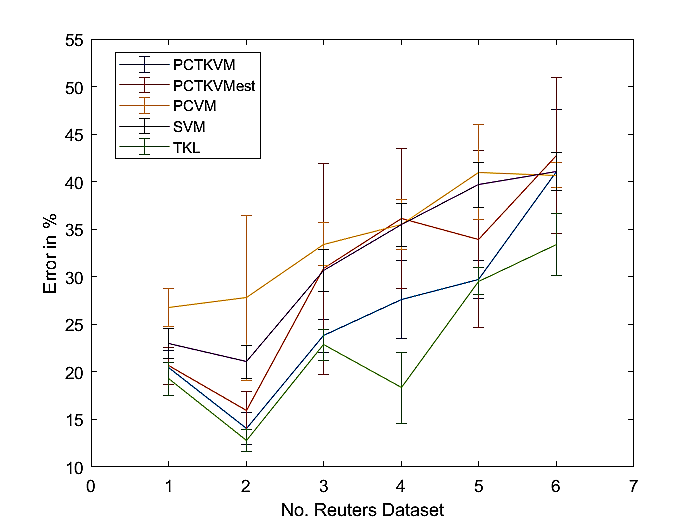
\includegraphics[width=1\linewidth]{figures/PerformanceReuters.png}
		\caption{\label{FigErrorReu}}
	\end{subfigure}%
	\begin{subfigure}{.5\textwidth}
		\centering
		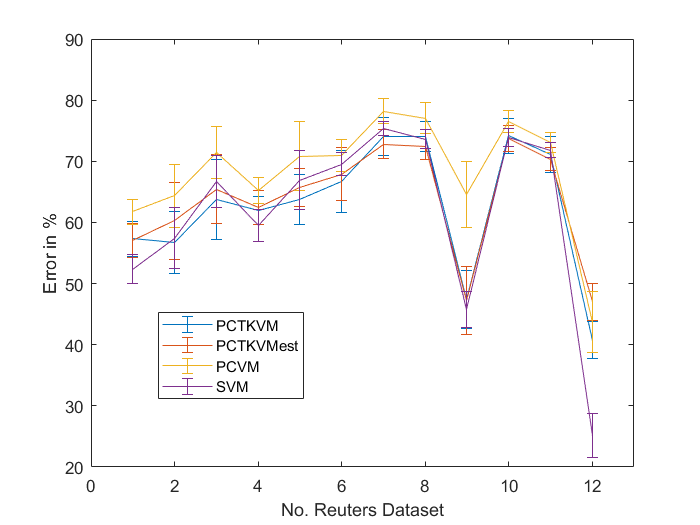
\includegraphics[width=1\linewidth]{figures/PerformanceImage.png}
		\caption{\label{FigErrorImg}}
	\end{subfigure}
	\caption[Plot of mean Error and standard Deviation]{The plot of mean errors with standard deviation of the cross-validation. The left shows the result on Reuters and the right shows the result on images. A graph shows the error and a vertical bar shows the standard deviation. \label{FigErrorDatasets}}
\end{figure}
In this subsection, the performance over the metrics, which are described earlier, is shown.
In general, according to the \acs{MMD}'s and \acs{KLD}'s for the 18 datasets, classification of an image datasets is a more challenging problem in comparison with the Reuters dataset.
The results are summarized in table \ref{TableDescriptiveStatistics}. 
Note that this data is produced on the fly in the 5x2 cv F test. Therefore the shown results are the mean over ten repetitions of cross-validation.
The standard deviation is shown in brackets. 
The results are split up in the two dataset categories Image and Reuters, respectively.
Furthermore, the four metrics error, \acs{RMSE} and \acs{AUC} are applied.
The \ac{ACC} can simply be determined with the error.
The classifiers, which are created in the course of this work in italics.
The performance of the best classifier is bold.
The \acs{GFK} implementation supports no probabilistic output and therefore has no \acs{AUC} value in general.
Note that through a cross-validation on the 18 datasets, the means metrics are combined from 180 performance results.
Furthermore, the mean error over Reuters and image datasets for the \acs{SVM}, \acs{TKL} and the \acs{PCVM}'s are shown in figure \ref{FigErrorDatasets}.
Note that the \acs{TKL} is excluded in the second image (\ref{FigErrorImg}) for clarity.
The error graph over the whole datasets and the remaining classifier are shown in \ref{appaB}.\\
It can be observed that the \acs{TKL} with the \acs{SVM} has the overall best performance. 
In general, and according to section \ref{TlSecNeg}, it can be seen that negative transfer happens between the baseline \acs{SVM} and the transfer solution \acs{GFK}.
However, we can see that the \acs{PCTKVM}  achieves an \textit{overall} better performance result than the \acs{PCVM} in this test.
Furthermore, the \acs{PCTKVM} can achieve better performance at text sets than the remaining transfer learning solutions and the \acs{SVM}.\\
The performance of the \acs{PCVM}'s at image datasets is comparable with the result of the \acs{SVM}, which is also observable in \ref{FigErrorImg}.
Nevertheless, this is also observable for the other transfer learning solutions, which are not very better as the \acs{SVM}.\\
We assume that this happens because the datasets are very small and the classes are not balanced because we can rather obtain a good performance on the larger more balanced text datasets in comparison with the \acs{SVM}.
This assumption may be more valid when one takes a look at the comparison, which involves the whole dataset, which is shown in table \ref{BTableCompleteErr}.
It seems that the \acs{SVM} can handle very small datasets better than the \acs{PCVM} in general.
However, again referring to the detailed test results, it states that the \acs{PCTKVM} is often the second best classifier.
The \acs{PCTKVM} does a better job as the other remaining transfer learning classifiers.\\
Additionally, we can see that the \acs{SVM} baseliner has an overall better performance than the \acs{PCVM} baseliner.
Apart from the size of datasets, it might be that because of the differences in the distribution caused by the dataset; it might be a better idea for transfer learning to find a hyperplane, which separates the classes best, rather than modeling it via probabilistic.
Therefore, and because \acs{SVM} is good at image sets, we assume that the \acs{SVM} boosts the performance of the transfer learning solutions more than the vice verse.\\
In fact, the performance is of the \acs{TKL} is always better than the performance of \acs{PCTKVM}.\\
Furthermore, we can observe that the \acs{PCTKVM}\textsubscript{$\theta$Est} is in general worse than the \acs{PCTKVM}. 
Because these two approaches only differ in the $\theta$ value, we can say that the $\theta$ estimation approach described in section \ref{InSubSecTheta}, doesn't works out very well.
In fact, the estimation was originally designed for regression and classification \cite{Kitayama.2011}. However, it seems that the value of the estimation is too 'smooth' and the probabilistic estimation for one class are 'overlapping' in the other classes space.
This space, would one intuitively assign to the other label.
This might be similar to the problem of the \acs{RVM} from \cite{Chen.2009}, Where it assigns a negative weight in the heart of the positive class.\\
The essence of the standard deviation in table \ref{TableDescriptiveStatistics} states the overall performance range in the datasets, which fluctuates concerning the composition of the datasets.
Therefore, to make a valid assumption on the standard deviation concerning the classifiers, we again have to look in the detailed result table \ref{BTableFTErr}.
As pointed out in the results of Chen et al. in \cite{Chen.2009} and with our results again, the range of standard deviation for the \acs{PCVM} is not that kind of a problem. 
However, when it comes to the \acs{PCTKVM}\textsubscript{$\theta$Est}, we see that the range of standard deviation, especially for the text datasets, is higher in comparison with the deviation of the remaining classifiers.
Since \acs{PCTKVM} and \acs{PCTKVM}\textsubscript{$\theta$Est} only differ in the theta value, we can say that the fluctuation of performance in this test also depends on the theta.
The fact that all \acs{PCVM}'s are randomly initialized is not critical because we can observe that the standard deviation is not greatly higher in comparison with the other classifiers form table \ref{BTableFTErr}. 
\begin{table}[]
	\centering
	\resizebox{\textwidth}{!}{%

	\begin{tabular}{@{}lccllcccc@{}}
		\toprule
		ERR     & SVM   & PCVM  & PCTKVM\textsubscript{$\theta$Est} & PCTKVM & TCA   & JDA   & GFK   & TKL              \\ \midrule
		Reuters & 31.82(2.02) & 34.19(3.65) & \textit{30.03}(6.63)    & \textit{26.12}(2.97)  & 30.87(3.24) & 32.95(2.54) & 34.53(2.74) & \textbf{22.70}(2.17) \\
		Image   & 61.51 (2.75)& 68.13(3.11) & \textit{63.53} (3.48)   & \textit{62.64} (3.35) & 59.56(3.33) & 59.39(3.32) & 64.24(2.96) & \textbf{58.25}(7.63) \\\midrule
		RMSE    & SVM   & PCVM  & PCTKVM\textsubscript{$\theta$Est} & PCTKVM & TCA   & JDA   & GFK   & TKL              \\
		Reuters & 31.88 (8.43) & 34.48(5.93) & \textit{30.77} (10.35)  & \textit{26.28} (9.32) & 31.03(9.00) & 33.05(8.81) & 34.63(6.28) & \textbf{22.81}(7.63) \\
		Image   & 61.59(14.71) & 68.23(6.88) & \textit{63.64} (9.15)   & \textit{62.76}(9.35)  & 59.67(14.76) & 59.50(14.81) & 64.33(15.39) & \textbf{58.36}(13.63) \\\midrule
		AUC     & SVM   & PCVM  & PCTKVM\textsubscript{$\theta$Est} & PCTKVM & TCA   & JDA   & GFK   & TKL              \\
		Reuters & 69.00 (2.33) & 70.96(3.99) & \textit{76.47} (8.63) & \textit{79.36}(4.82)  & 72.32(3.78) & 69.11 (3.13) & -     & \textbf{83.46} (2.26)\\ \bottomrule
	\end{tabular}}
	\caption[Result of Cross-Validation]{The results of the transfer learning classifiers with cross-validation under the four metrics on the 18 datasets.\label{TableDescriptiveStatistics}}
\end{table}
\FloatBarrier
\subsection{Time Results}\label{EmSubSecTimeResults}
The next comparison is over the mean computational time, which a classifier needed to train and test the datasets.
The baseline takes part in the time measure for the transfer learning solution because it is about to test for example if the \acs{SVM} can handle the subspaces or a different kernel in proper time.
Note that that the computational time is summarized in ranks.
The first rank is assigned for the fastest and the last for the slowest.
Average ranks are assigned for ties with respect to ranks.
With this, there are the means of the datasets combined, and the ranks are the result of it.
The table \ref{TableMeanTimeRank} shows the mean of these ranks.
The second row of the table shows the mean time over all 18 datasets in seconds.\\
The result of the time ranking is unambiguous, with the \acs{SVM} as the fastest classifier. 
However, this is no surprise, because it is beside the \acs{PCVM} the baseline classifier, and has because of this the lowest computational complexity, which results in lower training and testing time.
Obviously, because the other solutions are trying to do the transfer learning, which results in higher complexity.\\
Although the complexity of \acs{PCVM} and \acs{SVM} are comparable, in practice, more precisely, datasets with two domains, we observed that the $\theta$ optimization takes forever.
It seems that in the transfer learning setting, the local optimum for the next theta is hard to obtain.
Another point to mention is that the \acs{PCVM} does not converge very well and uses the full 500 iterations. 
This, combined with the $\theta$ optimization in every iteration, leads to the high computational time.\\
Although the ranks from \acs{PCTKVM}\textsubscript{$\theta$Est} and \acs{PCTKVM} are bad in comparison with the other classifiers, we have greatly improved the speed.
This has two reasons: 
The first is that the $\theta$ optimization is replaced with a fixed value or the estimation.
The second is that the new \acs{PCVM}'s were converged much faster and therefore may need fewer iterations to finish.
The theta estimation in comparison with the fixed value makes a mean difference from 11.52 seconds.\\
The computer which is used to determining the needed time was an Acer Aspire V5-573G, containing an Intel Core i5 4200U Processor with 2x 1.60 GHz, 8GB of main memory and a NVIDIA GeForce GT 750M with 4GB of memory as graphic card.
\begin{table}[h]
	\centering
	\resizebox{\textwidth}{!}{%
			\begin{tabular}{@{}cccccccccc@{}}
				\toprule
				Time & SVM  & PCVM &  PCTKVM\textsubscript{$\theta$Est} & PCTKVM & TCA  & JDA  & GFK    & TKL  \\ \midrule
				Rank & \textbf{1.08} & 8.00  & \textit{4.46 }& \textit{5.46}  & 4.10 & 5.23 & 4.96 & 2.71\\
				Sec & \textbf{3.99} & 353.75  & \textit{17.56} & \textit{17.19}  & 5.88  &6.70 & 12.52 & 4.40 \\ \bottomrule
			\end{tabular}}
	\caption[Comparison of mean Calculation Time]{The comparison of the calculation time in seconds. The first row shows the mean rank and the second row shows the average time over the 18 datasets.\label{TableMeanTimeRank}}
\end{table}

\subsection{Number of Support Vectors}\label{EmSubSecNumberSV}
The number of support vectors is an indicator for the complexity of a model. 
Note that although we defined for the \acs{RVM} and \acs{PCVM}, that the model vectors are relevance vectors, we will stick to support vectors in general just for simplicity.\\
May many support vectors are leading to a low training error rate, but with the growing complexity, there may be more test errors. 
This happens because of the bad generalization abilities of the model.\cite[p. 81]{Igual.2017}\\
Another explanation for a large number of support vectors is that the dataset is complicated. For example, the dataset tends to be inseparable.\cite[p. 78;86]{Abe.2010}
However, in testing the transfer learning algorithms on the specific dataset may a different view arises. 
Thus the model complexity is large for the transfer learning methods with the as \acs{SVM} classifier, the classification performance is not that bad in comparison with the sparse \acs{PCTKVM} or \acs{PCVM}, referring to table \ref{TableDescriptiveStatistics}, \ref{TableFiveTwo} and \ref{TableFriedman}.
However, we want to point out that in general, lesser support vectors in a model leads to more compact models.\cite[p. 349]{Bishop.2009}\\
This is the strength of the \acs{PCTKVM}\textsubscript{$\theta$Est} and \acs{PCTKVM}, although the sparse model of the \acs{PCVM} has a worse performance, our solutions are obtaining relative sparse model by maintaining a competitive performance on difficult datasets.
The average number of support vectors needed by a classifier is split up dataset categories and is summarized in table \ref{TableMeanNSV}. 
The mean number of the datasets are shown on the left-hand side of the name in brackets.
\begin{table}[h]
	\centering
	\resizebox{\textwidth}{!}{%

		\begin{tabular}{@{}ccccccccc@{}}
			\toprule
			N. SV.  & SVM    & PCVM  &  PCTKVM\textsubscript{$\theta$Est} & PCTKVM & TCA   & JDA    & TKL  \\ \toprule
			Reuters(1153.66) & 482.35 & 46.93 &   \textbf{3.02}          &    \textbf{3.02}   & 182.70 & 220.28  & 190.73                                                 \\
			Image(633.25)   & 309.90  & 68.40 &    \textbf{ 50.02 }      &   \textit{54.88} & 253.30 & 287.433  & 382.53                                          \\ \bottomrule
		\end{tabular}
	\caption[Comparison of Number of Support Vectors]{The mean of support vectors of a classifier for Reuters and Image datasets.\label{TableMeanNSV}}}
\end{table}
\FloatBarrier
\section{Comparison over one Dataset}\label{EmSecOneData}
The 5x2 cv F test is a statistical tool to compare the performance of supervised classification learning algorithms on one dataset. \cite{Chen.2009}
The first approach, the 5x2 t-test, was designed by Dietterich in 1998. \cite{Dietterich.1998}
The improved 5x2 cv F test should have less Type I error (wrongly reject the null hypothesis) and a higher power (probability of detecting a difference if it exists) than the proper.\cite{Alpaydm.1999}
It is in general designed to compare two classifiers.
As mentioned in \ref{EmSubSecDataS} the sample is drawn with the use of the cross-validation approach and randomly splits up the data in 2 parts, fold one and fold two.
This is repeated five times. 
To determine whether a classifier is indeed better than another, the test statistic has to be calculated.\\
Suppose that $p_i^{(j)}$ is the difference between the error rates of two classifiers on fold $j = 1,2$ and replication $i=1,..5$.
The average of a replication is $\mean{p_i} = (p_i^{(1)}+p_i^{(2)})/2$.
And the estimated variance is $s_i^2=(p_i^{(1)}-\mean{p_i})^2+(p_i^{(2)}-\mean{p_i})^2$.
Then the value to determine statistical significance in the differences of the errors is calculated as:
\begin{equation}
	F = \frac{\sum_{i=1}^{5}\sum_{j=1}^{2}(p_i^{(i)})^2}{2\sum_{i=1}^{5}s_i^2}
\end{equation}
This value is approximately F distributed. It has ten and five degrees of freedom.
The null hypothesis that the classifiers have the same error rate is rejected with a confidence of 0.95 if the f is greater than 4.74. \\
An Idea of the F distribution can be obtained from \cite[p. 338-340]{Teschl.2014}
Critical values from this distribution can be obtained from a statistic table, e.\,g., \cite[p. 591]{Bortz.2010}.
Note that this explanation focuses only on the error metric.
However, it should be possible to do this test with other metrics as well.\\
This is possible because the idea of this statistic is to determine if the metrics, e.\,g. error, of two classifiers, are drawn from the same distribution (null hypothesis).\cite{Alpaydm.1999}

\subsection{Result and discussion}\label{EmSubSecResOneDa}
The result of the 5x2 cv F test is shown in table \ref{TableFiveTwo}.
In this table the cells are not showing the value of error in percent, but rather the summary of the wins,  loses and ties against the \acs{PCTKVM} as competitor algorithm.
The row Significant is showing the amount of the significant wins loses or ties of the total.
Note that because of this setup, one has to read the table the other way around. 
A lose for a classifier shown in this table is a win for the \acs{PCTKVM} and vice verse. 
A win is determined by comparing the performance of the two folds (10 runs).
If there are more wins out of the ten runs for one classifier, then it is a win for it.
If the wins and losses are equal, then it is a tie. 
That means a tie does not represent a real equal performance, but rather that the wins and losses are even.\\
With the descriptive statistic table from \ref{TableDescriptiveStatistics}, we can not make a valid statistical evidence if the difference in performance is significant, i.\,g. we can reject the null hypothesis.\cite[p. 9]{JanezDemsar.2006}
We can only observe trends and assume significance.\\
The results are showing, that the \acs{PCTKVM} does a decent job in the Reuters dataset.
In fact, it wins every time against the baseliners and the transfer learning solutions, except against the \acs{TKL}, partly even significant.\\
The \acs{PCTKVM} can achieve a good performance in comparison to the baseline \acs{PCVM}, with four significant wins out of 6 wins with the text dataset.
The performance gap is not that large at images, but sill our approach wins every time out of twelve datasets with one significant win.\\
Compared to the \acs{PCTKVM}\textsubscript{$\theta$Est}, it wins five out of 6 times with one significant and one tie. 
When it comes to image dataset the performance, between the two, is more balanced.
We assume that this could have two reasons:
One might argue that the $\theta$ for the image is not well selected, but it is selected with a cross-validation process to determine the best performance. Another reason could be that the $\theta$ estimation does a better job when it comes to images or takes values that are not considered in the parameter determination.\\
Considering the performance with the image dataset with respect to the remaining classifiers, the baseline \acs{SVM} can win six times against the \acs{PCTKVM}, with one significant, while the latter only wins four times.
With that, we can say that the \acs{SVM} is not significantly better in images as the \acs{PCTKVM}.
A similar result is observed with the remaining transfer learning classifiers.
As already discussed in section \ref{EmSubSecMetricResult}, a reason for this might be the small datasets.
However, going back to the text results, we can observe a good performance of the \acs{PCTKVM} because it wins all six comparisons against the \acs{GFK}, \acs{TCA} and \acs{JDA}, with many significant wins.
Note that this statistic has ten and five degrees of freedom.
\begin{table}[]
	\centering
	\resizebox{\textwidth}{!}{%
	\begin{tabular}{@{}cccccclc@{}}
		\toprule
		Win-Lose-Tie & SVM    & PCVM  & PCTKVM\textsubscript{$\theta$Est}   & TCA   & JDA   & GFK    & TKL    \\ \midrule
		Reuters         & 0-6-0 & 0-6-0  &\textit{4-1-1 }&0-6-0 & 0-6-0 & 0-6-0 & 6-0-0  \\
		Significant  & 0-3-0 & 0-4-0  & \textit{0-0-0} & 0-2-0 & 0-3-0 & 0-4-0  & 0-0-0   \\ \bottomrule
		Image         & 6-4-2 & 0-12-0 &\textit{ 4-3-5} & 9-3-0 & 6-3-3 & 6-6-0 & 10-1-1\\
		Significant  & 1-0-0  & 0-1-0  & \textit{1-0-0 }& 2-1-0 & 3-0-0 & 2-0-0  & 4-0-0   \\ \bottomrule
	\end{tabular}}
	\caption[Result of the 5 x 2 cv F Test]{The result of the 5 x 2 cv F test to compare classifiers on one dataset under the Error metrics. The competitor is PCTKVM and the result is shown as the number of wins, losses and ties.\label{TableFiveTwo}}
\end{table}
\FloatBarrier
\section{Comparison over multiple Datasets}\label{EmSecMulDa}
Testing algorithm over only one dataset has a certain risk. The problem is with a high amount of tests like it is done in \ref{EmSecOneData} is that a certain proportion of the null hypotheses are rejected due to random chance. This issue is a well known statistical problem. The goal is to control the family-wise error: The probability of making in any of the comparisons at least one Type 1 error.
The Friedman test is used as a statistic to compare supervised classification learning algorithms over multiple Datasets.
It is first introduced, as the name implies, by Friedman in 1937. It is a non-parametric equivalent of the repeated-measures of \ac{ANOVA}.\cite[p. 9-10]{JanezDemsar.2006}\\ 
\subsection{Analysis of Variance}
The ANOVA, briefly, compares the variability between the classifiers, variability between datasets and the remaining error variability. 
Is the between classifier variability is significantly larger than the error variability, the null hypothesis can be rejected with the conclusion that there are differences between the classifier.
\acs{ANOVA} makes some assumption that cannot be held for the comparison of classifiers and therefore the Friedman test is chosen.
For example, \acs{ANOVA} has the assumption of sphericity, and this is not guaranteed for comparison of multiple classifier and datasets.\cite[p. 10]{JanezDemsar.2006}\\
Sphericity is the condition that the difference between samples is homogenate. If not the \acs{ANOVA} F value will be too large.\cite[p. 152]{Hinton.2004}

\subsection{Friedman Test}
The Friedman test ranks the classifiers for each data separately. The best one has rank 1, the second has rank 2 and so on.
The average rank is assigned in case of a tie. For $r_i^j$ as the $j$-th rank for one algorithm out of $k$ on the $i$-th of $N$ datasets.
Moreover, with $R_j = \frac{1}{N}\sum_{i=1}^{N}r_i^j$ as the average rank of an algorithm, the Friedman tests compares the average ranks.
The null hypothesis has the assumption that all classifiers are equal and hence the average ranks $R_j$ should be equal.
In equation \eqref{EqFriemanXF} the formula for the F value is shown.
\begin{equation}\label{EqFriemanXF}
	\mathcal{X}_F^2 = \frac{12N}{k(k+1)}\Bigg[\sum_{j=1}^{k}R_j^2 - \frac{k(k+1)^2}{4} \Bigg]
\end{equation}
It is distributed according to $X_F^2$ (Chi-Square-Distribution).
This distribution has $k-1$ degrees of freedom. However, this takes only place if $N$ and $k$ are high enough.
A solid numbers would be $N>10$ and $k>5$. \cite[p. 11]{JanezDemsar.2006}\\ We are about the 'solid' numbers with eight classifiers and 15 datasets.
However, Iman and Davenport showed in \cite{RonaldL.Iman.} that the Friedman $\mathcal{X}_F^2$ value is needless conservative and proposed a better statistic which is shown in equation \eqref{EqImanFriedman}.\cite[p. 11]{JanezDemsar.2006}
\begin{equation}\label{EqImanFriedman}
	F_f= \frac{(N-1)\mathcal{X}_F^2}{N(k-1)-\mathcal{X}_F^2}
\end{equation}
This is statistic is F distributed with $k-1$ and $(k-1)(N-1)$ degrees of freedom.\\
The Friedman test only determines is there any significant difference at all. 
If the null hypothesis can be rejected (Significant difference), we can proceed with the post-hoc test to determine which classifiers are significantly different.
Significance exists, if the F value from \eqref{EqImanFriedman} is equal or above the critical values, for a confidence level of 0.95, from the F distribution.\cite[p.11]{JanezDemsar.2006}\\
In this article, the Bonferroni-Dunn test is used for the post-hoc test as it is used in \cite{Chen.2009}.
Finally, we can reject the null hypothesis and proceed with the post-hoc test.
The performance of two algorithms is significantly different if their average ranks differ by at least the critical difference. 
This difference needs the parameter $q_\alpha$ and is set to 2.690, because of eight classifiers and the confidence level of $\alpha = 0.5$.
So the confidence levels of Friedman and 5x2 cv F test are the same.
The critical difference is shown in equation \eqref{EqCriticalDifference}.\cite[p. 11-12]{JanezDemsar.2006}
\begin{equation}\label{EqCriticalDifference}
	CD = q_\alpha\sqrt{\frac{k(k+1)}{6N}}
\end{equation}
Note that the Friedman test and the post-hoc test is implemented on our own because it seems that Matlab\footnote{\url{https://de.mathworks.com/help/stats/friedman.html}} provides only the first part of the test (Original Friedman), which is the Friedman test without the described improvements from Iman and Davenport.

\subsection{Result and Discussion}\label{EmSubSecResMulDa}
\begin{table}[b]
	\centering
	\resizebox{\textwidth}{!}{%
		\begin{tabular}{@{}lcccccccc@{}}
			\toprule
			Mean Ranks & SVM  & PCVM & PCTKVM\textsubscript{$\theta$Est} & PCTKVM & TCA  & JDA  & GFK  & TKL  \\ \midrule
			ERR        & 4.5  & 6.94 & 4.94                                & 3.78   & 3.39 & 4.11 & 6.56 & 1.78 \\
			RMSE       & 4.33 & 6.94 & 4.94                                & 3.89   & 3.39 & 4.22 & 6.5  & 1.78 \\ \midrule
			AUC        & 3.39 & 2.94 & 4.33                                & 4.94   & 3.22 & 4    & -    & 5.17 \\
			ACC        & 4.5  & 2.06 & 4.06                                & 5.22   & 5.61 & 4.89 & 2.44 & 7.22 \\ \bottomrule
	\end{tabular}}
	\caption[Mean Ranks under the Performance Metrics]{The mean rank of the tested classifiers under the Metrics ERR, AUC and RMSE. The means are based on 180 single ranks concerning the reuters and image datasets.	\label{TableMeanRank}}
	
\end{table}
\begin{table}[t]
	\centering
	\resizebox{\textwidth}{!}{%
		\begin{tabular}{@{}cccccccccc@{}}
			\toprule
			Metrics & Friedman test & CD\textsubscript{0.05} & SVM   & PCVM  & PCTKVM\textsubscript{$\theta$Est} & TCA   & JDA   & GFK   & TKL   \\ \midrule
			ERR     & 0.00          & 2.20                     & 0.72  & \textbf{3.16}  & \textit{1.16}                                & -0.39 & 0.33  & \textbf{2.78 } & -2    \\
			RMSE    & 0.00          & 2.20                     & 0.44  & \textbf{3.05}  & \textit{1.05}                                & -0.5  & 0.33  & \textbf{2.61}  & -2.11 \\ \midrule
			AUC     & 0.01          & 2.20                     & -1.55 & -2    & \textit{-0.61  }                             & -1.72 & -0.94 &-  & 0.23  \\
			ACC     & 0.00          & 2.20                     & -0.72 & \textbf{-3.16} & \textit{-1.16}                               & 0.39  & -0.33 & -\textbf{2.78} & 2     \\ \bottomrule
	\end{tabular}}
	\caption[Result of Friedman Test with Bonferroni-Dun as Post-Hoc Test]{The result of the Friedman Test with Bonferroni-Dunn as post-hoc Test to compare classifiers over multiple Datasets. The first column shows the Friedman value, the second the critical difference which is subtracted from the mean ranks. The classifier columns are showing the result of the post-hoc test.\label{TableFriedman}}
\end{table}
The Friedman test results will be covering the 18 datasets and are discussed in the following.
The result is divided into two tables.
The first \ref{TableMeanRank} is showing the mean ranks under the performance metrics.
This is done by ranking the mean of the performance according to one dataset and results in 18 ranks per classifier.
A tie is assigned if the means of two classifiers are equal.\\
The second table \ref{TableFriedman} shows the Friedman test result and the corresponding post hoc test. 
It lists the results of Friedman test with the corresponding post hoc test. The critical difference is computed according to equation \eqref{EqCriticalDifference}.
These key values are showing the difference of mean ranks against the mean rank of the \acs{PCTKVM}.\\
To see if a classifier has a significant difference in performance a key value in the table has to be at least the critical difference.
For clarity, it shows not the absolute rank difference, but rather with the corresponding sign.
That means for error, \acs{RMSE} a classifier is better if the rank difference is negative and worse if it is positive.
For \acs{AUC} and \acs{ACC}, it is vice verse.
The bold cells are indicating any significance.
Note that one may draw further results out of the results by just taking the mean ranks of two classifiers from table \ref{TableMeanRank}, subtract them and compare the difference against the critical difference. \\
Although we have omitted some metrics in the previous discussion, it seems reasonable to show all four metrics, because they differ more in this test in comparison with the previous statistics.
Finally, we can provide a $7\times 119$ degrees of freeman for error, \acs{RMSE} and accuracy and $6\times102$ degrees of freedom for \acs{AUC}.\\
With the results of table \ref{TableFriedman}, we can say that the performance of \acs{PCTKVM} is significantly better in three out of four metric categories than the \acs{PCVM}. The same statement is valid when it comes to \acs{GFK}.\\
In comparison with the \acs{PCTKVM}\textsubscript{$\theta$Est}, we can say that the \acs{PCTKVM} is in general better but not significantly.
In fact, the \acs{SVM} is a little bit better than the \acs{PCTKVM}\textsubscript{$\theta$Est} and always better as the \acs{PCVM} in the overall comparison.\\
In section \ref{EmSubSecMetricResult}, we discussed the fact that the \acs{SVM} is comparable with the \acs{PCTKVM}. However, the Friedman test shows that this is not that overall critical, as in general, the \acs{PCTKVM} is better.\\
By comparing \acs{TKL} with the \acs{PCTKVM}, we can observe that the first is indeed better, almost but not significant.
The performance of the \acs{PCTKVM} against \acs{JDA} and \acs{GFK} are comparable.
Furthermore, it appears that aligning the conditional probabilistic distributions are no guarantee for a good transfer learning performance concerning \acs{JDA}. However, this is the main extra effort or difference, which is done by \acs{JDA} in comparison with the \acs{TCA} and the \acs{PCTKVM}: Aligning the conditional and marginal probability distribution instead of just aligning the latter.\cite{Long.}\cite{Pan.2011}\cite{Long.2015}\\
Another important fact which arises from the result is that the \acs{SVM} by incorporating the kernel from section \ref{EmSubSecKernel}, is very competitive to the transfer learning solutions.
Note that we do not say, that the kernel causes the good performance, but we want to point out the difference to the suggested setting of the LibSVM\footnote{\url{http://www.csie.ntu.edu.tw/~cjlin/libsvm/faq.htm\#f506}}.
Only the \acs{TKL} can achieve a significantly better performance in comparison with the \acs{SVM}.
Furthermore, the differences of \acs{PCTKVM}\textsubscript{$\theta$Est} and the \acs{TKL} are actually significant. 
\FloatBarrier
\section{Conclusion}\label{EmSecConc}
Summarizing, we showed that by integration of transfer learning the performance improves significantly. Furthermore, our approach can compete with current transfer learning solution.
In fact, the \acs{PCTKVM} is clearly better for text set as \acs{JDA}, \acs{TCA} and \acs{GFK}.
It is only worse in comparison with the \acs{TKL}.
Moreover, it is significantly better than the \acs{PCVM} and in general better than the \acs{SVM} \\
We tested it with an extensive study over 18 dataset compositions of two data categories, which are common in the testing of transfer learning, and by finally incorporating two statistical procedures to determine significance.\\
Based on the test result we can summarize the advantages of the \acs{PCTKVM} with:
An important fact about a \acs{PCTKVM} is that a is probabilistic. We can estimate the uncertainty of predictions through the algorithm.
This is very rare for transfer learning solutions, according to \cite{Weiss.2016}, because none out of 18 reviewed methods produce a reliable probabilistic output.
Because, the probabilistic output of an underlying \acs{SVM} is considered as unreliable\cite{Tipping.2001}, the output of a \acs{PCTKVM} is.\cite{Chen.2009}
Furthermore, a \acs{PCTKVM} needs no labeled test data, no huge amount of training data and only one source dataset for the transfer, which makes it well applicable to new datasets.
On the other hand, a \acs{PCTKVM} can handle the probabilistic estimation in a reasonable time and can create a sparse model by maintaining a good performance.
Furthermore, by the use of the theta estimation, we can lower the effort of cross-validation, because a \acs{PCTKVM}\textsubscript{$\theta$Est} has only the eigenspectrum dumping factor as a free parameter.


\chapter{Evaluation and Future Work}\label{EvalF}	
%TODO: Future Work and Eval: Generalisierte implementierung der PCVM
This chapter is devoted to critical review the characteristics of the study and future work.\\
The study classifier used in this thesis are primarily based on the kernel from \eqref{EqRBFAKernel}.
According to the corresponding articles, they using the standard Gaussian kernel from \eqref{EqRBFOriginalKernel}.\cite{Long.}\cite{Gong.}\cite{Pan.2011}
There we can naturally observe different performances, may better or worse.
For more insights, whether the transfer learning performance is rather critical to the suggested kernel type, it would be useful to repeat the study with the suggested kernels from the corresponding articles.
Furthermore, it should be compared to this study to determine the differences.
Additional, the ability to transfer knowledge of the \acs{SVM} is comparable to the transfer learning solutions with the use of the new kernel, according to Friedman test from table \ref{TableFriedman}.
In a new study, we can verify, whether the \acs{SVM} works comparable good with the standard Gaussian kernel or not.
With that, it can be seen if the \acs{SVM} is, in fact, better for the transfer learning settings as the \acs{PCVM}.\\
Another topic which is not included in this work is the use of more datasets, to give a more general evidence, whether a transfer learning solution is better or not.
For example the 20-Newsgroup\footnote{http://qwone.com/~jason/20Newsgroups/} dataset, as a text based dataset, as suggested in \cite{Pan.2010}.
The reason why we did not include this dataset is that the \acs{GFK} algorithm needs to calculate the null space of the dataset.
This task is a main-memory consuming and can not be done by the for the study available computers, which results finally in an 'out of memory' error from Matlab.
We decided for the comparison with the \acs{PCTKVM}, and it would be better to include more transfer learning solutions than datasets.\\
Other examples for image transfer learning datasets \textit{USPS}\footnote{http://www-i6.informatik.rwth-aachen.de/~keysers/usps.html}, \textit{MNIST}\footnote{http://yann.lecun.com/exdb/mnist/}, \textit{COIL20}\footnote{http://www.cs.columbia.edu/CAVE/software/softlib/coil-20.php}.\cite{Long.}\cite{Long.2014}
These are not included in the study. Again for a more general assumption on the performance, it would be useful.
As well as real-world scenarios like WiFi-localisation or human activity classification.\cite[p. 32]{Weiss.2016}
At least we tested our transfer learning solution with the myoelectric prosthesis as real-world scenario.\\
Furthermore, as described in \ref{EmSubSecMetricResult}, a more analytical way to determine the width of the Gaussian kernel should be found. Moreover, the current estimation should be modified in a future work to improve the performance and reduce the 'smoothness' of it.
A possible approach would be to incorporate another estimation for finding the theta between the separated classes in the training set and combining them with the overall theta. In this case, we could decide whether the theta over all sample is too large.\\
In the course of this study, we observed an overall good performance. However, the biggest problem is, that the performance drops dramatically for certain datasets. For the image datasets, we assume that the reason for this is only a few training examples per domain. However, we can also observe a drop of performance by the \textit{people vs places} dataset, which has more than 1000 samples.
In future work, the reason for the dips could be determined.\\
Another point worth mentioning is that the \acs{PCTKVM} is based on a non-probabilistic transfer learning method. 
However, the \acs{PCVM} are based on probabilistic assumptions.
In future work, the issue could be addressed to find a probabilistic transfer learning method.
For example, as mentioned in section \ref{TlSubSecInduc}, the \acl{ITL} is related to self-thought learning.
With this, an idea would be to extend the current \acs{EM} algorithm of the \acs{PCVM} to learn the source and target domain simultaneously and transferring or modify the parameters from one into the other.
With that, we could extend the \acs{PCVM} with a transfer learning in a probabilistic manner.
A recent approach for 'self-paced' learning which uses a latent variable model and the \acs{EM} algorithm is a step in this direction and proposed in \cite{Kumar.2010}.
\chapter{Conclusion}\label{ConChap}	
In the course of this work, we have given a general understanding of transfer learning with many partial sub-problems and applications.
Moreover, we gained knowledge on how probabilistic classification works and discussed advantages and disadvantages concerning the algorithms.
One of many key features of a \acs{PCVM}, is to deal with the uncertainty or latent state of the underlying structure.\\
Furthermore, we described how one could use transfer learning to boost the performance of the probabilistic classification vector machines.
Additionally, we discussed standard methods to create a reliable study.
This statistics vary in their methodology and addressing different constitutions of datasets.
We have successfully created a new transfer learning algorithm and obtained many insights.\\
Especially the behavior, potential and limits of transfer learning methods.
We gained knowledge of the efficiency of different Gaussian kernels concerning the parameters.
It can be seen that the probabilistic classification vector machine can be greatly improved with the help of transfer learning and is finally prepared for difficult, especially transfer learning, tasks.
The result is the \acl{PCTKVM} which is comparable to many currently available transfer learning solutions.\\ 
Summarizing, in general transfer learning aims to increase the performance of traditional supervised classification significantly.
It can be shown that by integrating it, the performance can be greatly improved.
This can be verified with several cross-domain datasets and statistical tests.\\
The state of current research shows a high amount of transfer learning methods.\cite[p. 33]{Weiss.2016}
All of them are solving the problem in their way with an individual set of requirements, which results naturally in various performances, concerning tasks or domains in general.
Based on different subproblems in transfer learning, the current state is that domain adaptations will lower the differences in marginal distributions. Furthermore, to address the issue of different conditional probability distributions, the pseudo labeling technique could be applied. When it comes to different tasks, an inductive approach with a small amount of labeled target data is sufficient to align the differences.
If one is faced with the problem that the feature spaces of two domains are not equal, e.\,g., different metrics, the use of heterogeneous transfer learning solutions may be helpful.
Moreover, heterogeneous transfer learning can be used to create a sentiment bridge between two domains to add information to a certain domain to improve the classification.
This results in a wide range of approaches which can be considered if one wants to integrate transfer learning in his application to meet his unique requirements and situations.\\
Moreover, traditional supervised machine learning algorithms are greatly challenged in real-world applications or difficult datasets.\cite{Pan.2010}
This challenge can be addressed with transfer learning to make machine learning in general more applicable for real-world problems.
The range of from real-world problems is vast.
Some examples are sentiment classification from very different kinds of text document, difficulty image classification or the detection of defect-prone software.\cite{Weiss.2016}
Also, but more importantly the task of human activity recognition, cancer prediction or other health-care related tasks.\cite{Burlina.2017}\cite{Kourou.2015}\\
The incorporating of (transfer) machine learning in this research sections has the potential to greatly improve the health or life of patients.
Although that transfer learning does a good job, there are still problems and potential left for the supervising learning task.
This issues should be addressed to improve the performance of transfer learning not only under lab conditions but also in the real-world.
This can help to reach a new level of supervised classification performance in the future.


%% Appendix
\appendix
\chapter{Mathematical Notation}\label{appaA}
In the following appendix, the mathematical notations are explained.
This notation is used through out the whole thesis.
In particular the matrix notations are not consistent defined, which is observable for example in the following literature: \cite{Chen.2009}, \cite{Bishop.2009} and \cite{Long.2015}.
First are some basic definitions of linear algebra:\\
A scalar or real number is represented with a normal upper letter, e.\,g. $N$.
A vector is denoted as lower bold letter such as \textbf{v} and is assumed as a column vector.
The superscript T denotes the transpose of a matrix or vector. So a row vector is indicated as $\mathbf{v}^{T}$.
Furthermore $(v_1 \dots v_N)$ is a row vector with N elements.
The corresponding column vector is simple $\mathbf{w}$ and $(w_1 \dots w_N)^T$ is a column vector two.
A bold upper letter such as $\mathbf{M}$ represents a Matrix.
The rows (N) and columns (M) of a matrix are denoted as upper letters $N \times M$. 
In the context of pattern recognition, the rows and columns are the numbers of observations or data points and dimensions. 
The M $\times$ M identity matrix is denoted as \textbf{I}\textsubscript{M}.
If the number of dimensionalities is obvious the matrix is simply referred as \textbf{I}.
The elements of the identity matrix \textbf{I}\textsubscript{i,j} are:
\[
I_{i,j}= \begin{dcases*}
1, i = j\\
0, i \neq j
\end{dcases*}
\]
The expectation of a function $f(x,y)$ with respect to a random variable X is denoted as $E_x[f(x,y)]$.
If it is obvious which variable has been used, the subscript is for simplicity omitted, e.g. $E[x]$.
If the distribution of X is conditional on another variable Y, then conditional expectation will be written as $E_x(f(x)\mid Y)$. In other words, the conditional expectations of X given Y.\newline
The variance of is denoted as $var[f(x)]$.
The covariance of two observations \textbf{x} and \textbf{y} is written as $cov[\textbf{x},\textbf{y}]$.
The covariance of a vector with itself is denoted as $cov(\textbf{x},\textbf{x})$. The shorthand is $cov(\textbf{x})$.\newline
This part of notation is inspired by Bishop, which is found in \cite[p. xi - xii]{Bishop.2009}\\
The marginal probability distribution of a random variable X is denoted as $P(x)$.
The conditional probability variable Y given X is denoted as $P(y \mid x)$.
If g is a distribution of a random variable X, then $p_i=g(x_i)$ is the proability that $X=x_i$.
If a probability distribution f follows the normal distribution $N$, then this is denoted as $f\sim N$.\newline
A dataset is represented as matrix shown above.
The number of dimensions indicates the number of features and the number of elements indicate the number of observations.
The composition of the features represents the feature space of the dataset.
Matrix indices are denoted as \textbf{M}(i,j) with i,j $\ge$ 0.
With this, the value of the i-th row and j-th column is addressed.\\
The above explained is the basis notation used in this thesis. 
However, for Transfer Learning arises another need to capture this notation.
Because the notation is already explained in section \ref{TlSecDef}, in this appendix only the aggregated notation in table \ref{label} is shown.
In this table transfer-solution specific definitions are marked.

\subsection{Terminology}
In this thesis may various definitions of the Gaussian distribution appearing.
This happens because we tried to be consistent with the cited sources.
The Normal distribution is equal to the Gaussian.
The Standard Normal or Gaussian distribution is defined as $N(0,1)$, which is centred at the origin.
Furthermore, the zero-mean Gaussian distribution has his mean also in origin with $N(0,\sigma^2)$, with $\sigma^2$ as variance.
If $\sigma^2=1$, then it is the Standard Gaussian Distribution.\\
The terms source and training or target and testing, referring to feature spaces, distribution or labels are synonyms.
A similar case is when it comes to labels. A class refers to a portion of labels, which represents them. 
When it comes to multi class problems, if it is obvious, then we may also refer it as a multi-label problem.
Source and target classes are sometimes represented or called by source labels and target labels, respectively.
\clearpage
\newpage

\chapter{Complete Test Results}\label{appaB}
This appendix shows the complete result tables.
They are not in chapter \ref{EmChap} for clarity.
The detailed metrics for the single datasets can be looked up here.
Furthermore in this chapter are test results which are not discussed yet. 
The reason for this is that the test in his construction has no cross-validation.
However, this test is sometimes used to test transfer learning classification \cite{Long.} and can be found in section \ref{BSecCom}.
The complete five two cross-validation test results are shown in section \ref{BSecFT}.

\section{Five Two Comparison}\label{BSecFT}
This section shows the detailed metrics of the cross-validation test.
The table is showing the mean over the 5x2 cv F test, which is a total of ten repetitions.
Every repetition has his unique sampling from the dataset. 
Note that in table \ref{BTableFTErr} shows not only the mean but the standard deviation in brackets.
This result is also plotted in figure \ref{FigErrorImgDatasetsB} for images and plotted in figure \ref{FigErrorReutersDatasetsB} for Reuters.
The number of a dataset is the order of the sets, shown, for example, in \ref{BTableFTErr}.
Furthermore, in table \ref{BTableFTAUC}, the \acs{AUC} values are shown. 
The mean number of support vectors used can be viewed in table \ref{BTableFTNev}.
The last table \ref{BTableFTTime} shows the needed time in seconds.  
\begin{table}[]
	\centering
	\resizebox{\textwidth}{!}{%
		\begin{tabular}{@{}ccccccccc@{}}
			\toprule
			\textbf{Error Image}   & SVM            & PCVM  & PCTKVM\textsubscript{$\theta$Est} & PCTKVM & TCA            & JDA   & GFK   & TKL            \\ \midrule
			C vs A                 & \textbf{52.38} (2.30)& 61.77 (2.04)& 57.12 (2.78)& 57.35  (2.88)& 53.11          (3.28)& 53.32 (3.00)& 63.68 (3.49)& 53.70 (1.72)          \\
			C vs D                 & 57.45 (5.03)	& 64.33 (5.19)& 60.24 (6.23)&\textbf{ 56.69 } (5.05)& 63.44          (4.45)& 58.72 (4.31)& 65.21 (4.94)& 57.71  (4.21)        \\
			C vs W                 & 66.70          (4.25)& 71.46 (4.21)& 65.44 (5.6)& 63.72  (6.57)& 70.30          (5.11)& 64.76 (6.34)& 73.22 (2.27)& \textbf{63.52}(2.35) \\
			A vs C                 & 59.54          (2.61)& 65.24 (2.14)& 62.42 (2.74)& 61.91  (2.27)& 58.66          (2.12)& 58.90 (1.33)& 66.20 (1.44)& \textbf{58.70}(2.21) \\
			A vs D                 & 66.90          (4.86)& 70.86 (5.71)& 65.72 (3.12)& 63.82  (4.09)& 64.33          (4.34)& 62.33 (6.85)& 72.25 (4.08)& \textbf{60.90} (5.10)\\
			A vs W                 & 69.51          (1.91)& 70.91 (2.59)& 67.86 (4.34)& 66.67  (5.05)& 69.44          (4.25)& 67.34 (2.42)& 76.01 (2.07)& \textbf{64.29} (2.94)\\
			D vs C                 & 75.41          (1.13)& 78.15 (2.05)& 72.08 (2.39)& 74.07  (3.09)& 71.83          (1.78)& 72.38 (2.04)& 72.47 (2.38)& \textbf{70.94} (2.52)\\
			D vs A                 & 73.63          (1.61)& 77.06 (2.52)& 72.44 (2.07)& 74.03  (2.47)& \textbf{68.93} (2.97)& 66.99 (2.68)& 71.25 (2.34)& 70.39 (2.73)          \\
			D vs W                 & 45.77          (2.97)& 64.54 (5.35)& 47.27 (5.57)& 47.46  (4.74)& 32.81          (3.87)& 36.07 (2.84)& 36.34 (4.83)& \textbf{32.47}(4.55) \\
			W vs C                 & 73.86          (1.52)& 76.49 (1.76)& 73.70 (2.1)& 74.14  (2.79)& \textbf{68.44} (1.63)& 74.07 (1.63)& 74.64 (1.39)& 68.51         (1.81) \\
			W vs A                 & 71.84          (1.24)& 73.07 (1.69)& 70.35 (1.83)& 71.07  (2.92)& \textbf{66.28} (1.53)& 72.13 (1.55)& 71.27 (2.24)& 68.08      (1.45)    \\
			W vs D                 & \textbf{25.10} (3.60)& 43.69 (4.96)& 47.01 (3.07)& 40.76  (3.04)& 27.13          (4.61)& 25.61 (3.83)& 28.29 (4.01)& 29.81   (5.20)       \\\midrule
			RSME                   & 61.59          (14.71)& 68.23 (9.35)& 63.64 (9.15)& 62.76  (14.81)& 59.67          (15.39)& 59.50 (13.63)& 64.33 (6.88)& \textbf{10.65} \\\midrule
			\textbf{Error Reuters} & SVM            & PCVM  & PCTKVM\textsubscript{$\theta$Est} & PCTKVM & TCA            & JDA   & GFK   & TKL            \\
			Orgs vs People         & 23.01          (1.58)& 26.77 (3.18)& 20.65(1.93)& 20.45  (1.95)& 22.78          (3.14)& 24.88 (2.61)& 26.95 (2.65)& \textbf{19.29} (1.73)\\
			People vs Orgs         & 21.07          (1.72)& 27.77 (2.19)& 15.94(1.96)& 14.05  (8.68)& 19.68          (2.00)& 23.23 (1.93)& 28.23 (2.46)& \textbf{12.76} (1.16)\\
			Orgs vs Places         & 30.62          (2.22)& 33.42 (6.10)& 30.82 (11.08)& 23.78  (2.26)& 28.38          (3.00)& 28.30 (1.51)& 33.46 (1.83)& \textbf{22.84} (1.62)\\
			Places vs Orgs         & 35.45          (2.24)& 35.49 (8.19)& 36.14 (7.38)& 27.62  (2.66)& 32.42          (3.91)& 35.37 (4.39)& 35.73 (2.69)& \textbf{18.33} (3.75)\\
			Places vs People       & 39.68          (2.35)& 41.01 (6.98)& 33.96 (9.29)& 29.71  (5.03)& 40.58          (4.11)& 42.41 (2.59)& 40.24 (4.37)& \textbf{29.55} (1.46)\\
			People vs Places       & 41.08          (1.98)& 40.69 (5.52)& 33.96 (8.17)& 41.08  (1.33)& 41.39          (3.26)& 43.51 (2.23)& 42.56 (2.46)& \textbf{33.42} (3.28)\\\midrule
			RSME                   & 31.88          (8.43)& 34.48 (5.93)&  30.78 (10.35)& 26.28  (9.32)& 31.03          (9.00)& 33.05 (8.81)& 34.63 (6.28)& \textbf{22.81}(7.63) \\ \bottomrule
	\end{tabular}}
	\caption[Complete Cross-Validtion Result of Error]{Cross-validation comparison of the tested algorithms on 18 domain adaptation datasets by the error and \acs{RMSE} metrics. It demonstrates the mean of the ten runs of cross-validation per dataset with the standard deviation.\label{BTableFTErr}}
\end{table}
\begin{figure}
	\centering
	\begin{subfigure}{.5\textwidth}
		\centering
		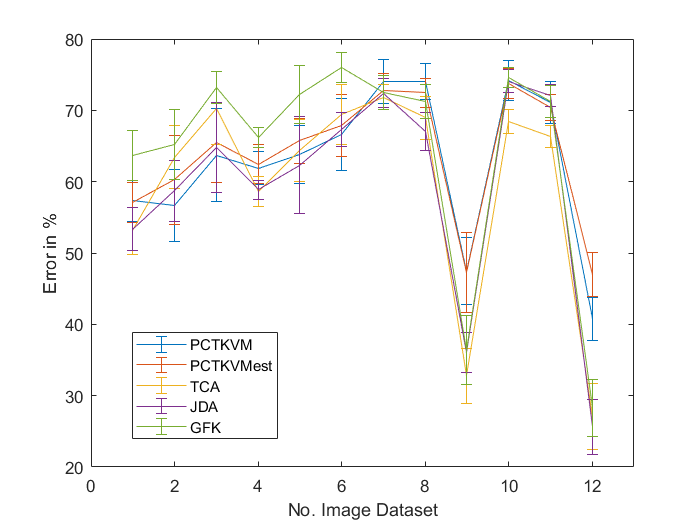
\includegraphics[width=1\linewidth]{figures/FiveTwoImageTL.png}
		\caption{\label{FigErrorImgTL}}
	\end{subfigure}%
	\begin{subfigure}{.5\textwidth}
		\centering
		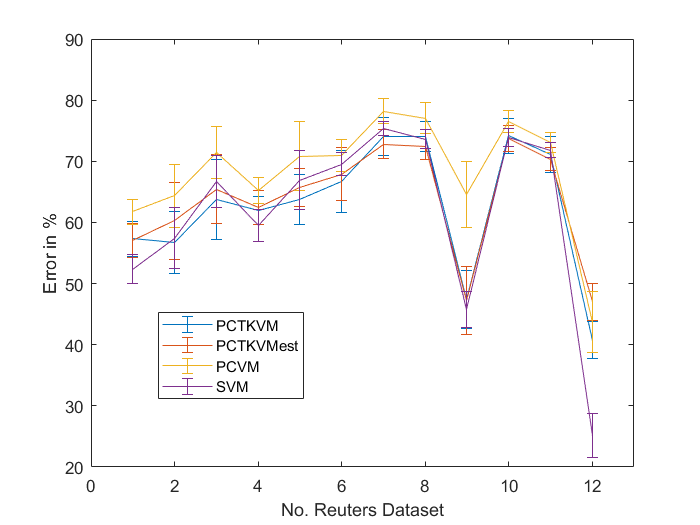
\includegraphics[width=1\linewidth]{figures/PerformanceImage.png}
		\caption{\label{FigErrorImgO}}
	\end{subfigure}
	\caption[Plot of mean Error and a standard Deviation on Image Dataset]{The plot of mean errors with standard deviation of the cross-validation. The left shows the transfer \acs{PCVM} in comparison with the other transfer learning solutions. The right side shows all \acs{PCVM}'s in comparison with \acs{SVM} and \acs{TKL}. A graph shows the error and a vertical bar shows the standard deviation. \label{FigErrorImgDatasetsB}}
\end{figure}

\begin{figure}[!]
	\centering
	\begin{subfigure}{.5\textwidth}
		\centering
		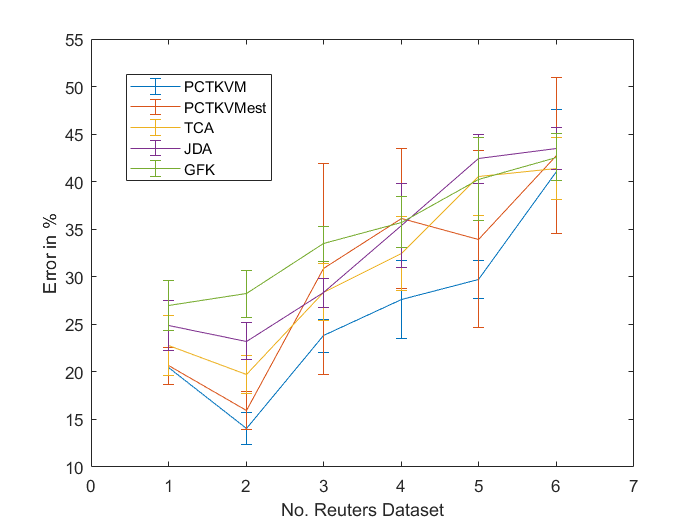
\includegraphics[width=1\linewidth]{figures/FiveTwoReutersTL.png}
		\caption{\label{FigErrorReuTL}}
	\end{subfigure}%
	\begin{subfigure}{.5\textwidth}
		\centering
		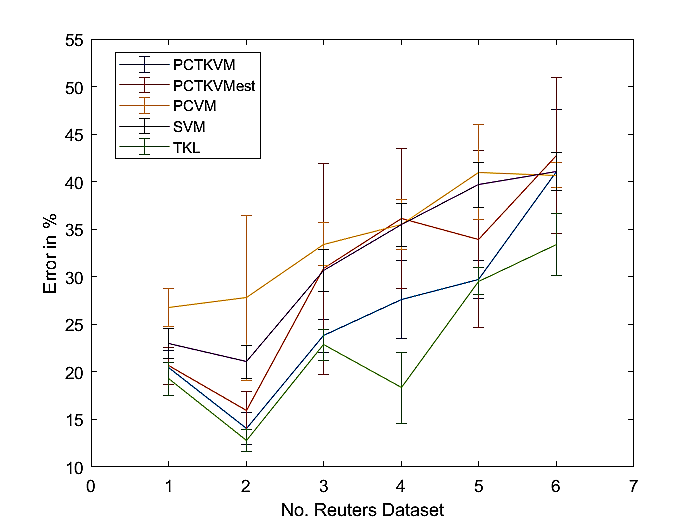
\includegraphics[width=1\linewidth]{figures/PerformanceReuters.png}
		\caption{\label{FigErrorReuO}}
	\end{subfigure}
	\caption[Plot of mean Error and standard Deviation on Reuters Dataset]{The plot of mean errors with standard deviation of the cross-validation. The left shows the transfer \acs{PCVM} in comparison with the other transfer learning solutions. The right side shows all \acs{PCVM}'s in comparison with \acs{SVM} and \acs{TKL}. A graph shows the error and a vertical bar shows the standard deviation. \label{FigErrorReutersDatasetsB}}
\end{figure}

\begin{table}[]
	\centering
	\resizebox{\textwidth}{!}{%
		\begin{tabular}{@{}ccccccccc@{}}
			\toprule
			\textbf{AUC Image}   & SVM   & PCVM  &  PCTKVM\textsubscript{$\theta$Est} & PCTKVM        & TCA   & JDA    & TKL            \\ \midrule
			C vs A               & 79.62 & 81.10 & 78.34 & 79.18          & 65.65 & 79.98 & 74.55 \\
			C vs D               & 64.36 & 89.85 & 95.12 & 96.98 & 58.86 & 72.98 		  & 68.76          \\
			C vs W               & 78.21 & 73.85 & 89.95 & 85.59          & 71.47 & 84.85 & 83.41 \\
			A vs C               & 74.93 & 73.48 & 74.31 & 72.29          & 66.36 & 71.37 & 69.78 \\
			A vs D               & 70.03 & 76.08 & 75.77 & 88.04 & 58.23 & 65.28 	      & 81.72          \\
			A vs W               & 77.70 & 73.40 & 81.35 & 82.82          & 66.82 & 72.82 & 80.80 \\
			D vs C               & 68.13 & 49.74 & 57.9 & 56.38          & 71.43 & 74.28 & 67.84 \\
			D vs A               & 76.25 & 35.30 & 45.64 & 45.02          & 79.09 & 78.97 & 77.51 \\
			D vs W               & 94.87 & 48.71 & 74.78 & 71.91          & 89.79 & 96.73 & 95.01 \\
			W vs C               & 58.39 & 56.29 & 56.08 & 57.20          & 62.92 & 70.04 & 63.22 \\
			W vs A               & 73.54 & 43.79 & 61.4 & 62.70          & 73.25 & 76.16 & 70.78 \\
			W vs D               & 72.48 & 89.56 & 93.61 & 97.21          & 73.36 & 79.56 & 92.26\\\midrule
			\textbf{AUC Reuters} & SVM   & PCVM  & PCTKVM\textsubscript{$\theta$Est} & PCTKVM      & TCA   & JDA   & TKL            \\\midrule
			Orgs vs People       & 81.14 & 80.29 & 88 & 88.62          & 83.45 & 80.34 & 90.43 \\
			People vs Orgs       & 82.23 & 81.08 & 91.48 & 92.64          & 85.98 & 82.39 & 93.61 \\
			Orgs vs Places       & 73.99 & 73.51 & 74.95 & 82.56          & 76.31 & 75.47 & 84.00 \\
			Places vs Orgs       & 69.50 & 69.97 & 77.35 & 80.21          & 72.86 & 68.59 & 89.50 \\
			Places vs People     & 59.36 & 63.11 & 71.77 & 77.15          & 60.95 & 58.72 & 76.57 \\
			People vs Places     & 47.77 & 57.78 & 55.25 & 54.97          & 54.35 & 49.15 & 66.63 \\ \bottomrule
	\end{tabular}}
	\caption[Complete Cross-Validtion Result of AUC]{Cross-validation comparison of the tested algorithms on 18 domain adaptation datasets by the AUC value. It shows the mean of the ten runs of cross-validation per dataset. The positive class is one, and the negative class is the composition of remaining classes.\label{BTableFTAUC}}
\end{table}


\begin{table}[]
	\centering
	\resizebox{\textwidth}{!}{%
		\begin{tabular}{@{}ccccccccc@{}}
			\toprule
			\textbf{N. SV. Image} & SVM    & PCVM   & PCTKVM\textsubscript{$\theta$Est} & PCTKVM & TCA    & JDA     & TKL    \\ \midrule
			C vs A                           & 556.70 & 125.80 & 87.6                               & 95.60  & 459.70 & 516.10 & 503.90 \\
			C vs D                           & 557.60 & 124.60 & 78.3                               & 87.80  & 466.80 & 522.20 & 522.30 \\
			C vs W                           & 557.30 & 126.40 & 82.2                               & 93.40  & 468.80 & 520.30 & 526.70 \\
			A vs C                           & 458.00 & 93.70  & 75.9                               & 79.20  & 356.30 & 416.70 & 412.30 \\
			A vs D                           & 455.80 & 92.70  & 62.4                               & 73.40  & 357.60 & 416.90 & 432.80 \\
			A vs W                           & 457.70 & 93.50  & 66.9                               & 76.70  & 357.00 & 416.10 & 429.30 \\
			D vs C                           & 78.50  & 20.50  & 18.7                               & 19.30  & 69.40  & 75.90  & 71.20  \\
			D vs A                           & 78.50  & 21.20  & 18.6                               & 18.90  & 69.30  & 76.00  & 72.60  \\
			D vs W                           & 78.50  & 20.80  & 19.2                               & 19.60  & 71.50  & 77.00  & 71.40  \\
			W vs C                           & 146.00 & 33.60  & 29.9                               & 31.70  & 119.70 & 137.00 & 127.90 \\
			W vs A                           & 146.70 & 33.90  & 29.5                               & 30.80  & 121.20 & 137.50 & 130.90 \\
			W vs D                           & 146.90 & 34.10  & 31                               & 32.10  & 122.30 & 137.50 & 126.70 \\ \midrule
			\textbf{N. SV. Reuters}        & SVM    & PCVM   & PCTKVM\textsubscript{$\theta$Est} & PCTKVM & TCA    & JDA    & TKL    \\ \midrule
			Orgs vs People                   & 514.60 & 33.80  & 2.7                               & 2.80   & 163.90 & 207.10 & 327.30 \\
			People vs Orgs                   & 526.20 & 54.10  & 2.6                               & 3.00   & 197.50 & 240.20 & 389.00 \\
			Orgs vs Places                   & 427.20 & 25.30  & 5.3                               & 3.10   & 155.50 & 187.20 & 355.00 \\
			Places vs Orgs                   & 464.00 & 30.10  & 2.2                               & 2.80   & 189.10 & 212.90 & 428.80 \\
			Places vs People                 & 477.70 & 58.30  & 2.9                               & 3.40   & 219.20 & 261.20 & 350.50 \\
			People vs Places                 & 484.40 & 80.00  & 2.4                               & 3.00   & 171.00 & 213.10 & 444.60 \\ \bottomrule
	\end{tabular}}
	\caption[Number of used support vectors from cross-validation]{A complete comparison of used support vectors in the cross-validation test over the 18 domain adaptation datasets. It shows the mean of the ten runs of cross-validation.\label{BTableFTNev}}
\end{table}
\begin{table}[]
	\centering
	\resizebox{\textwidth}{!}{%
		\begin{tabular}{@{}lllllllll@{}}
			\toprule
			\textbf{Time Image}   & SVM   & PCVM   & PCTKVM\textsubscript{$\theta$Est}& PCTKVM        & TCA   & JDA   & GFK   & TKL            \\ \midrule
			C vs A                & 0.11  & 468.91 & 33.19 & 35.10         & 1.95  & 1.37  & 0.71  & 0.78  \\
			C vs D                & 0.06  & 478.03 & 3.66 & 3.44 & 0.60  & 0.65  & 0.54  & 0.12           \\
			C vs W                & 0.07  & 490.87 & 6.03 & 6.87          & 0.74  & 0.74  & 0.56  & 0.16  \\
			A vs C                & 0.11  & 385.44 & 67.81 & 42.08         & 1.97  & 1.35  & 0.68  & 0.91  \\
			A vs D                & 0.04  & 385.38 & 4.59 & 4.37 & 0.41  & 0.51  & 0.46  & 0.07           \\
			A vs W                & 0.05  & 385.79 & 8.64 & 7.59          & 0.55  & 0.60  & 0.47  & 0.12  \\
			D vs C                & 0.04  & 68.15  & 25.94 & 26.44         & 0.55  & 0.61  & 0.40  & 0.71  \\
			D vs A                & 0.03  & 67.68  & 23.82 & 23.01         & 0.40  & 0.50  & 0.35  & 0.56  \\
			D vs W                & 0.01  & 69.87  & 5.14 & 5.54          & 0.06  & 0.13  & 0.21  & 0.07  \\
			W vs C                & 0.05  & 100.65 & 27.54 & 27.94         & 0.68  & 0.69  & 0.43  & 0.62  \\
			W vs A                & 0.04  & 102.59 & 29.39 & 26.62         & 0.51  & 0.58  & 0.38  & 0.43  \\
			W vs D                & 0.01  & 101.94 & 3.66 & 3.27          & 0.05  & 0.13  & 0.22  & 0.03  \\\midrule
			\textbf{Time Reuters} & SVM   & PCVM   & PCTKVM\textsubscript{$\theta$Est}& PCTKVM      & TCA   & JDA   & GFK   & TKL            \\\midrule
			Orgs vs People        & 15.59 & 694.52 & 15.32 & 20.35         & 20.95 & 24.13 & 44.65 & 15.82 \\
			People vs Orgs        & 14.66 & 656.70 & 15.61 & 20.29         & 21.08 & 24.72 & 43.79 & 15.69 \\
			Orgs vs Places        & 9.93  & 451.34 & 11.03 & 13.37         & 14.10 & 16.00 & 34.36 & 10.71 \\
			Places vs Orgs        & 10.20 & 474.43 & 11.3 & 14.87         & 13.72 & 15.72 & 35.77 & 10.88 \\
			Places vs People      & 11.55 & 525.75 & 11.92 & 15.46         & 15.23 & 17.39 & 39.16 & 11.98 \\
			People vs Places      & 9.27  & 459.54 & 11.48 & 12.83         & 12.31 & 14.82 & 22.30 & 9.67  \\ \bottomrule
	\end{tabular}}
	\caption[Time comparison from cross-validation]{Comparison of the absolute running time in seconds in the cross-validation test over the 18 datasets. It shows the mean time of the ten runs of cross-validation\label{BTableFTTime}}
\end{table}
\section{Complete Dataset Comparison}\label{BSecCom}
This section shows the results of the classifiers trained on the whole dataset. 
In general, the tables are showing the mean over five runs and are separated in the Reuters and image dataset.
In table \ref{BTableCompleteErr} are the error and \acs{RMSE} values shown.
This results are also plotted in figure \ref{FigErrorImgDatasetsB} for images and plotted in figure \ref{FigErrorReutersDatasetsB} for Reuters.
The numbers of a dataset is the order of the sets, shown for example in \ref{BTableFTErr}.
The \acs{AUC} values are shown in table \ref{BTableCompletAUC}.
For a complete overview over the used support vectors, see table \ref{BTableCompleteNvec}.
Finally, the computation time in second as the mean over five runs is shown in \ref{BTableCompleteTime}. 
\begin{table}[h]
	\centering
	\resizebox{\textwidth}{!}{%
		\begin{tabular}{@{}ccccccccc@{}}
			\toprule
			\textbf{Error Image}   & SVM   & PCVM  & PCTKVM\textsubscript{$\theta$Est}& PCTKVM         & TCA   & JDA   & GFK   & TKL            \\ \midrule
			C vs A                 & 46.66 & 55.80(1.06) & 50.71 (2.18)  & 46.26  (1.75)        & 44.89 & 42.17 & 59.92 & 44.05 \\
			C vs D                 & 51.59 & 64.97 (2.25)& 50.83 (4.51)  & 50.83 (4.06)& 54.14 & 56.69 & 58.60 & 54.78          \\
			C vs W                 & 59.32 & 66.31 (2.73)& 55.05 (3.95)  & 51.93  (2.48)        & 54.58 & 51.19 & 64.41 & 49.15 \\
			A vs C                 & 56.10 & 62.85 (1.62)& 56.81 (0.21)  & 55.10  (0.69)        & 54.23 & 54.59 & 59.75 & 54.05 \\
			A vs D                 & 54.78 & 68.15 (4.18)& 60    (2.6)  & 52.61 (3.17)& 62.42 & 65.61 & 61.78 & 52.87          \\
			A vs W                 & 61.69 & 71.12 (2.01)& 64.2  (3.22)  & 58.51  (1.55)        & 60.68 & 55.93 & 62.03 & 57.29 \\
			D vs C                 & 70.44 & 73.00 (1.3)&  67.14 (0.41) & 66.45  (1.11)        & 63.05 & 65.63 & 71.42 & 61.00 \\
			D vs A                 & 69.83 & 72.11 (1.63)& 66.12 (0.75)  & 63.82  (1.30)        & 61.59 & 62.63 & 66.39 & 60.96 \\
			D vs W                 & 37.63 & 60.20 (4.96)& 29.83 (3.12)  & 29.08   (3.99)       & 14.58 & 15.59 & 17.29 & 13.90 \\
			W vs C                 & 74.35 & 72.45 (0.84)& 67.16 (0.7)  & 67.03   (1.09)       & 67.94 & 68.12 & 71.15 & 65.00 \\
			W vs A                 & 67.85 & 71.84 (1.4)& 64.86  (1.87)& 64.61   (1.84)       & 64.41 & 66.81 & 66.91 & 62.00 \\
			W vs D                 & 15.29 & 37.71 (3.03)& 33.12 (1.49)  & 26.75   (1.01)       & 15.92 & 11.46 & 11.46 & 15.29 \\\midrule
			RSME                   & 55.46 & 64.71 (10.1) & 55.80(12.28)     & 52.75 (13.4)         & 51.53 & 51.37 & 55.93 & 49.19 \\\midrule
			\textbf{Error Reuters} & SVM   & PCVM  & PCTKVM\textsubscript{$\theta$Est}& PCTKVM       & TCA   & JDA   & GFK   & TKL            \\\midrule
			Orgs vs People         & 23.26 & 30.17(6)   &  19.97 (1.42)	    & 19.72  (0.86)        & 22.93 & 24.83 & 25.33 & 18.05 \\
			People vs Orgs         & 21.75 & 25.16(2.83) & 19.97 (1.42)	    & 13.76 (0.38)         & 20.45 & 24.17 & 27.49 & 12.29 \\
			Orgs vs Places         & 30.01 & 36.82 (5.24)& 33.27 (15.92)    & 24.20  (0.62)        & 28.19 & 27.04 & 32.69 & 23.20 \\
			Places vs Orgs         & 37.01 & 37.48 (2.34)& 33.27 (15.92)    & 33.94  (9.65)        & 30.31 & 34.65 & 37.70 & 16.73 \\
			Places vs People       & 39.28 & 41.30 (1.97)& 43.03 (14.37)    & 29.38   (0.33)       & 41.04 & 43.73 & 42.62 & 29.71 \\
			People vs Places       & 41.60 & 41.54 (0.90)& 43.03 (14.37)    & 39.74    (0)      & 47.08 & 44.57 & 43.64 & 33.05 \\\midrule
			RSME                   & 32.15 & 35.41(6.5) & 34.09 (8.0)    & 26.79 (9.67)         & 31.67 & 33.16 & 34.91 & 22.17 \\ \bottomrule
	\end{tabular}}
	\caption[Complete Dataset Result of Error]{The test result of the classifiers by using the whole 18 datasets. It shows the mean error over five runs.\label{BTableCompleteErr}}
\end{table}

\begin{figure}[!]
	\centering
	\begin{subfigure}{.5\textwidth}
		\centering
		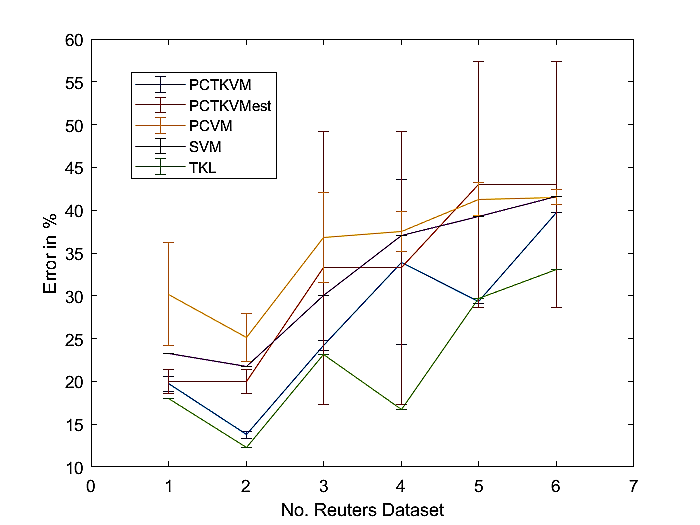
\includegraphics[width=1\linewidth]{figures/AverageReuters.png}
		\caption{\label{FigErrorAvReuTL}}
	\end{subfigure}%
	\begin{subfigure}{.5\textwidth}
		\centering
		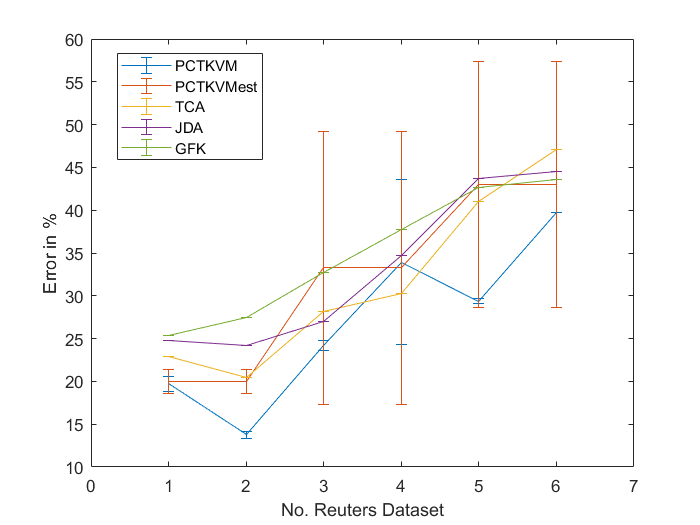
\includegraphics[width=1\linewidth]{figures/AverageReutersTL.png}
		\caption{\label{FigErrorAvReuO}}
	\end{subfigure}
	\begin{subfigure}{.5\textwidth}
		\centering
		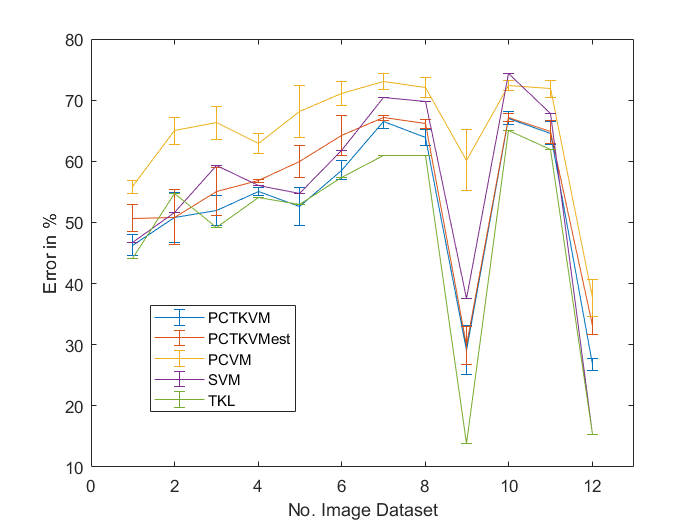
\includegraphics[width=1\linewidth]{figures/AverageImage.png}
		\caption{\label{FigErrorAvImTL}}
	\end{subfigure}%
	\begin{subfigure}{.5\textwidth}
		\centering
		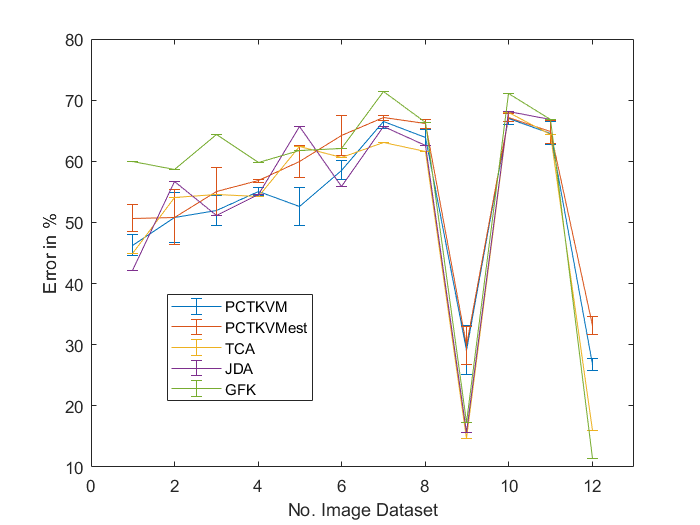
\includegraphics[width=1\linewidth]{figures/AverageImageTL.png}
		\caption{\label{FigErrorAvImO}}
	\end{subfigure}
	\caption[Plot of mean Error and standard Deviation on the whole Datasets]{The plot of mean errors with a standard deviation on the whole datasets. The left side shows all \acs{PCVM}'s in comparison with \acs{SVM} and \acs{TKL}. The right side shows all \acs{PCVM}'s in comparison to the other transfer learning solutions. The first row shows the result on Reuters and the second row illustrates the result on image dataset. A graph shows the error and a vertical bar shows the standard deviation. \label{FigErrorAv}}
\end{figure}


\begin{table}[]
	\centering
	\resizebox{\textwidth}{!}{%
		\begin{tabular}{@{}ccccccccc@{}}
			\toprule
			\textbf{AUC Image}   & SVM   & PCVM  & PCTKVM\textsubscript{$\theta$Est} & PCTKVM      & TCA   & JDA   & TKL            \\ \midrule
			C vs A               & 71.75 & 85.73 & 84.53     & 85.81          & 64.21 & 71.67 & 65.76 \\
			C vs D               & 56.78 & 94.85 & 93.37     & 90.78 & 60.40 & 68.45 		  & 51.49          \\
			C vs W               & 67.15 & 85.61 & 90.15     & 95.74          & 50.75 & 64.92 & 78.47 \\
			A vs C               & 74.87 & 73.38 & 78.09     & 76.09          & 58.27 & 73.57 & 74.39 \\
			A vs D               & 72.93 & 78.89 & 97.26     & 88.37 & 57.53 & 71.84 		  & 78.68          \\
			A vs W               & 86.48 & 68.09 & 86.57     & 80.38          & 77.50 & 75.36 & 82.81 \\
			D vs C               & 76.33 & 52.52 & 61.55     & 50.66          & 82.63 & 80.23 & 78.78 \\
			D vs A               & 79.78 & 54.52 & 66.8    & 52.47          & 85.83 & 86.81 & 82.57 \\
			D vs W               & 96.36 & 52.31 & 73.54     & 70.18          & 76.33 & 98.03 & 97.24 \\
			W vs C               & 66.91 & 54.76 & 69.74     & 66.82          & 70.11 & 77.41 & 71.79 \\
			W vs A               & 72.46 & 49.93 & 62.46     & 64.64          & 74.36 & 84.21 & 77.75 \\
			W vs D               & 80.69 & 84.91 & 93.05     & 98.70          & 84.02 & 90.29 & 93.28 \\\midrule
			\textbf{AUC Reuters} & SVM   & PCVM  & PCTKVM\textsubscript{$\theta$Est} & PCTKVM      & TCA   & JDA    & TKL            \\\midrule
			Orgs vs People       & 79.97 & 79.00 & 89     & 89.54          & 83.80 & 81.13  & 90.70 \\
			People vs Orgs       & 80.35 & 81.60 & 89     & 92.57          & 84.27 & 81.95  & 93.69 \\
			Orgs vs Places       & 72.83 & 70.96 & 74.47     & 83.55          & 77.08 & 76.46  & 84.79 \\
			Places vs Orgs       & 66.40 & 69.89 & 74.47     & 87.33          & 74.64 & 69.55  & 91.34 \\
			Places vs People     & 56.36 & 60.64 & 66.2     & 77.03          & 56.78 & 56.43  & 76.31 \\
			People vs Places     & 42.59 & 51.82 & 66.2     & 58.40          & 39.85 & 45.87  & 66.95 \\ \bottomrule
	\end{tabular}}
	\caption[Complete Dataset Result of AUC]{The test result of the classifiers by using the whole 18 datasets. It shows the mean AUC value over five runs. The positive class is one, and the negative class is the composition of remaining classes.\label{BTableCompletAUC}}
\end{table}

\begin{table}[]
	\centering
	\resizebox{\textwidth}{!}{%
		\begin{tabular}{@{}ccccccccc@{}}
			\toprule
			\textbf{N. SV. Image} & SVM     & PCVM   & PCTKVM\textsubscript{$\theta$Est} & PCTKVM & TCA    & JDA   & TKL    \\ \midrule
			C vs A                           & 1098.00 & 242.80 & 109.8                                   & 153.00 & 818.00 & 973.00 & 937.00 \\
			C vs D                           & 1098.00 & 257.20 & 105.8                                   & 130.60 & 828.00 & 976.00 & 983.00 \\
			C vs W                           & 1098.00 & 246.20 & 116.2                                   & 137.00 & 834.00 & 980.00 & 976.50 \\
			A vs C                           & 898.00  & 187.40 & 113                                   & 128.80 & 577.00 & 726.00 & 749.00 \\
			A vs D                           & 898.00  & 184.00 & 93                                   & 114.60 & 581.00 & 729.00 & 829.00 \\
			A vs W                           & 898.00  & 188.40 & 101.6                                   & 112.60 & 588.00 & 742.00 & 791.00 \\
			D vs C                           & 157.00  & 39.80  & 35.6                                   & 37.60  & 130.00 & 149.00 & 137.00 \\
			D vs A                           & 157.00  & 37.20  & 32.8                                   & 35.00  & 134.00 & 149.00 & 139.00 \\
			D vs W                           & 157.00  & 41.40  & 33                                   & 36.00  & 138.00 & 149.00 & 130.00 \\
			W vs C                           & 295.00  & 65.20  & 55                                   & 53.80  & 214.00 & 273.00 & 248.00 \\
			W vs A                           & 295.00  & 64.00  & 51.4                                   & 53.80  & 210.00 & 270.00 & 248.00 \\
			W vs D                           & 295.00  & 63.40  & 53.4                                   & 55.20  & 224.00 & 275.00 & 239.00 \\ \midrule
			\textbf{N. SV. Reuters}        & SVM     & PCVM   & PCTKVM\textsubscript{$\theta$Est} & PCTKVM & TCA    & JDA   & TKL    \\ \midrule
			Orgs vs People                   & 850.00  & 66.60  & 3                                  & 2.40   & 280.00 & 329.00 & 604.00 \\
			People vs Orgs                   & 867.50  & 53.60  & 3                                  & 2.80   & 309.00 & 356.50 & 667.00 \\
			Orgs vs Places                   & 708.00  & 60.80  & 2                                  & 2.80   & 265.00 & 274.00 & 679.00 \\
			Places vs Orgs                   & 752.00  & 43.00  & 2                                  & 3.00   & 291.50 & 297.00 & 746.50 \\
			Places vs People                 & 845.00  & 48.00  & 4                                  & 4.00   & 362.00 & 447.00 & 659.00 \\
			People vs Places                 & 838.50  & 54.00  & 4                                  & 2.20   & 315.50 & 390.50 & 748.50 \\ \bottomrule
	\end{tabular}}
	\caption[Complete number of used support vectors]{Comparison of the number of used support vectors for the whole 18 datasets. It shows the mean number over five runs.\label{BTableCompleteNvec}}
\end{table}

\begin{table}[]
	\centering
	\resizebox{\textwidth}{!}{%
		\begin{tabular}{@{}ccccccccc@{}}
			\toprule
			\textbf{Time Image}   & SVM   & PCVM    &PCTKVM\textsubscript{$\theta$Est}& PCTKVM      & TCA   & JDA    & GFK   & TKL            \\ \midrule
			C vs A                & 0.41  & 1561.72 & 124.38     & 95.19          & 12.72 & 5.66   & 1.58  & 1.70  \\
			C vs D                & 0.19  & 1534.87 & 13.51     & 10.20 & 3.85  & 2.21   & 1.04  & 0.28           \\
			C vs W                & 0.22  & 1523.58 & 17.97     & 39.27          & 4.58  & 2.61   & 1.10  & 0.71  \\
			A vs C                & 0.36  & 1167.97 & 133.97     & 77.53          & 12.07 & 5.51   & 1.53  & 2.01  \\
			A vs D                & 0.14  & 1188.29 & 11.61     & 9.76  & 2.55  & 1.76   & 0.97  & 0.22           \\
			A vs W                & 0.16  & 1175.60 & 17.16     & 63.73          & 3.27  & 2.09   & 1.00  & 0.61  \\
			D vs C                & 0.12  & 104.43  & 80.73     & 70.93          & 3.31  & 2.09   & 0.81  & 1.43  \\
			D vs A                & 0.10  & 106.09  & 72.52     & 50.58          & 2.27  & 1.68   & 0.72  & 1.04  \\
			D vs W                & 0.02  & 106.48  & 14.7     & 14.68          & 0.24  & 0.36   & 0.29  & 0.43  \\
			W vs C                & 0.15  & 179.01  & 81.85     & 92.44          & 4.30  & 2.62   & 0.93  & 1.65  \\
			W vs A                & 0.12  & 177.99  & 66.65     & 62.21          & 3.12  & 2.03   & 0.78  & 1.12  \\
			W vs D                & 0.02  & 177.49  & 10.66     & 8.14           & 0.26  & 0.37   & 0.32  & 0.11  \\\midrule
			\textbf{Time Reuters} & SVM   & PCVM    & PCTKVM\textsubscript{$\theta$Est} & PCTKVM        & TCA   & JDA    & GFK   & TKL            \\\midrule
			Orgs vs People        & 49.48 & 2256.50 & 64.23    & 61.25          & 73.74 & 103.73 & 33.24 & 49.19 \\
			People vs Orgs        & 47.16 & 2024.11 & 64.23    & 67.62          & 69.82 & 100.04 & 32.68 & 47.86 \\
			Orgs vs Places        & 34.79 & 1529.51 & 45.37    & 47.62          & 51.44 & 69.37  & 27.66 & 34.53 \\
			Places vs Orgs        & 33.18 & 1488.56 & 45.37    & 52.41          & 46.38 & 66.13  & 27.28 & 36.25 \\
			Places vs People      & 38.01 & 1794.56 & 51.49    & 56.30          & 63.67 & 88.54  & 30.87 & 43.54 \\
			People vs Places      & 37.11 & 1641.59 & 51.49    & 60.23          & 53.68 & 77.32  & 28.37 & 38.70 \\ \bottomrule
	\end{tabular}}
	\caption[Time comparison of whole dataset]{Comparison of the absolute running time in second for the whole 18 datasets as mean. It shows the mean time of five runs.\label{BTableCompleteTime}}
\end{table}

\chapter{Details of Algorithms}\label{appac}
In this appendix, the detailed steps for the \acs{PCTKVM} algorithm are presented.
We omit it the steps, which are already described in \acs{PCVM} and \acs{TKL} for clarity.
The complete algorithm procedure is shown in algorithm \ref{PCTKVMComplete}.\\
We also have extended the algorithm with the faster approach, where the dissimilar matrix is reused over tasks.
Furthermore, we have extended the pseudo code with the option, which allows the user to decide, whether he wants to specify the $\theta$ or proceed with the estimation.
If one decides to choose a $\theta$ on his own, then the model has two parameters: The width of the Gaussian kernel and the $\zeta$ eigenspectrum dumping factor.
Moreover, \acs{PCTKVM} algorithm has following algorithm parameter:
The \acs{PCTKVM} supports the standard Gaussian kernel, the new Gaussian kernel from \eqref{EqRBFAKernel} and the Laplacian kernel.
However, we strongly recommend the use of the new Gaussian kernel.\\
Furthermore the number of iterations \textit{niter} for the \acs{PCVM} can be specified and the convergence criteria as a \textit{threshold}.
In algorithm \ref{PseudoCodePcvm} the pseudo code for the \acs{PCVM} and a line explanation can be found.

\begin{algorithm}[!]
	\caption{Probabilistic Classification Transfer Kernel Vector Machine }\label{PCTKVMComplete}
	\begin{algorithmic}[1]
		\Require Input Data $\mathbf{K} = [\mathbf{Z};\mathbf{X}]$ as $N_\mathcal{Z}$ sized training and $N_\mathcal{X}$ sized text set; $\mathbf{Y}$ as $N$ sized training label vector; kernel(-type) \textit{ker}; eigenspectrum dumping factor $\zeta$; $\theta$ as kernel parameter; \textit{niter} as maximal number of iterations; \textit{threshold} $\tau$ as convergence criteria; \textbf{InitVector} as $N_\mathcal{Z}$-sized initialization vector.
		\Ensure Weight vector $\mathbf{w}$; bias $b$, kernel parameter $\theta$; transfer kernel $\expP{\mathbf{K}}_\mathcal{A}$.
		\State $\mathbf{D}$ = calculate\_Dissimilarity\_Matrix($\mathbf{K}$);
		\If{$\theta == -1$}
		\State $\theta$ = theta\_Estimation($\mathbf{D}$);  \Comment{According to section \eqref{InSubSecTheta}}
		\EndIf
		\State [$\mathbf{K}_\mathcal{Z}$, $\mathbf{K}_\mathcal{X}$,$\mathbf{K}_\mathcal{ZX}$]=compute\_Gaussian\_Kernel($\mathbf{D}$,\textit{ker},$\theta$),
		\State [$\{\mathbf{\Lambda}_\mathcal{X}, \mathbf{U}_\mathcal{X}\}$]= eigenDecompose($\mathbf{K}_\mathcal{X}$)  \Comment{Eq. \eqref{EqEigsProb}}
		\State [$\expP{\mathbf{U}}_\mathcal{Z}$] =extrapolate\_Eigensystem($\mathbf{K}_\mathcal{ZX},\mathbf{U}_\mathcal{X},\boldsymbol{\Lambda}_\mathcal{X}^{-1}$) \Comment{Eq. \eqref{EqExtraEigs}}
		\State [$\boldsymbol{\Lambda}$]=quadratic\_Programming($\mathbf{Q},\mathbf{C},r$)  \Comment{Eq. \eqref{EqTklQP} and constrains \eqref{EqTklQPCons}}
		\State		[$\expP{\mathbf{K}}_\mathcal{A}$]=compute\_Extrapolated\_Kernel($\expP{\mathbf{U}}_\mathcal{Z},\boldsymbol{\Lambda},\mathbf{U}_\mathcal{X}$) \Comment{Eq. \eqref{EqTKLKernel}}
		\State	[$\mathbf{w},b$] = initialize(\textbf{initVector});
		\State \textbf{nonZero} = determine\_nonZero\_Vector($\mathbf{w}$); 
		\For{$i=1$ to \textit{niter}}
		\State $\mathbf{w}^{new}$ = weight\_Update($\expP{\mathbf{K}}_{\mathcal{Z}},\mathbf{w,Y,nonZero}$);   \Comment{Eq. \eqref{EqPcvmUpdateW}}
		\State $b^{new}$ = bias\_update($\expP{\mathbf{K}}_{\mathcal{Z}},b\mathbf{,Y,nonZero}$); \Comment{Eq. \eqref{EqPcvmUpdateb}}
		\State $\theta^{new}$ = parameter\_update($\expP{\mathbf{K}}_{\mathcal{Z}},\mathbf{Y},\mathit{ker},\theta,\mathbf{w}^{new},b^{new},\mathbf{nonZero}$); \Comment{Eq. \eqref{EqPcvmDevTheta}}
		\State $\mathbf{nonZero}^{new}$ = determine\_nonZero\_Vector($\mathbf{w}^{new}$);
		\If{max(abs($\mathbf{w}^{new}-\mathbf{w}$)) $<$ $\tau$}
		\State break;
		\Else
		\State continue;
		\EndIf
		\EndFor
	\end{algorithmic}
\end{algorithm}

\begin{algorithm}[H]
	\caption{Probabilistic Classification Vector Machine}\label{PseudoCodePcvm}	
	\begin{algorithmic}[1]
		\Require $\mathbf{I}$ =\{\textbf{X,Y}\} = $\{(x_n,y_n)\}_{n=1}^{N}$ as $N_\mathcal{Z}$ sized training set;
		\textit{ker} as kernel type; The kernel parameter $\theta$; \textit{niter} as maximal number of iterations; \textit{threshold} $\tau$ as convergence criteria; \textbf{InitVector} as $N_\mathcal{Z}$-sized initialization vector.
		\Ensure Weight Vector $\mathbf{w}$, bias $b$ and the kernel parameter $\theta$.
		\State	[$\mathbf{w},b$] = initialize(\textbf{initVector});
		\State \textbf{nonZero} = determine\_nonZero\_Vector($\mathbf{w}$); 
		\For{$i=1$ to \textit{niter}}
		\State $\Phi$ = Calculate\_Kernel($\mathbf{X,Y}$,\textit{ker},$\theta$); 
		\State $\mathbf{w}^{new}$ = weight\_update($\mathbf{\Phi,w,Y,nonZero}$);  
		\State $b^{new}$ = bias\_update($\mathbf{\Phi},b,\mathbf{Y,nonZero}$);
		\State $\theta^{new}$ = parameter\_update($\mathbf{\Phi,X,Y},\mathit{ker},\theta,\mathbf{w}^{new},b^{new},\mathbf{nonZero}$);
		\State $\mathbf{nonZero}^{new}$ = determine\_nonZero\_Vector($\mathbf{w}^{new}$);
		\If{max(abs($\mathbf{w}^{new}-\mathbf{w}$)) $<$ $\tau$ }
		\State break;
		\Else
		\State continue;
		\EndIf
		\EndFor
	\end{algorithmic}
\end{algorithm}
\algcomment{Explanation of the Steps within the Algorithm.
	\begin{enumerate}[noitemsep]
		\item Line 1 and 2: (Random) initialization of the weight vector $\mathbf{w}$ with $N$-sized \textbf{initVector} and bias $b$. Determining non-zero elements in $\mathbf{w}$ and save it as an index to \textbf{nonZero}.
		\item Line 4: Calculate the kernel $\Phi$.
		\item Line 5 and 6: Update $\mathbf{w}$ and $b$ with \eqref{EqPcvmUpdateW} and \eqref{EqPcvmUpdateb} respectively.
		\item Line 7: Solve optimization problem based on \eqref{EqPcvmDevTheta}.
		\item Line 9-15: Determine the convergence by comparing the difference of $\mathbf{w}^{new}$ and $\mathbf{w}$ against the threshold. Break if convergence happens, otherwise continue.
\end{enumerate}}\\


%% Bibliography
\bibliography{main}
\bibliographystyle{plaindin}




\end{document}

%TODO: Mehr allgemeine Einführung
%TODO: Ausformulieren
%TODO: RT Transfer- erst eine allgemeinere Intro - Themensetzung - dann erst
%
%
%- 'The MMD is calculated by samples ... ' - Abschnitt checken warum RKHS notwendig
%
%
%- 'With this, the kernel can be rewritten' - ich denke es ist nicht klar warum das hier sonst nicht geht
%
%- 'domain data where z i ? X_Z as single observation' - ich glaube die Notation ist nicht ganz klar
%
%------------ Notation--------------
%- Domain D, X, Z - pruefen (auch mal \cal mal ohne)
%- two labels, e. g. Y = -1, +1 --> (\{, \})
%- 'N' - als Anzahl Klassen ist eher unueblich - wird weiter hinten auch als Anzahl sample (normal) verwendet
%- ich finde die Notation in 1.3. etwas unnoetig kompliziert
